
\documentclass[a4paper,11pt]{scrreprt}

%%-------------- Grund Konfiguration (deutsch, 8bit) -----------------
\usepackage{lmodern}
%\usepackage{cm-super}
\usepackage[ngerman]{babel}% deutsche Trennmuster
\usepackage[T1]{fontenc}% --> usrguide und fntguide
\usepackage[utf8]{inputenc}

\usepackage{babelbib}

%----------------------code
\usepackage{listings}

\lstloadlanguages{Java,sh,bash,Haskell,HTML,PHP,XML}

\lstdefinelanguage{FSharp}
                {
                alsoletter={-,>},
                morekeywords={let, new, elif, match, with, rec, open, module, namespace, type, of, member, and, for, in, do, begin, end, fun, function, try, mutable, if, then, else, when, ,and,->},
    			keywordstyle=\color{blue},
    			sensitive=false,
    			morecomment=[l][\color{green}]{///},
    			morecomment=[l][\color{green}]{//},
    			morecomment=[s][\color{green}]{{(*}{*)}},
    			morestring=[b]",
    			stringstyle=\color{red}
    			}
\renewcommand{\lstlistingname}{Listing}
\renewcommand{\lstlistlistingname}{Listingverzeichnis}



\usepackage{faktor}

\usepackage{array}

\usepackage{graphicx}
\usepackage{caption}
\usepackage[table]{xcolor}
\usepackage{tikz}


\usepackage{fancyhdr}
\pagestyle{fancy}
\fancyhf{}
\lhead{\rightmark}
\rfoot{\thepage}
%\renewcommand{\footrulewidth}{0.4pt}
%\lhead{Kapitel \thechapter}
\usepackage{ifthen}
\usepackage{amssymb}
\usepackage{amsmath}
\usepackage{amsthm}
\usepackage{pifont}% http://ctan.org/pkg/pifont
\newcommand{\cmark}{\ding{51}}%
\newcommand{\xmark}{\ding{55}}%


\usepackage{framed}
\usepackage{url}


\newtheorem{lm}{Lemma}
\newtheorem{satz}{Satz}
\newtheorem{thrm}{Theorem}
\newtheorem*{cor}{Folgerung}
\newtheorem*{ern}{Erinnerung}
\theoremstyle{definition}

\newtheorem{defi}{Definition}

\colorlet{shadecolor}{blue!10}
\newenvironment{df}
  {\begin{shaded}\begin{defi}}
  {\end{defi}\end{shaded}}

\newenvironment{lsg}{
\begin{framed}\begin{ls}
}{
\end{ls}\end{framed}
}

\newtheorem*{pro}{Prolog}

\newtheorem*{lz}{Lernziele}

\newtheorem{rk}{Bemerkung}

\newtheorem*{ntt}{Notation}
\newenvironment{nt}
	{\begin{shaded}\begin{ntt}}
	{\end{ntt}\end{shaded}}

\newtheorem{bsp}{Beispiel}

\newtheorem*{alg}{Algorithmus}

\newtheorem{ueb}{\"Ubung}
\newtheorem*{ls}{Lösung}
\newtheorem*{wrn}{Warnung}
\newtheorem*{axi}{Axiom}


% Answer boxes
\newcommand{\answerspace}[2][n]{%
    \par\smallskip
    \begingroup
    \if#1r\hrule\fi
    \baselineskip=\dimexpr#2/100\relax
    \lineskip=0pt \parindent=0pt
    \count255=0
    \loop\ifnum\count255<100
    \advance\count255 by 1
    \leavevmode\vbox to\baselineskip{}
    \if#1r\vrule\hfill\vrule\fi\endgraf
    \repeat
    \if#1r\hrule\fi
    \smallskip
    \endgroup
}


\newcommand{\rs}{\upharpoonright}
\newcommand{\gwo}{\vartriangleleft}
\newcommand{\N}{\mathbb{N}}
\newcommand{\Z}{\mathbb{Z}}
\newcommand{\Q}{\mathbb{Q}}
\newcommand{\R}{\mathbb{R}}
\renewcommand{\P}{\mathbb{P}}
\newcommand{\modn}{\equiv_n}
\newcommand{\p}{\mathsf{P}}
\newcommand{\g}{\mathsf{G}}
\newcommand{\z}{\mathsf{z}}
\newcommand{\true}{\mathsf{true}}
\newcommand{\false}{\mathsf{false}}
\newcommand{\fnot}{\mathsf{not}}
\newcommand{\for}{\mathsf{or}}
\newcommand{\fand}{\mathsf{and}}

\renewcommand{\labelenumi}{\alph{enumi})}
\renewcommand{\labelitemi}{\textbf{-}}

\addto\captionsngerman{\renewcommand{\proofname}{\textsf{Beweis}}}




\begin{document}

\newboolean{ml} %musterloesung ja/nein
\setboolean{ml}{\solutionboolean}


\title{Grundlagen und Diskrete Mathematik}


\date{}
\maketitle

\tableofcontents

1.2\chapter{Grundbegriffe und elementare Logik}


Am Anfang aller Logik steht\dots
\begin{quote}
Wenn ``Doken'' stets ``derig'' sind und wenn es ``Raken'' gibt die auch ``Doken'' sind, dann gibt es
derige Raken und alle underigen Raken sind keine Doken.
\end{quote}
 \dots die Erkenntnis, dass
gewisse Argumente unabhängig von deren Inhalt aber aufgrund ihrer Struktur als eindeutig
schlüssig/korrekt identifizierbar sind. Dieses Kapitel gibt Ihnen eine informelle Einführung in die Prädikatenlogik.

\section*{Beispiele für Anwendungen in der Informatik}
\begin{itemize}
\item Grundlage für die Entwicklung einer soliden ``Theorie der Informatik''.
\item Künstliche Intelligenz, Wissensrepräsentation, Expertensysteme.
\item Allgegenwärtig in der Programmierung (z.B. ``if \dots then \dots else\dots''-Befehle).
\item Formale Verifikation der Korrektheit von Programmen.
\end{itemize}



\section*{Lernziele}
Sie kennen die Konzepte von
\begin{itemize}
\item Aussagen und Prädikaten.
\item universeller und existenzieller Quantifikation.
\end{itemize}
Sie verstehen wie
\begin{itemize}
\item durch Implikation, Äquivalenz, Negation, Konjunktion und Disjunktion neue Aussagen und Prädikate aus bereits bestehenden gewonnen werden.
\item durch Quantifikation von Prädikaten neue Aussagen und Prädikate gewonnen werden.
\end{itemize}
Sie sind in der Lage
\begin{itemize}
\item natürlichsprachliche (mathematische) Aussagen in der Sprache der Prädikatenlogik zu formalisieren.
\item mittels Fallunterscheidung, Widerspruchsargumenten und Kontraposition einfache mathematische Tatsachen zu beweisen.
\end{itemize}
Sie bewerten
\begin{itemize}
\item einfache Beweise und Argumente bezüglich ihrer Korrektheit und Stringenz.
\end{itemize}

\section*{Literatur und Links}
Ergänzende Literatur:
\begin{itemize}
\item  \cite{diskreteStrukturen} Kapitel 1.2 bis 1.4.
\item \cite{hartmann} Kapitel 2.
\item \cite{haggarty} Kapitel 2.
\end{itemize}
Weiterführende Literatur:
\begin{itemize}
\item \cite{flum} ganzes Buch.
\end{itemize}
Nützliche Links:
\begin{itemize}
\item \url{http://de.wikipedia.org/wiki/Pr%C3%A4dikatenlogik_erster_Stufe}
\item \url{https://openlogicproject.org/}
\end{itemize}

\section{Aussagen, Prädikate und Quantoren}

Wir werden im folgenden Abschnitt auf pragmatische Art und Weise die grundlegenden Konzepte der
Logik und Mathematik
kennenlernen. Um nicht nur langweilige Beispiele machen zu können, werden wir in diesem Kapitel auf
gewisse mathematische Begriffe wie z.b. ``natürliche Zahlen'' $(0,1,2,\dots)$ oder
``Primzahlen'' $(2,3,5,7,11\dots)$  zurückgreifen, ohne diese vorher sauber eingeführt zu haben. Die Anschauung,
welche Sie von der Schule mitbringen, sollte aber ausreichen um die Beispiele zu
verstehen.

\begin{df}
 Unter einer \textit{Aussage} wollen wir ein ``sprachliches Gebilde'' oder Ausdruck verstehen, welchem ein Wahrheitswert ``wahr'' oder ``falsch'' zugeordnet werden kann.
\end{df}

\begin{rk}
  Obwohl nach Definition jede Aussage einen eindeutigen Wahrheitswert besitzt, bedeutet dies nicht, dass dieser bekannt sein muss. Der Satz ``es gibt unendlich viele Primzahlen'' war beispielsweise bereits eine Aussage, bevor man wusste, dass er wahr ist.
\end{rk}

\begin{bsp}
 Einige Beispiele für Aussagen mit ihren Wahrheitswerten:
\begin{enumerate}
  \item ``$3+4=106$'' (falsch)
  \item ``Jede natürliche Zahl ist entweder durch $2$ oder durch $3$ teilbar.'' (falsch)
  \item ``Es gibt unendlich viele natürliche Zahlen.'' (wahr)
\end{enumerate}
\end{bsp}

\begin{rk}
Wir sagen, dass eine Variable $x$ frei in einem Ausdruck $A$ vorkommt, falls $x$ weder für einen noch für eine Menge von konkreten Werten steht, sondern einen reinen ``Platzhalter'' darstellt. Beispiele in denen die Variable $x$ frei vorkommt sind: ``$x<3$'' oder ``$x$ ist ein Tisch''. Im Gegensatz dazu kommt $x$ in ``alle $x$, die durch $4$ teilbar sind, sind gerade'' nicht frei vor, weil in dieser Aussage die Gesamtheit (Menge) aller möglichen Belegungen von $x$ betrachtet wird. In einem Ausdruck können beliebig viele Variablen frei vorkommen und wir schreiben $A(x,y,z,\dots)$, um anzuzeigen, dass in einem Ausdruck $A$ die Variablen $x,y,z,\dots$ frei vorkommen.
\end{rk}

\begin{df}
Es sei $n$ eine natürliche Zahl. Ein Ausdruck, in dem $n$ viele Variablen frei vorkommen und der bei Belegung aller freien Variablen in eine Aussage übergeht, nennen wir ein \textit{$n$-stelliges Prädikat}.
\end{df}

\begin{rk}
  Aussagen sind $0$-stellige Prädikate.
\end{rk}

\begin{rk}
  Ist $A(x)$ ein Prädikat und ist $y$ ein mathematisches Objekt (z.B. $y=17$) so, dass $A(y)$ eine wahre Aussage ist, dann sagen wir, dass das Prädikat (manchmal auch die Eigenschaft) $A$ auf $y$ zutrifft. Das Prädikat $x>100$ trifft zum Beispiel auf die Zahl $232$ zu, weil $232>100$ eine wahre Aussage ist.
\end{rk}

\begin{bsp}
  Einige Beispiele\footnote{Die Zeichenfolge ``$:=$'' steht für ``ist definiert als'' oder ``ist per Definition gleich''.} für Prädikate:
  \begin{enumerate}
  \item $P(p):= $\,``$p$ ist eine Primzahl.''
  \item $T(x):= $\,``$x$ ist eine durch $21$ teilbare ganze Zahl.''
  \item $G(r):= $\,``$r>0$''
  \item $Q(x,y):= $\,``$x^2+14x-15=y$''
  \end{enumerate}
  Die Aussagen
  \begin{align*}
  &T(42)& 	    &P(7)&		&Q(2,17)&\\
  &T(357)&  &P(2)& 	&Q(1,0)&
  \end{align*}
  sind alle wahr. Deshalb können wir, entsprechend der vorhergehenden Bemerkung, z.B. ``$T$ trifft auf $42$'' zu oder auch ``$7$ hat die Eigenschaft $P$'' sagen.
\end{bsp}

\begin{bsp}
  Weitere Beispiele für Prädikate:
  \begin{itemize}
    \item $A(x,y) := x + y < 10$ ist ein zweistelliges Pädikat mit den freien Variablen $x$ und $y$.
    \item $B(x,y,z) := x + y < z$ ist ein dreistelliges Prädikat.
    \item Wenn wir die Variable $z$ in $B$ mit dem Wert $10$ belegen, dann erhalten wir das zweistellige Prädikat $B(x,y,10)$, welches gleichbedeutend mit dem Prädikat $A$ ist.
  \end{itemize}
\end{bsp}

\subsection*{Junktoren}
Aus gegebenen Aussagen lassen sich durch Verknüpfung neue komplexere Aussagen
gewinnen. Betrachten wir zum Beispiel die Aussagen
\[
A:=\text{``}78\text{ ist keine Primzahl}
\]
und
\[
 B:=``15\text{ ist keine Primzahl}'',
\]
so können wir eine neue Aussage, nennen wir sie $C$, betrachten. $C$ soll ausdrücken, dass sowohl $A$ als auch $B$ wahr ist, d.h.
\[
 C:=\text{``}78\text{ ist keine Primzahl \textbf{und} }15\text{ ist keine Primzahl}\text{''}
\]
oder etwas anders formuliert (aber mit gleichem Wahrheitswert)
\[
 C:=\text{``weder die }15\text{ noch die }78\text{ ist eine Primzahl}\text{''}.
\]

Wir werden nun einige abkürzende Schreibweisen einführen um bequem über solche zusammengesetzten Aussagen sprechen zu können.

\begin{df}
Es seien $A$ und $B$ beliebige Prädikate. Wir führen folgende abkürzende Schreibweisen ein:
\begin{itemize}
\item $\neg A$ (gesprochen: Nicht $A$) ist das Prädikat, welches (für jede Belegung) genau dann wahr ist, wenn $A$ falsch ist.
 \item $A\wedge B$ (gesprochen: $A$ und $B$)  ist das Prädikat, welches (für jede Belegung) genau dann wahr ist, wenn sowohl $A$ als auch $B$ wahr sind.
\item $A\vee B$ (gesprochen: $A$ oder $B$)  ist das Prädikat, welches (für jede Belegung) genau dann wahr ist, wenn $A$ wahr ist oder $B$ wahr ist (oder beide wahr sind).
\item $A\Rightarrow B$ (gesprochen: $A$ impliziert $B$) ist das Prädikat, welches (für jede Belegung) genau dann wahr ist, wenn $\neg A\vee B$ wahr ist.
\item $A\Leftrightarrow B$ (gesprochen: $A$ äquivalent $B$)  ist das Prädikat, welches (für jede Belegung) genau dann wahr ist, wenn $A\Rightarrow B$ und $B\Rightarrow A$ wahr sind.
\end{itemize}
Die Zeichen $\neg,\Rightarrow,\wedge$ und $\vee$ nennen wir \textit{Junktoren}.
\end{df}

\begin{rk}
Das Prädikat $A\Rightarrow B$ besagt, dass in jedem Fall in dem $A$ wahr ist auch $B$ wahr sein muss.
Die Äquivalenz zweier Prädikate besagt also, dass diese stets denselben Wahrheitswert haben. Umgangssprachlich wird oft vorausgesetzt, dass zwischen den Prädikaten $A$ und $B$ ein ``inhaltlicher Zusammenhang'' bestehen muss, damit $A\Rightarrow B$ gelten kann. Dies ist in der mathematischen Logik nicht der Fall. Die Aussagen
\begin{align*}
\textit{Es gibt Einhörner}\Rightarrow 8\textit{ ist eine Primzahl}
\end{align*}
und
\begin{align*}
\textit{Spinat ist grün}\Rightarrow 2\textit{ ist eine Primzahl}
\end{align*}
sind beispielsweise beide (mathematisch gesehen) wahr.
\end{rk}


\begin{bsp}
Gegeben sind die Aussagen $A$ und $B$:
\begin{enumerate}
\item[] $A$ :=``Alle Hasen haben lange Ohren.''
\item[] $B$ := ``Es gibt Hasen mit kurzen Beinen.''
\end{enumerate}
Es gilt:
\begin{enumerate}
 \item $\neg A$ entspricht ``Es gibt mindestens einen Hasen, der keine langen Ohren hat.''
\item $A\wedge \neg B$ entspricht ``Alle Hasen haben lange Ohren und keine kurzen Beine.''
\item $A\Rightarrow B$ entspricht ``Wenn alle Hasen lange Ohren haben, dann gibt es Hasen mit kurzen Beinen.''
\end{enumerate}
\end{bsp}

\begin{ueb}
Negieren Sie umgangssprachlich folgende Aussagen (so präzise wie möglich).
\begin{enumerate}
\item Alle Autos haben vier Räder.
\item Zwillinge haben stets die identische Haarfarbe.
\item Es gibt flugunfähige Vögel.
\item Alle Dinosaurier sind ausgestorben.
\end{enumerate}
\end{ueb}
\begin{lsg}~
\ifthenelse{\boolean{ml}}{
	\begin{enumerate}
	\item Es gibt ein Auto, das nicht vier Räder hat.
  \\ \textbf{Anmerkung:} Es kann auch mehrere solche Autos geben.
	\item Es gibt ein Zwillingspaar mit verschiedenen Haarfarben.
	\item Alle Vögel sind flugfähig.
	\item Mindestens ein Dinosaurier lebt noch.
	\end{enumerate}
}{
\answerspace{5cm}
}
\end{lsg}

Wir werden nun einige Umformungsregeln betrachten, die unterschiedlich zusammengesetzte
Aussagen, rein aufgrund ihrer logischen Struktur, als äquivalent deklarieren. Wir werden diese Regeln
als evident betrachten und sie ohne Beweis übernehmen. Diese Regeln werden es uns erlauben  mit Aussagen und Prädikaten zu ``rechnen''.

\begin{rk}[Junktorenregeln]
 Seien $A,B$ und $C$ beliebige Aussagen. Es gelten folgende Äquivalenzen
\begin{itemize}
 \item Regel der doppelten Negation:
\[
 \neg\neg A\Leftrightarrow A
\]
\item Kommutativität:
\begin{align*}
  A\wedge B\Leftrightarrow B\wedge A\\
  A\vee B\Leftrightarrow B\vee A
\end{align*}
\item Assoziativität:
\begin{align*}
 (A\wedge B)\wedge C\Leftrightarrow A\wedge (B\wedge C)\\
 (A\vee B)\vee C\Leftrightarrow A\vee (B\vee C)
\end{align*}

\item Distributivität:
\begin{align*}
 A\wedge (B\vee C)\Leftrightarrow (A\wedge B)\vee (A\wedge C)\\
 A\vee (B\wedge C)\Leftrightarrow (A\vee B)\wedge (A\vee C)
\end{align*}

\item Regeln von De Morgan:
\begin{align*}
 \neg(A\wedge B)\Leftrightarrow\neg A\vee\neg B\\
\neg(A\vee B)\Leftrightarrow \neg A\wedge\neg B
\end{align*}
\end{itemize}
\end{rk}


\begin{bsp}[Kontraposition]
Wir können die eben aufgestellten Rechenregeln dazu verwenden um wiederum neue Tatsachen abzuleiten. Unter anderem folgt daraus das sogenannte Prinzip der \textit{Kontraposition}. Dieses Prinzip besagt, dass $A\Rightarrow B$ äquivalent ist zu $\neg B\Rightarrow\neg A$. Wollen wir dies nun mit unseren Rechenregeln nachvollziehen, so beginnen wir mit $A\Rightarrow B$ und wenden nacheinander verschiedene Regeln an um schlussendlich $\neg B\Rightarrow \neg A$ zu erhalten:

\begin{align*}
                     &A\Rightarrow B\\
   \Leftrightarrow\, &\neg A\lor B                  &(\text{Definition von }A\Rightarrow B)\\
   \Leftrightarrow\, &B\lor \neg A                  &(\text{Kommutativität})\\
   \Leftrightarrow\, &\neg\neg B\lor\neg A          &(\text{Doppelte Negation})\\
   \Leftrightarrow\, &\neg B\Rightarrow \neg A      &(\text{Definition von }\neg B\Rightarrow\neg A)
\end{align*}
\end{bsp}

\subsection*{Quantoren}
Quantoren sind Symbole  anhand derer wir aus Prädikaten neue Prädikate oder Aussagen gewinnen
können. Wir betrachten das Beispiel des Prädikates
\[
 A(x):=\text{``}x\text{ ist eine Primzahl und } x\text{ ist ein Teiler von }24\text{''}
\]
und die Aussage
\[
 B:= ``\text{es gibt eine Primzahl welche ein Teiler von }24\text{ ist''}
\]
mit anderen Worten,
\[
 B:=``\text{es \textbf{existiert} ein }x\text{ mit }A(x)\text{''}.
\]
Wir sagen, dass $B$ aus $A(x)$ durch existenzielle Quantifizierung über $x$ entsteht.

Andererseits können wir aus dem Prädikat $A(x)$ aber auch die (offensichtlich falsche) Aussage
\[
 C:=\text{``alle Zahlen sind Primzahlen und ein Teiler von }24\text{''}
\]
konstruieren. Diese ist gleichbedeutend mit
\[
 C:=\text{''\textbf{alle} Zahlen }x\text{ erfüllen }A(x).
\]
Wir sagen, dass $C$ aus $A(x)$ durch universelle Quantifizierung entsteht\footnote{Obwohl in den Aussagen $B$ und
$C$ formal die Variable $x$ vorkommt, steht sie nicht als Platzhalter für ein einzusetzendes Objekt, sondern
``läuft'' über die Gesamtheit aller möglichen Objekte. Wir sagen, dass die Variable nicht frei sondern durch
einen Quantor gebunden ist.}.

\begin{df}
Es sei $M$ eine Menge. Ist $A(x)$ ein Prädikat, dann können wie folgt neue Prädikate geformt werden:
\begin{itemize}
\item $\forall x\,A(x)$ (gesprochen: Für alle $x$ gilt $A(x)$) trifft genau dann zu, wenn $A$ auf jedes (mathematische) Objekt zutrifft.
\item $\forall x\in M\,A(x)$ (gesprochen: Für alle $x$ aus $M$ gilt $A(x)$) trifft genau dann zu, wenn $A$ auf jedes Element aus $M$ zutrifft.
\item $\exists x\,A(x)$ (gesprochen: Es gibt ein $x$ mit $A(x)$) trifft genau dann zu, wenn es (mindestens) ein  Objekt gibt, auf welches $A$ zutrifft.
\item $\exists x\in M\,A(x)$ (gesprochen: Es gibt ein $x$ aus $M$ mit $A(x)$) trifft genau dann zu, wenn es (mindestens) ein Element aus $M$ gibt, auf welches $A$ zutrifft.
\end{itemize}
Die Symbole $\forall$ und $\exists$ heissen \textit{Allquantor} und \textit{Existenzquantor}.
\end{df}

\begin{rk}
In mathematischen Texten werden Prädikate von der Form $\exists x\,A(x)$ oft als ``es gibt \textbf{mindestens} ein $x$ mit $A(x)$'' ausgedrückt. Diese Ausdrucksform ist inhaltliche gleichbedeutend mit ``es gibt ein $x$ mit $A(x)$''. Auch in diesem Text werden wir beide sprechweisen synonym verwenden.
\end{rk}

\begin{rk}
  Einige geläufige Notationen und Abkürzungen im Zusammenhang mit Quantoren sind:
  \begin{itemize}
  \item $\forall x,y\,(\dots)$ als Abkürzung von $\forall x\,\forall y\, (\dots)$ und $\exists x,y\,(\dots)$ als Abkürzung für $\exists x\,\exists y\,(\dots)$. Entsprechende Abkürzungen gelten auch für drei oder mehr quantifizierte Variablen.
  \item $\exists ! x\,(\dots)$ für ``es gibt \textbf{genau} ein $x$ mit $\dots$''.
  \item $\nexists x\,(\dots)$ für $\neg\exists x\,(\dots)$.
  \item $\forall x<y\,(\dots)$ für $\forall x\,(x<y\Rightarrow \dots)$. Diese Notation wird auch für andere ähnliche Relationen wie $ >,\leq, \geq, \subseteq, $ usw. verwendet.
\end{itemize}
\end{rk}

\begin{rk}
Ein $n$-stelliges Prädikat wird durch Quantifizierung (einer freien Variable) zu einem neuen $n-1$ stelligen Prädikat.
\end{rk}


\begin{bsp}
 Einige quantifizierte Aussagen mit ihren Wahrheitswerten:
\begin{enumerate}
 \item Es sei $S$ die Menge aller Schweine und $R(x)$ das Prädikat ``$x$ ist rosa''. Es gilt
\[
 \text{``}\exists x\in S\; R(x)\text{''}\Leftrightarrow\text{``es gibt rosa Schweine''}.
\]
Diese Aussage ist offensichtlich wahr. Wenn wir nun die Allquantifizierung betrachten, so erhalten wir
\[
 \text{``}\forall x\in S\; R(x)\text{''}\Leftrightarrow\text{``alle Schweine sind rosa''}.
\]
Dies ist eine falsche Aussage, da etwa Wildschweine einerseits Elemente von $S$ sind aber andererseits $R$ nicht erfüllen, da sie nicht rosa sind.
\item Wir wollen nun die Aussage
\[
A:=``\,\text{alle Informatiker können programmieren''}
\]
mit Quantoren ausdrucken.
Wir definieren dazu zuerst das Prädikat
\[
B(x):=``x\text{ kann programmieren''}.
\]
Wir haben nun zwei mögliche Vorgehensweisen. Einerseits können wir die Menge $I$ aller Informatiker betrachten und kommen dann mittels der Aussage
\[
 \forall x\in I\;B(x)
\]
zum Ziel. Andererseits können wir auch $A$ umformulieren als ``alles was ein Informatiker ist kann programmieren'' und erhalten die gewünschte Aussage mit einem uneingeschränkten Quantor
\[
 \forall x(x\in I\Rightarrow B(x)).
\]
Diesen Zusammenhang zwischen eingeschränkten und uneingeschränkten Quantoren werden wir in der nächsten Bemerkung zu ``Rechenregeln für Quantoren'' allgemein formulieren.
\end{enumerate}
\end{bsp}

\begin{rk}[Quantorenregeln]
 Ist $A(x)$ ein Prädikat und $K$ eine Menge, so gelten folgende Äquivalenzen:
\begin{enumerate}
 \item Vertauschungsregel für unbeschränkte Quantoren
\[
 \forall x\, A(x)\Leftrightarrow \neg\exists x\,\neg A(x)
\]
\item Vertauschungsregel für beschränkte Quantoren
\[
 \forall x\in K \;A(x)\Leftrightarrow \neg\exists x\in K\;\neg A(x)
\]
\item Beschränkter und unbeschränkter Allquantor
\[
 \forall x\in K\;A(x)\Leftrightarrow \forall x(x\in K\Rightarrow A(x))
\]
\item Beschränkter und unbeschränkter Existenzquantor
\[
\exists x\in K\; A(x)\Leftrightarrow \exists x(x\in K\wedge A(x))
\]
\end{enumerate}
\end{rk}

\begin{bsp}
 Mit den Rechenregeln für Quantoren und den Rechenregeln für Junktoren können wir wieder neue Tatsachen (=Wahrheitswerte neuer Aussagen) herleiten. Als Beispiel betrachten wir das Duale zur Vertauschungsregel für unbeschränkte Quantoren, nämlich:
\[
 \exists xA(x)\Leftrightarrow \neg \forall x\neg A(x)
\]
Wir beginnen also mit $\exists xA(x)$ und erhalten durch Anwenden der Rechenregeln $\neg \forall x\neg A(x)$.
\begin{align*}
 &\exists xA(x)\\
\Leftrightarrow&\neg\neg\exists xA(x)&(\text{Doppelte Negation}) \\
\Leftrightarrow&\neg(\neg\exists x A(x))\\
\Leftrightarrow&\neg(\neg\exists x \neg(\neg A(x)))&(\text{Doppelte Negation})\\
\Leftrightarrow&\neg(\forall x\neg A(x))&(\text{Vertauschungsregel})
\end{align*}
\end{bsp}

\begin{wrn}
 Wir haben keine Distributionsregel mit Quantoren und Junktoren. Die Äquivalenzen
\[
\forall x\, A(x)\,\lor\,\forall x B(x)\,\Leftrightarrow\, \forall x\,(A(x)\,\lor\, B(x))
\]
und
\[
 \exists x A(x)\wedge\exists x B(x)\Leftrightarrow \exists x (A(x)\wedge B(x))
\]
gelten im Allgemeinen \textbf{nicht}. Wir betrachten dazu als Gegenbeispiel die Aussagen
\[
A(x):=``x \text{ ist eine gerade natürliche Zahl''}
\]
und
\[
B(x):=``x\text{ ist eine ungerade natürliche Zahl''}.
\]
Die Aussage
\[
 \exists x A(x)\wedge\exists x B(x)
\]
besagt also in diesem Fall, dass es mindestens eine gerade natürliche Zahl gibt und dass es ebenfalls mindestens eine ungerade natürliche Zahl gibt. Diese Aussage ist offensichtlich wahr. Die Aussage
\[
  \exists x (A(x)\wedge B(x))
\]
besagt nun aber, dass es eine natürliche Zahl gibt, welche ``gleichzeitig'' gerade und ungerade ist, was offensichtlich falsch ist. Die beiden Aussagen sind also nicht äquivalent.
\end{wrn}

\begin{ueb}
  Es seien $P(x)$ ein einstelliges und $Q(y,z)$ ein zweistelliges Prädikat. Formalisieren Sie:
  \begin{enumerate}
      \item Es gibt genau ein $x$ mit $P(x)$.
      \item Es gibt mindestens zwei Dinge mit der Eigenschaft $P$.
      \item Es gibt höchstens ein $x$ mit $P(x)$.
      \item Wenn $P(x)$ und $P(y)$ gilt, dann gilt stets auch $Q(x,y)$.
      \item Für kein $x$ gilt $Q(x,x)$.
  \end{enumerate}
\end{ueb}

\begin{lsg}
  \ifthenelse{\boolean{ml}}{
    Mögliche Lösungen:
  \begin{enumerate}
    \item $\exists x\,(P(x))\,\land\, \forall y,z\, (P(y)\land P(z)\,\Rightarrow\, y=z)$
    \item $\exists x,y\,(P(x)\land P(y)\land x\neq y)$
    \item $\neg \exists x,y\,(P(x)\land P(y)\land x\neq y)$
    \item $\forall x,y\,(P(x)\land P(y)\,\Rightarrow Q(x,y))$
    \item $\forall x\,\neg Q(x,x)$
  \end{enumerate}
  }{~
  \answerspace{6cm}}
\end{lsg}

\begin{ueb}
Geben Sie Prädikate $P(x)$ und $Q(x)$ an, so dass $\forall x\,P(x)\,\lor\,\forall x\,Q(x)$ falsch, aber $\forall x\,(Q(x)\,\lor\, P(x))$ wahr ist.
\end{ueb}
\begin{lsg}
\ifthenelse{\boolean{ml}}{
Zum Beispiel:
\[
P(x):= x>10
\]
und
\[
Q(x):= x<11.
\]
Die Aussage $\forall x\, P(x)\lor \forall x\,Q(x)$ bedeutet, dass jede Zahl grösser als Zehn ist oder, dass jede Zahl kleiner als $11$ ist, diese Aussage ist falsch. Die Aussage $\forall x\,(P(x)\lor Q(x))$ besagt hingegen wahrheitsgemäss, dass jede Zahl (für sich selbst betrachtet) entweder kleiner als $11$ oder grösser als $10$ ist.
}{~
\answerspace{5cm}}
\end{lsg}




\begin{ueb}
Gruppieren Sie folgende Aussagen so, dass in jeder Gruppe alle Aussagen äquivalent sind und keine äquivalenten Aussagen in verschiedenen Gruppen sind.
\begin{itemize}
\item[1.] $\forall x\,(P(x)\Rightarrow Q(x))$
\item[2.] $\exists x\,(P(x)\Leftrightarrow Q(x))$
\item[3.] $\forall x\,(Q(x)\Rightarrow P(x))$
\item[4.] $\forall x\,(\neg P(x)\Rightarrow \neg Q(x))$
\item[5.] $\forall x\,(\neg Q(x)\Rightarrow \neg P(x))$
\item[6.] $\neg\exists x\,(\neg \neg Q(x)\land\neg P(x) )$
\item[7.] $\neg\exists x\,(P(x)\land\neg Q(x))$
\item[8.] $\exists x\, (P(x)\land Q(x))\lor \exists x (\neg P(x)\land\neg Q(x))$
\item[9.] $\forall x\,\exists y\,(P(x)\land P(y))$
\end{itemize}
\end{ueb}
\begin{lsg}
\ifthenelse{\boolean{ml}}{~
Die Aussagen $1.,\,5.,\,7.$ und $3.,\,4.,\,6.$ und $2.,8.$ sind jeweils untereinander äquivalent. Es gibt keine weiteren Äquivalenzen.
}{~
\answerspace{2cm}
}
\end{lsg}



\section{Grundlegende Beweistechniken}

Wir wollen im Folgenden einige der elementarsten Standardbeweistechniken besprechen. Natürlich sollen diese Techniken in etwas komplexeren Beweisen auch beliebig kombiniert werden dürfen. Wir könnten beispielsweise zum Beweis einer Äquivalenz die eine Richtung durch Kontraposition und die andere Richtung direkt oder durch Widerspruch beweisen.

\subsection*{Direkter Beweis einer Implikation}
\begin{itemize}
 \item[] \textbf{Problemstellung:} Es gilt eine Aussage $A\,\Rightarrow \, B$ zu beweisen.
\item[] \textbf{Lösungsstrategie:} Wir geben, basierend auf der Annahme, dass $A$ wahr ist, \textit{zwingende} Argumente für die Richtigkeit von $B$.
\item[]\textbf{Beispiel:} Wir zeigen, wenn $x$ und $y$ gerade (natürliche) Zahlen sind, dann ist auch $x\cdot y$ gerade.
\begin{proof}
Wir nehmen an $x,y$ seien (irgendwelche) gerade natürliche Zahlen (Voraussetzung). Da $x,y$ gerade sind, gibt es natürliche Zahlen $n_x$ und $n_y$ so, dass
\begin{align*}
x=2\cdot n_x&&y=2\cdot n_y
\end{align*}
gilt. Für das Produkt $x\cdot y$ gilt folglich
\[
x\cdot y \,=\, (2\cdot n_x)\cdot(2\cdot n_y)=2\cdot(n_x\cdot 2\cdot n_y)
\]
und ist somit dass $x\cdot y$ ein vielfaches von $2$ also gerade ist.
\end{proof}
\end{itemize}

\subsection*{Beweis durch Widerspruch}
\begin{itemize}
 \item[] \textbf{Problemstellung:} Es gilt eine Aussage $A$ zu beweisen.
\item[] \textbf{Lösungsstrategie:} Nehmen Sie an, die Aussage $A$ wäre falsch und benützen Sie diese Annahme um einen Widerspruch herzuleiten. Leiten Sie also unter der Annahme der Falschheit von $A$ eine Aussage her von der bereits bekannt ist, dass sie falsch ist oder im Widerspruch zur Annahme steht.
\item[]\textbf{Beispiel:} $A$:=``Es gibt keine grösste natürliche Zahl''
\begin{proof}
 Wir nehmen an, dass es eine grösste natürliche Zahl gibt, wir nennen sie $m$. Wir wissen, dass
für jede natürliche Zahl $n$ gilt, dass einerseits $n+1$ ebenfalls eine natürliche Zahl ist und dass
andererseits $n<n+1$ erfüllt ist. Wir wenden dies auf die natürliche Zahl $m$ an und erhalten
damit eine grössere natürliche Zahl (nämlich $m+1$). Dies steht jedoch im
Widerspruch zu unserer ursprünglichen Annahme, dass $m$ die grösste natürliche Zahl sei.
\end{proof}
\end{itemize}

\subsection*{Beweis durch (Gegen-) Beispiel}
\begin{itemize}
 \item[] \textbf{Problemstellung:} Es gilt zu zeigen, dass eine bestimmte Eigenschaft nicht auf alle Objekte (aus einem Kontext) zutrifft.
\item[] \textbf{Lösungsstrategie:} Geben Sie konkret ein Objekt an, welches die erwähnte Eigenschaft nicht besitzt.
\item[]\textbf{Beispiel:} ``Nicht jede natürliche Zahl ist eine Quadratzahl\footnote{Von der Form $x^2$ für eine geeignete natürliche Zahl $x$.}.''
\begin{proof}
Weil die Funktion $f(x)=x^2$ monoton ist (später mehr dazu) und weil $1\cdot1<2<2\cdot2$ gilt, kann die Zahl $2$ nicht als Quadrat von einer natürlichen Zahl geschrieben werden. Somit ist $2$ das (oder ein) gesuchte Gegenbeispiel.
\end{proof}
\end{itemize}

\subsection*{Beweis durch Kontraposition}
\begin{itemize}
 \item[] \textbf{Problemstellung:} Es gilt eine Aussage von der Form $A\Rightarrow B$ zu beweisen.
\item[] \textbf{Lösungsstrategie:} Beweisen Sie die Kontraposition $\neg B\Rightarrow\neg A$.
\item[]\textbf{Beispiel:} ``Für jede natürliche Zahl $n$ gilt: $(n^2+1=1)\Rightarrow (n=0)$''
\begin{proof}
Ist $n\neq 0$ so folgt, dass auch $n^2\neq 0$ gilt. Dies impliziert, dass für jede weitere natürliche Zahl $m$ die Ungleichung $n^2+m\neq m$ erfüllt ist. Insbesondere gilt daher, dass (der Fall $m=1$) $n^2+1\neq 1$ gilt.
\end{proof}
\end{itemize}

\subsection*{Beweis einer Äquivalenz}
\begin{itemize}
 \item[] \textbf{Problemstellung:} Es gilt eine Aussage von der Form $A\Leftrightarrow B$ zu beweisen.
\item[] \textbf{Lösungsstrategie:} Beweisen Sie $B\Rightarrow A$ sowie $A\Rightarrow B$.
\item[]\textbf{Beispiel 1:} ``Für jede natürliche Zahl $n$ gilt: $(n^2+1=1)\Leftrightarrow (n=0)$''
\begin{proof}
Wir haben in den vorhergehenden Beispielen bereits $A\Rightarrow B$ bewiesen, wir müssen also nur noch $B\Rightarrow A$ beweisen. Wir nehmen also $B$ an, es gelte also $n=0$. Draus folgt $n^2=n\cdot n=0\cdot 0=0$ und somit $n^2+1=0+1=1$.
\end{proof}
\item[]\textbf{Beispiel 2:} ``Für jede natürliche Zahl $n$ gilt: $(n\text{ ist gerade})\Leftrightarrow (n^2\text{ ist gerade}).$''
\begin{proof}
Wir beweisen zuerst $(n\text{ ist gerade})\Rightarrow (n^2\text{ ist gerade})$. Wir nehmen also an, dass $n$ eine gerade natürliche Zahl ist. Daraus folgt, dass es eine weitere natürliche Zahl $k$ mit $n=2\cdot k$ gibt. Es folgt, dass
\[
n^2=n\cdot n=2\cdot k\cdot 2\cdot k=2\cdot (k\cdot 2\cdot k)
\]
offenbar gerade ist.\\
Nun wollen wir noch die ``Rückrichtung'' $(n\text{ ist gerade})\Leftarrow (n^2\text{ ist gerade})$ beweisen. Wir wollen diese Richtung durch Kontraposition beweisen und nehmen also an, dass $n$ ungerade sei. Es folgt, dass es eine natürliche Zahl $k$ mit $2k+1=n$ gibt. Folglich gilt:
\[
  n^2=(2k+1)(2k+1)=4k^2+4k+1=\underbrace{4(k^2+k)}_{\text{gerade}}+1.
\]
Also ist $n^2$ ungerade.
\end{proof}
\end{itemize}


\begin{ueb}
Beweisen Sie: Jeder (ganzzahlige) Geldbetrag von mindestens $4$ Cents lässt sich allein mit Zwei- und Fünfcentstücken bezahlen.\\
\textit{Hinweis:} Machen Sie eine Fallunterscheidung ob der zu bezahlende Betrag gerade oder ungerade ist.
\end{ueb}
\begin{lsg}
\ifthenelse{\boolean{ml}}{
Zuerst bemerken wir, dass jeder gerade Betrag mit Zweicentstücken bezahlt werden kann. Ist der gegebene Betrag, sagen wir $x$ cent, ungerade, so muss er mindestens fünf Cent entsprechen, es gilt also $x\geq 5$. Weil $x$ ungerade ist, ist $x-5$ gerade. Wie wir bereits festgestellt haben können wir diesen geraden Betrag mit lauter Zweicentstücken bezahlen. Der gesamte Betrag kann also mit einem Fünfcentstück und Zweicentstücken bezahlt werden.
}{~
\answerspace{8cm}
}
\end{lsg}

\begin{ueb}
Beweisen Sie, dass man $\sqrt{2}$ nicht als Bruch schreiben kann.\\
\textit{Hinweis:} Wenden Sie ein Widerspruchsargument an.
\end{ueb}
\begin{lsg}
\ifthenelse{\boolean{ml}}{
Wir nehmen an, dass $\sqrt{2}$ als gekürzten Bruch dargestellt werden kann und leiten daraus einen Widerspruch her. Es seien $a,b$ ganze, teilerfremde Zahlen mit
\begin{align*}
\sqrt{2}=\frac{a}{b}.
\end{align*}
Quadrieren auf beiden Seiten ergibt
\begin{align*}
  2=\frac{a^2}{b^2}
\end{align*}
und somit
\begin{align*}
  a^2=2b^2.
\end{align*}
Die Zahl $a^2$ muss also gerade sein. Daraus folgt, dass auch $a$ selbst gerade ist. Weil $a$ gerade ist, gibt es eine ganze Zahl $c$ mit der Eigenschaft
\[
a=2c.
\]
Daraus folgt
\[
2b^2=a^2=(2c)^2=4c^2
\]
und damit
\[
b^2=2c^2.
\]
Anhand der letzten Gleichung sehen wir, dass $b^2$ und somit auch $b$ gerade sein muss, dies widerspricht aber der Annahme, dass die Zahlen $a$ und $b$ teilerfremd seien.
}{~
\answerspace{8cm}}
\end{lsg}



\chapter{Syntax und Semantik am Beispiel der formalen Aussagenlogik}

\section*{Prolog}
Wir betrachten Wörter, die aus den Zeichen $z,\p,\g$ gebildet werden können, also zum Beispiel $zzz\p\p\g\p\g\p$, $zzz$ oder $zz\p zzz\g zzzzz$. Da uns aber nicht alle diese Wörter interessieren, schränken wir uns auf ``zulässige'' Wörter ein, die wir folgendermassen definieren: Ein Wort ist zulässig, wenn
\begin{itemize}
\item genau ein $\g$ und ein $\p$ darin vorkommen und das $\p$ vor dem $\g$ vorkommt.
\end{itemize}
Zulässige Wörter (wir nennen diese jetzt auch $\z\p\g$-Wörter) sind also von der Form
\[
\dots \p\dots \g\dots
\]
wobei ``$\dots$'' für jeweils eine beliebige (nicht notwendigerweise von null verschiedener) Anzahl
 $z$ steht. Beispiele von zulässigen Wörtern sind $zzz\p zz\g zzzzz$, $\p z\g$ oder $\p z\g z$. Die Regeln,
 die wir eingeführt haben, um zulässige von unzulässigen Wörtern zu unterscheiden, sind Teil der
 \textit{Syntax} unserer $\z\p\g$-Sprache. Obwohl wir jetzt eine primitive ``Grammatik'' für unsere
 Sprache haben, bleibt völlig unklar was wir mit dieser Sprache aussagen wollen -- was die
 Bedeutung oder \textit{Semantik} von $\z\p\g$-Wörtern ist. Wie können wir also zulässige
 Wörter interpretieren? Haben Sie eine Idee? Schauen wir was passiert, wenn wir $\z\p\g$-Wörter wie
 Aussagen als Wahrheitswerte ``wahr'' oder ``falsch'' interpretieren. Wir betrachten die (partielle)
 Zuordnung
\begin{center}
\begin{tabular}{ l c r }
\textbf{$\z\p\g$-Wort}& &\textbf{Wahrheitswert}\\
  $zzz\p z\g zzz$ & $\,\longleftrightarrow\,$ & falsch \\
  $\p\g$ &  $\,\longleftrightarrow\,$ & wahr\\
  $z\p z\g zz$ &  $\,\longleftrightarrow\,$ & wahr\\
  $\p zz\g z$ & $\,\longleftrightarrow\,$ & falsch
\end{tabular}
\end{center}
Haben Sie eine Idee, wie wir diese Zuordnung von $\z\p\g$-Wörtern zu Wahrheitswerten
vervollständigen können? Nehmen Sie sich einen Moment Zeit darüber nachzudenken, bevor Sie
weiter lesen. Wenn wir an elementare Arithmetik denken, so könnten\footnote{Das heisst nicht,
dass es keine anderen ``sinnvollen'' Interpretationen von $\z\p\g$-Wörtern gibt, wir haben uns hier
willkürlich festgelegt.} wir in einem $\z\p\g$-Wort zum Beispiel die Symbole $\p,\g$ als  $+$ und
$=$
und Blöcke von der Form $z\dots z$ als unär-codierte natürliche Zahlen interpretieren. Unter dieser
Interpretation ergibt sich das folgende Bild:
\begin{center}
\begin{tabular}{ l c r }
\textbf{$\z\p\g$-Wort}& &\textbf{Wahrheitswert}\\
  $zzz\p z \g zzz$ & $\,\longleftrightarrow\,$ &$3+1=3$ (falsch) \\
  $\p\g$ &  $\,\longleftrightarrow\,$ &$0+0=0$ (wahr)\\
  $z\p z\g zz$ &  $\,\longleftrightarrow\,$ & $1+1=2$ (wahr)\\
  $\p zz\g z$ & $\,\longleftrightarrow\,$ & $0+2=1$ (falsch)
\end{tabular}
\end{center}
Nun erweitern wir unsere $\z\p\g$-Sprache (die Menge aller $\z\p\g$-Wörter) zu einem
``formalen System'', indem wir rein syntaktische Regeln angeben ``die $\z\p\g$-Reduktion'', um
aus $\z\p\g$-Wörtern neue $\z\p\g$-Wörter zu generieren.
\begin{itemize}
\item Ist das zu reduzierende Wort von der Form $z\dots\p z\dots\g zz\dots$, dann reduzieren wir nach $\dots\p
\dots\g \dots$.
\item Ist das zu reduzierende Wort von der Form $\p z\dots\g z\dots$, dann reduzieren wir nach $\p \dots\g
\dots$.
\item Ist das zu reduzierende Wort von der Form $z\dots\p\g z\dots$, dann reduzieren wir nach $\dots\p\g \dots$.
\item Trifft keiner der oben genannten Fälle zu, dann ist das Wort vollständig reduziert.
\end{itemize}
Was passiert, wenn wir ein ``wahres'' $\z\p\g$-Wort reduzieren? Was passiert, wenn wir ein
$\z\p\g$-Wort reduzieren, das nicht ``wahr'' ist?
\begin{quote}
Die wahren $\z\p\g$-Wörter sind genau diejenigen,
deren vollständig reduzierte Form das Wort $\p\g$ ist.
\end{quote}
Wir können also sagen, dass eine Reduktion
eines $\z\p\g$-Wortes nach $\p\g$ einem formalen ``Beweis'' im $\z\p\g$-System vom
ursprünglichen Wort entspricht. Eine vollständige Reduktion, die in einem Wort endet, welches von
$\p\g$ verschieden ist, ist in diesem Sinne eine ``formale Verwerfung'' vom Ursprungswort. Insbesondere haben wir einen
syntaktischen Kalkül (Reduktion terminiert immer), der von einem $\z\p\g$-Wort entscheidet, ob dieses wahr ist. Man sagt in
diesem Fall, dass das System \textit{entscheidbar} und vollständig (bzgl. der gegebenen Semantik) ist. Dies ist eine starke
Eigenschaft, die für kompliziertere Systeme im Allgemeinen nicht gilt.

Noch ein paar Beispiele für die syntaktische und die semantische Ebene:
\begin{center}
\begin{tabular}{ l c r }
\textbf{Syntax}& &\textbf{Semantik}\\
  Partitur & $\,\longleftrightarrow\,$ & Musik (Schallwellen) \\
  Java Code &  $\,\longleftrightarrow\,$ & Verhalten eines Computers \\
  Terme einer math. Theorie &  $\,\longleftrightarrow\,$ & Math. Objekte\\
  Aussagenlogische Formeln &$\,\longleftrightarrow\,$ & Boolesche Funktionen\\
 Peano-Axiome & $\,\longleftrightarrow\,$ &  Die Struktur $(\N,+,\cdot)$\\
Feynman-Diagramm& $\,\longleftrightarrow\,$ & Wechselwirkungen
\end{tabular}
\end{center}

\section*{Beispiele für Anwendungen in der Informatik}
\begin{itemize}
\item Künstliche Intelligenz, Wissensrepräsentation und Expertensysteme
\item Theoretische Informatik ($\mathsf{P}=\mathsf{NP}$-Frage, $\mathsf{SAT},\dots$)
\item Regeltechnik und Simulation
\end{itemize}



\section*{Lernziele}
Sie kennen die
\begin{itemize}
\item Syntax der Aussagenlogik.
\item Semantik der Aussagenlogik.
\end{itemize}
Sie verstehen
\begin{itemize}
\item Wie die Begriffe Syntax und Semantik zusammenhängen.
\item Was der Wahrheitswert einer aussagenlogischen Formel ist.
\end{itemize}
Sie sind in der Lage
\begin{itemize}
\item von aussagenlogischen Formeln zu entscheiden, ob diese allgemeingültig, erfüllbar oder unerfüllbar sind.
\item Wahrheitstabellen auch für kompliziertere Formeln aufzustellen und daraus Schlüsse über den Wahrheitswert der Formel zu ziehen.
\item Aussagenlogische Formeln in verschiedene Normalformen zu überführen.
\end{itemize}


\section*{Literatur und Links}
Wie im ersten Kapitel.

\section{Syntax der Aussagenlogik}


\begin{df}
Das \textit{Alphabet der Aussagenlogik} (auch Zeichenvorrat genannt) besteht aus:
\begin{itemize}
\item Konstanten $\top$ und $\bot$.
\item Variablen $p,q,r,s,\dots,p_0,p_1,p_2,\dots$
\item Klammern $(,)$
\item Junktoren $\neg,\land,\lor,\to$
\end{itemize}
Die Menge der Variablen bezeichnen wir mit $\mathbb{V}$.
\end{df}

Nachdem wir nun die Zeichen festgelegt haben, aus welchen die ``Wörter der
Aussagenlogik'' zusammengesetzt sind, werden
wir in der nächsten Definition, die für uns interessanten Wörter festlegen. Wir
definieren, also im Sinn vom einführenden Beispiel, die
``zulässigen Wörter'' (genannt Formeln) der Aussagenlogik.

\begin{df}
Jede Variable und jede Konstante ist eine \textit{atomare Formel}. Wir bezeichnen die
Menge aller atomaren Formeln mit $\mathbb{A}:=\{\bot,\top,p,q,r,s,\dots,p_0,p_1,p_2,\dots
\}$.
Die \textit{Formeln} der Aussagenlogik sind dann wie folgt gegeben:
\begin{itemize}
\item Alle atomaren Formeln sind Formeln.
\item Sind $P$ und $Q$ schon Formeln, dann auch: $(P\land Q)$, $(P\lor Q)$, $(P\to Q)$ und $\neg P$.
\end{itemize}
Wir schreiben $\mathbb{F}$ für die Menge aller aussagenlogischen Formeln.
\end{df}

\begin{rk} Ist eine Formel von einem Klammernpaar umgeben, dann lassen wir die äussersten
    Klammern
zugunsten einer besseren Lesbarkeit weg; wir schreiben beispielsweise $(p_0\lor p_1)\land
p_3$ anstelle von $((p_0\lor p_1)\land p_3)$. Des Weiteren setzen wir folgende Operatorrangfolge fest: Die Negation bindet stärker als die Konjunktion und die Disjunktion, die wiederum stärker binden als die Implikation.
\end{rk}

\begin{bsp}
Einige aussagenlogische Formeln:
\begin{align*}
&p\lor(p\to \neg(q\land p))&&p\land\neg p&&p\to(q\to p)& &\neg(p\lor\neg q)&
\end{align*}
Einige Zeichenreihen, die \textit{keine} aussagenlogische Formeln sind:
\begin{align*}
&\neg\to p& &\forall x\,p(x)& &\text{``es regnet''}&
\end{align*}
\end{bsp}

\section{Semantik der Aussagenlogik}

Wir wollen jeder aussagenlogischen Formel nun eine Bedeutung zuordnen. Am bequemsten wäre es, wenn wir jeder Formel
direkt einen der Wahrheitswert \textit{wahr} oder \textit{falsch} zuordnen könnten. Bei
einigen Formeln gelingt dies tatsächlich ohne
Probleme; $\neg p\lor p$ beispielsweise ist immer wahr, egal ob $p$ selbst wahr oder falsch ist. Für andere Formeln ist das aber
weniger klar; der Wahrheitswert der Formel $p_1\lor p_4$ hängt von den Wahrheitswerten der Formeln $p_1$ und $p_4$ ab. Wir haben also folgendes Problem:
\begin{itemize}
\item Bevor wir die Wahrheitswerte von komplizierten Formeln bestimmen/definieren können, müssen wir die Wahrheitswerte der atomaren Formeln schon bestimmt haben.
\item Die Zuordnung von Wahrheitswerten zu atomaren Formeln ist völlig willkürlich; es gibt keinen Grund, dass beispielsweise die Formel $p_1$ ``weniger wahr'' als die Formel $p_4$ sein soll.
\end{itemize}
Wir stellen also fest, dass wir einer aussagenlogischen Formel nur einen Wahrheitswert
\textit{bezüglich} einer Belegung der atomaren Formeln mit Wahrheitswerten geben können.
Zum Beispiel, wenn wir die Variablen $p_1$ und $p_4$ beide mit dem Wahrheitswert $\false$
belegen, dann hat die Formel $p_1\lor p_4$ \textit{unter dieser Belegung} ebenfalls den
Wahrheitswert $\false$.

\begin{df}
Eine \textit{Belegung} ist eine Zuordnung von Variablen zu Wahrheitswerten, d.h.
eine  Funktion $B:\mathbb{V}\to \{\true,\false\}$.
\end{df}

Nun werden wir sehen, wie man ausgehend von einer Belegung jeder aussagenlogischen Formel einen Wahrheitswert zuordnen
kann. Bevor wir uns der formalen Definition widmen, skizzieren wir unser Vorgehen exemplarisch an der Formel $(p\lor q)\land
\neg p$. Nehmen wir an, dass $B$ eine Belegung mit $B(p)=\true$ und $B(q)=\false$ sei.
Wir wollen
nun den Wahrheitswert von $(p\lor q)\land \neg p$ sinnvoll definieren. Wegen $B(p)=\true$
sollte die Formel $\neg p$ den Wahrheitswert $\false$ haben, und die Formel $p\lor q$ den
Wert
$\true$ erhalten. Zusammenfassend sehen wir, dass die Formel $\underbrace{(p\lor
q)}_{X}\land \underbrace{\neg p}_{Y}$ von der Form $X\land Y$ ist wobei $X$ den
Wahrheitswert $\true$ und $Y$ den Wahrheitswert $\false$ hat. Es ist daher sinnvoll den
Wahrheitswert von $(p\lor q)\land \neg p$ auf $\false$ zu setzen.

Nun zur formalen Definition
\begin{df}
Es sei eine Belegung $B$ gegeben. Die Funktion $\widehat{B}$ ist die Funktion, die jeder
aussagenlogischen Formel ihren Wahrheitswert bezüglich der Belegung $B$ zuordnet, d.h.
die Funktion $\widehat{B}:\mathbb{F}\to\{\false,\true\}$ ist gegeben durch:
\begin{itemize}
\item $\widehat{B}(\bot) =\false$ und $\widehat{B}(\top)=\true$.
\item Für beliebige Variablen $v$ gilt $\widehat{B}(v)=B(v)$.
\item Für beliebige Formeln $F$ und $G$ gilt\[
\widehat{B}(F\land G)=\begin{cases}
\true &\text{falls }\widehat{B}(F)=\true\text{ und }\widehat{B}(G)=\true\\
\false&\text{sonst.}
\end{cases}
\]
\item Für beliebige Formeln $F$ und $G$ gilt
\[
\widehat{B}(F\lor G)=\begin{cases}
\true&\text{falls }\widehat{B}(F)=\true\text{ oder }\widehat{B}(G)=\true\\
\false&\text{sonst.}
\end{cases}
\]
\item Für beliebige Formeln $F$  gilt\[
\widehat{B}(\neg F)=\begin{cases}
\true&\text{falls }\widehat{B}(F)=\false \\
\false&\text{sonst.}
\end{cases}
\]
\item Für beliebige Formeln $F$ und $G$ gilt $\widehat{B}(F\to G)=\widehat{B}(\neg F\lor G)$.
\end{itemize}
\end{df}

\begin{rk}
    Die Junktoren können wir auch als boolesche Funktionen (Funktionen, die
    Wahrheitswerte verarbeiten) anschauen:
\begin{align*}
\for(x,y) &= \begin{cases}
\true&\text{falls }x=\true\text{ oder }y=\true\\
\false&\text{sonst}
\end{cases}\\
\fand(x,y) &= \begin{cases}
\true&\text{falls }x=\true\text{ und }y=\true\\
\false&\text{sonst}
\end{cases}\\
\fnot(x) &=\begin{cases}
\true&\text{falls }x=\false\\
\false&\text{sonst}
\end{cases}
\end{align*}
Durch diese Interpretation können wir die obige Definition etwas knapper formulieren:
\begin{itemize}
\item $\widehat{B}(F\land G)=\fand(\widehat{B}(F),\widehat{B}(G))$
\item $\widehat{B}(F\lor G)=\for(\widehat{B}(F),\widehat{B}(G))$
\item $\widehat{B}(\neg F)=\fnot(\widehat{B}(F))$
\end{itemize}
Mithilfe dieser Darstellung können wir, wenn eine Belegung $B$ gegeben ist, den Wahrheitswert einer beliebigen aussagenlogischen Formel unter der Belegung $B$ ``berechnen''.
\end{rk}


\begin{bsp}
Es sei eine Belegung $B$ gegeben, die $B(p_n)=\true$ genau dann erfüllt, wenn $n$ eine
gerade Zahl ist. Wir berechnen den Wahrheitswert von $(p_4\to(p_5\to p_6))\lor p_{13}.$
\begin{align*}
\widehat{B}((p_4\to(p_5\to p_6))\lor p_{13})&=\for(\widehat{B}(p_4\to(p_5\to p_6)),
\underbrace{\widehat{B}(p_{13})}_{\false}\}\\
&=\widehat{B}(p_4\to(p_5\to p_6))\\
&=\widehat{B}(\neg p_4\,\lor\,(p_5\to p_6))\\
&=\for(\widehat{B}(\neg p_4),\widehat{B}(p_5\to p_6))\\
&=\for( \fnot(\underbrace{\widehat{B}( p_4)}_{\true}),\widehat{B}(\neg p_5\,\lor\,
p_6))\\
&=\for( \false,\widehat{B}(\neg p_5\,\lor\,
p_6))\\
&=\widehat{B}(\neg p_5\,\lor\, p_6)\\
&=\for(\widehat{B}(\neg p_5),\underbrace{\widehat{B}(p_6)}_{\true})\\
&=\true
\end{align*}
\end{bsp}

\begin{ueb}
Von einer Belegung $B:\mathbb{V}\to \{\false,\true\}$ seien folgende Werte bekannt:
\begin{align*}
B(p) &= B(q) = B(r) = B(s) =\true\\
B(u) &= B(v) = \false
\end{align*}
Bestimmen Sie $\hat B$ von folgenden Formeln:
\begin{enumerate}
\item $p\to s$
\item $(u\to r)\land s$
\item $v\lor((r\to s)\land u)$
\end{enumerate}
\end{ueb}
\begin{lsg}
\ifthenelse{\boolean{ml}}{
\begin{enumerate}
\item
\[
\hat B(p\to s)=\hat B(\neg p\lor s)=\for(\hat B(\neg p),\underbrace{\hat
B(s)}_{\true})=\true
\]
\item
\begin{align*}
\hat B((u\to r)\land s)&=\fand (\hat B((u\to r)), \underbrace{\hat
B(s)}_{\true})=\hat B(u\to r)\\
&=\hat B(\neg u\lor r)=\for(\hat B(\neg u),\underbrace{\hat B(r)}_{\true})=\true
\end{align*}
\item
\begin{align*}
\hat B(v\lor((r\to s)\land u))
&=\for(\underbrace{\hat B(v)}_{\false},\hat B((r\to s)\land u))\\
&=\hat B((r\to s)\land u)\\
&=\fand(\hat B(r\to s),\underbrace{\hat B(u)}_{\false})=\false
\end{align*}
\end{enumerate}
}{~
\answerspace{5cm}}
\end{lsg}

\subsection*{Wahrheitstabellen}

Um den Wahrheitswert einer Formel $F$ bezüglich einer Belegung $B$ zu bestimmen, gen\"ugt es die Werte $B(x)$ für alle Variablen $x$, die in $F$ vorkommen zu kennen. Da eine Formel immer nur eine endliche Anzahl an Variablen enthält, erlaubt uns dieser Umstand für jede Formel eine Tabelle aufstellen, die den Wahrheitsgehalt dieser Formel bezüglich jeder möglichen Belegung darstellt. Wir brauchen dazu den Begriff einer Teilformel.

\begin{df}
    Der Begriff einer \textit{Teilformel} einer Formel $F$ ist wie folgt gegeben:
    \begin{itemize}
        \item Wenn $F$ eine atomare Formel ist, dann ist besitzt $F$ nur die Teilformel $F$ (also ``sich selbst'').
        \item Wenn $F$ von der Form $A\lor B$, $A\land B$ oder $A\to B$ ist, dann besitzt $F$ als Teilformeln, neben $F$ selbst, alle Teilformeln von $A$ und $B$.
        \item Wenn $F$ von der Form $\neg A$ ist, dann besitzt $F$ als Teilformeln, neben $F$ selbst, alle Teilformeln von $A$.
    \end{itemize}
    Eine \textit{echte} Teilformel einer Formel $F$ ist eine von $F$ verschiedene Teilformel von $F$.
\end{df}
\begin{bsp}
    Die Teilformeln der Formel $r\to (s\land p)$ sind $r,s,p,s\land p$ sowie $r\to (s\land p)$.
\end{bsp}
\begin{df}
    In einer \textit{Wahrheitstabelle einer Formel} $F$ entspricht jede Spalte einer Teilformel von $F$ und jede Zeile einer Belegung der in $F$ vorkommenden Variablen. Es gelten folgende Bedingungen:
    \begin{itemize}
        \item In der Spalte einer Formel steht in jeder der folgenden Zeilen der Wahrheitswert dieser Formel unter der der Zeile entsprechenden Belegung.
        \item Steht in einer Spalte eine Formel, dann kommen alle echten Teilformeln dieser Formel in Spalten weiter links vor.
        \item Der letzte Eintrag der ersten Zeile ist die Formel $F$.
    \end{itemize}
\end{df}

\begin{rk}
    Wahrheitstabellen sind bis auf die Reihenfolge der Zeilen sowie der Reihenfolge von Teilformeln eindeutig.
\end{rk}

\begin{rk}
    Für eine bessere Übersicht werden in Wahrheitstabellen anstelle der Wahrheitswerte $\true$ und $\false$ oft Abkürzungen $1$ und $0$ verwendet.
\end{rk}

\begin{bsp}
    Die Teilformeln von der Formel $p_0\to (q\lor p_1)$ sind: $p_0,p_1,q,(q\lor p_1)$ und $p_0\to (q\lor p_1)$. Eine vollständige Wahrheitstabelle von $p_0\to (q\lor p_1)$ ist:
    \begin{center}
        \begin{tabular} {| c | c | c || c | c |}
            \hline
            $p_0$ & $q$ & $p_1$ & $q\lor p_1$ & $p_0\to (q\lor p_1)$ \\ \hline
            0 & 0 & 0 & 0 & 1 \\
            0 & 0 & 1 & 1 & 1\\
            0 & 1 & 0 & 1 & 1\\
            0 & 1 & 1 & 1& 1\\
            1 & 0 & 0 & 0 & 0\\
            1 & 0 & 1 & 1 & 1\\
            1 & 1 & 0 & 1 & 1\\
            1 & 1 & 1 & 1 & 1\\ \hline
        \end{tabular}
        %
    \end{center}
    \smallskip
\end{bsp}

\begin{rk}
    Man kann Wahrheitstabellen auch zur Darstellung von logischen Operatoren\footnote{Funktionen, die aus aussagenlogischen Formeln neue aussagenlogische Formeln generieren.} benützen. Beispielhaft geben wir die Wahrheitstabellen für die Operatoren (Junktoren) $\lor,\,\land,\,\to,\neg$ an.
    \begin{center}
        \begin{tabular}{c c c c}
            %
            \begin{tabular} {|c|c||c|}
                \hline
                $F$ & $G$ & $F\land G$ \\
                \hline
                0 & 0 &  0 \\
                0 & 1 & 0 \\
                1 & 0 & 0 \\
                1 & 1 & 1 \\
                \hline
            \end{tabular}
            %
            &
            %
            \begin{tabular} {| c | c || c |}
                \hline
                $F$ & $G$ & $F\lor G$ \\ \hline
                0 & 0 & 0 \\
                0 & 1 & 1 \\
                1 & 0 & 1 \\
                1 & 1 & 1 \\ \hline
            \end{tabular}
            %
            &
            %
            \begin{tabular} {| c | c || c |}
                \hline
                $F$ & $G$ & $F\to G$ \\ \hline
                0 & 0 & 1 \\
                0 & 1 & 1 \\
                1 & 0 & 0 \\
                1 & 1 & 1 \\ \hline
            \end{tabular}
            %
            &
            \begin{tabular} {| c || c |}
                \hline
                $F$ & $\neg F$ \\ \hline
                0 & 1\\
                1 & 0 \\ \hline
            \end{tabular}
            %
        \end{tabular}
        %
    \end{center}
    \smallskip
\end{rk}


\subsection*{Semantische Eigenschaften}

\begin{df}
    Eine aussagenlogische Formel $A$ heisst
    \begin{itemize}
        \item \textit{Gültig} oder \textit{wahr} unter einer Belegung $B$, falls $\widehat{B}(A)=\true$.
        \item \textit{Allgemeingültig}, wenn sie unter jeder Belegung gültig ist.
        \item \textit{Widerlegbar}, wenn es mindestens eine Belegung gibt, unter der $A$ nicht gültig ist.
        \item \textit{Erfüllbar}, wenn es mindestens eine Belegung gibt, unter der $A$ gültig ist.
        \item \textit{Unerfüllbar}, wenn $A$ nicht erfüllbar ist.
    \end{itemize}
\end{df}

\begin{rk}
    Die eingeführten Begriffe können auch anhand von Wahrheitstabellen verstanden werden. Eine aussagenlogische Formel $A$ ist
    \begin{itemize}
        \item Allgemeingültig, wenn in einer Wahrheitstabelle von $A$ in der letzten Spalte alle Einträge $\true$ sind.
        \item Erfüllbar, wenn in einer Wahrheitstabelle von $A$ in der letzten Spalte mindestens einer der Einträge $\true$ ist.
        \item Unerfüllbar, wenn in einer Wahrheitstabelle von $A$ in der letzten Spalte alle Einträge $\false$ sind.
        \item Widerlegbar, wenn in einer Wahrheitstabelle von $A$ in der letzten Spalte mindestens einer der Einträge $\false$ ist.
    \end{itemize}
\end{rk}

\begin{bsp}
    Einige allgemeingültige Formeln:
    \begin{align*}
    &p\lor\neg p& &p\to (q\to p)& &F\to F&.
    \end{align*}
    Einige erfüllbare  nicht allgemeingültige Formeln:
    \begin{align*}
    &p_1\lor (p_2\lor p_3)& &p_3& &p\to q&
    \end{align*}
    Einige unerfüllbare Formeln:
    \begin{align*}
    &(p_1\to\neg p_1)\land(\neg p_1\to p_1)& &\neg p_3\land p_3& &\neg (F\to F)&
    \end{align*}
    Welche der Formeln
    \begin{align*}
    &(p_1\to (p_2\lor p_1))\lor(\neg p_1\lor (p_2\land p_1))& &\neg p_3\land p_3& &\neg (F\to \neg F)&
    \end{align*}
    sind allgemeingültig, welche erfüllbar und welche unerfüllbar?
\end{bsp}



\begin{rk}
    Eines der grössten ungelösten Probleme der (theoretischen) Informatik ist die Frage,
    ob es einen ``effizienten'' Algorithmus gibt, der von jeder aussagenlogischen Formel
    entscheidet, ob sie erfüllbar ist oder nicht. Diese Problemstellung wird mit $\mathsf{SAT}$ (von
    engl. \textbf{sat}isfiability) bezeichnet. Die Relevanz dieser Frage kommt daher, dass sich das
    $\mathsf{P}\stackrel{?}{=}\mathsf{NP}$ Problem (die Frage, ob zwei der wichtigsten Komplexitätsklassen übereinstimmen) darauf reduzieren lässt.
\end{rk}

\begin{ueb}
    Zeigen Sie: Eine aussagenlogische Formel $F$ ist genau dann allgemeingültig, wenn $\neg F$ unerfüllbar ist.
\end{ueb}
\begin{lsg}
    \ifthenelse{\boolean{ml}}{
        Es sei $F$ eine beliebige aussagenlogische Formel. Wir müssen folgende Behauptungen beweisen:
        \begin{itemize}
            \item Ist $F$ allgemeingültig, dann ist $\neg F$ nicht erfüllbar.
            \item Ist $\neg F$ nicht erfüllbar, dann ist $F$ allgemeingültig.
        \end{itemize}
        Für die erste Behauptung nehmen wir an, dass $F$ allgemeingültig sei. Aus der Allgemeingültigkeit von $F$ folgt $\hat B(F)=\true$ für jede Belegung $B$. Somit gilt $\hat B(\neg F)=\false$ für jede Belegung $B$, also ist die Formel $\neg F$ unerfüllbar.

        Für die zweite Behauptung nehmen wir nun an, dass die Formel $\neg F$ nicht erfüllbar sei. Es gilt somit $\hat B(\neg F)=\false$ für jede Belegung $B$. Daraus folgt $\hat B(F)=\true$ für jede Belegung $B$ und somit, dass $F$ allgemeingültig ist.
    }{~
        \answerspace{10cm}}
\end{lsg}

\begin{ueb}
    Ist die Behauptung korrekt, dass jede Formel genau dann erfüllbar ist, wenn ihre Negation nicht erfüllbar ist? Begründen Sie Ihre Antwort.
\end{ueb}
\begin{lsg}~
    \ifthenelse{\boolean{ml}}{
        Die Behauptung ist falsch. Ein Gegenbeispiel zu der Aussage ist die (atomare) Formel $p$, sie ist erfüllbar und die Negation $\neg p$ ist ebenfalls erfüllbar.}{~
        \answerspace{6cm}}
\end{lsg}

\begin{ueb}
    Geben Sie zwei erfüllbare Formeln $F$ und $G$ an, so dass die Formel $F\land G$ nicht erfüllbar ist.
\end{ueb}
\begin{lsg}
    \ifthenelse{\boolean{ml}}{
        Die Formeln $F:=p$ und $G:=\neg p$ sind beide erfüllbar, die Formel $p\land \neg p$ ist jedoch unerfüllbar.}{~
        \answerspace{3cm}}
\end{lsg}

\begin{df}
    Es seien $F$ und $G$ beliebige aussagenlogische Formeln. Wir sagen
    \begin{itemize}
        \item $F$ \textit{ist eine Konsequenz von }$G$, falls $F$ unter jeder Belegung wahr ist unter der $G$ wahr ist.
        \item $F$ und $G$ sind \textit{logisch äquivalent}, wenn $G$ und $F$ unter jeder Belegung denselben Wahrheitswert annehmen.
    \end{itemize}
    Sind $F$ und $G$ äquivalente Formeln, dann schreiben wir $F\equiv G$.
\end{df}

\begin{rk}
    Zwei aussagenlogische Formeln sind genau dann äquivalent, wenn beide Formeln von der jeweils anderen eine Konsequenz sind.
\end{rk}


Wir können nun, ähnlich wie wir dies im ersten Kapitel informell für die Prädikatenlogik getan haben (als Konsequenz davon!), einige grundlegende logische Äquivalenzen nachweisen.

\begin{rk}
    Mit einem \textit{Satz} bezeichnet man in der Mathematik eine zur Theoriebildung wichtige oder in der Anwendung nützliche Erkenntnis, die durch einen Beweis belegt wird.
\end{rk}

\begin{satz}
    Sind $F,G$ und $H$ beliebige aussagenlogische Formeln, dann gelten folgende Äquivalenzen:
    \begin{itemize}
        \item Gesetz der doppelten Negation: $\neg\neg F\,\equiv\, F$
        \item Absorption: $F\land F\,\equiv\, F$ und $F\lor F\,\equiv\, F$
        \item Kommutativität: $F\land G\,\equiv\,G\land F$ und $F\lor G\,\equiv\, G\lor F$
        \item Assoziativität: $F\land(G\land H)\,\equiv\,(F\land G)\land H$
        \item Assoziativität: $F\lor(G\lor H)\,\equiv\,(F\lor G)\lor H$
        \item Distributivität: $F\land(G\lor H)\,\equiv\,(F\land G)\lor (F\land H)$
        \item Distributivität: $F\lor(G\land H)\,\equiv\,(F\lor G)\land (F\lor H)$
        \item De Morgan: $\neg (F\land G)\,\equiv\,\neg F\lor\neg G$
        \item De Morgan: $\neg (F\lor G)\,\equiv\,\neg F\land \neg G$
        \item Kontraposition: $F\to G\,\equiv\neg G\to\neg F$
    \end{itemize}
\end{satz}
\begin{proof}
    Wir müssen für jede der behaupteten Äquivalenzen nachweisen, dass die genannten Formeln unter jeder Belegung denselben Wahrheitswert haben. Wenn wir also von einer beliebigen Belegung $B$ ausgehen, dann müssen wir, um eine Äquivalenz von der Form $X\equiv Y$ nachzuweisen, bloss zeigen, dass $\widehat{B}(X)=\widehat{B}(Y)$ gilt.
    \begin{itemize}
        \item Doppelte Negation folgt aus $\fnot(\fnot(x))=x$:
        \begin{align*}
        \widehat{B}(\neg\neg F)=\fnot(\widehat{B}(\neg F))=\fnot(\fnot(\widehat{B}(F))=\widehat{B}(F).
        \end{align*}
        \item Absorbtion folgt sofort aus $\fand(x,x)=\for(x,x) =x$.
        \item Kommutativität folgt sofort aus $\for(x,y)=\for(y,x)$ und $\fand(x,y)=\fand(y,x)$.
        \item Für Assoziativität, Distributivität und DeMorgan siehe Fallunterscheidung an der Tafel.
    \end{itemize}
\end{proof}

\begin{rk}
    Mit \textit{Theorem} bezeichnet man in der Mathematik besonders wichtige Sätze.
\end{rk}

Das nächste Theorem schlägt eine wichtige Brücke zwischen Syntax und Semantik der Aussagenlogik, indem es die logische Konsequenz (Semantik) in Beziehung zur Implikation
(Syntax) setzt. Man kann das Theorem dahingehend interpretieren, dass die Implikation~$\to$ eine adäquate Formalisierung des Folgerungsbegriffes $\Rightarrow$ vom ersten Kapitel darstellt.

\begin{thrm}[Folgerungstheorem]\label{thrm:deduktionstheorem}
    Sind $F$ und $G$ aussagenlogische Formeln, dann gelten:
    \begin{enumerate}
        \item[i)] $G$ ist genau dann eine Konsequenz von $F$, wenn die Formel $F\to G$ allgemeingültig ist.
        \item[ii)] $F$ und $G$ sind genau dann logisch äquivalent, wenn die Formel $F\to G\land G\to F$ allgemeingültig ist.
    \end{enumerate}
\end{thrm}
\begin{proof}
    Wir behandeln zuerst die Behauptung $i)$.
    \begin{align*}
    F\to G\text{ allgemeingültig } &\Leftrightarrow \forall B(\widehat{B}(F\to G) =\true)\\
    &\Leftrightarrow \forall B(\widehat{B}(\neg F\lor G) =\true)\\
    &\Leftrightarrow \forall B(\neg \widehat{B}(F)=\true\underbrace{\lor}_{\text{``oder'' der Prädikatenlogik}} \widehat{B}(G) =\true)\\
    &\Leftrightarrow \forall B(\widehat{B}(F)=\true\Rightarrow \widehat{B}(G)=\true)\\
    &\Leftrightarrow G\text{ ist Konsequenz von }F
    \end{align*}
    Die Behauptung $ii)$ folgt direkt aus dem ersten Teil.\qedhere
\end{proof}


\begin{ueb}
    Zeigen Sie mit der Methode der Wahrheitstabellen, dass die Formeln $p\to q$ und $q\to p$ nicht äquivalent sind.
\end{ueb}
\begin{lsg}
    \ifthenelse{\boolean{ml}}{~

        \begin{center}
            %
            \begin{tabular} {|c|c||c|c|}
                \hline
                $p$ & $q$ & $p\to q$ & $q \to p$ \\
                \hline
                0 & 0 & 1 & 1\\
                0 & 1 & \colorbox{red}{1} & \colorbox{red}{0}\\
                1 & 0 & \colorbox{red}{0} & \colorbox{red}{1}\\
                1 & 1 & 1 & 1\\
                \hline
            \end{tabular}
        \end{center}
    }{~
        \answerspace{5cm}}
\end{lsg}


\subsection*{Normalformen}

\begin{rk}
Ausdrücke von der Form $F_1\lor\dots\lor F_n$ oder $F_1\land\dots\land F_n$ stehen stellvertretend für alle möglichen Formeln die durch Klammersetzung aus ihnen gebildet werden können. Für den Wahrheitswert der Formeln ist die genaue Klammerung, wegen der Assoziativität unwichtig.
\end{rk}

\begin{df}
\textit{Literale} sind atomare Formeln oder negierte atomare Formeln.
\end{df}

\begin{bsp}
Beispiele für Literale: $p$, $\neg q$, $\neg p_{34}$.
\end{bsp}

\begin{df}
Eine aussagenlogische Formel ist:
\begin{itemize}
\item In \textit{Negationsnormalform}(NNF), wenn alle Negationen in Literalen vorkommen und wenn keine Implikationen ($\to$) vorkommen.
\item In \textit{disjunktiver Normalform}(DNF), wenn sie von der Form
\[
(L_{1,1}\land L_{1,2}\land\dots)\lor(L_{2,1}\land L_{2,2}\land\dots)\lor(L_{3,1}\land L_{3,2}\land\dots)\dots
\]
mit Literalen $L_{i,j}$ ist.
\item In \textit{konjunktiver Normalform}(KNF), wenn sie von der Form
\[
(L_{1,1}\lor L_{1,2}\lor\dots)\land(L_{2,1}\lor L_{2,2}\lor\dots)\land(L_{3,1}\lor L_{3,2}\lor\dots)\dots
\]
mit Literalen $L_{i,j}$ ist.
\end{itemize}
\end{df}

\begin{bsp}
Die Formel
\[
\neg(p\lor q)
\]
ist in keiner der oben eingeführten Normalformen. Die Formel
\[
(\neg p\lor q)\land ((p\land p_1)\lor(p_2\land p_3))
\]
ist in $NNF$ aber weder in $DNF$ noch in $KNF$. Die Formel
\[
p\lor q
\]
ist in $NNF$, $KNF$ und $DNF$.
\end{bsp}

\begin{satz}
Für jede aussagenlogische Formel gibt es äquivalente Formeln in $NNF$, $KNF$ und $DNF$.
\end{satz}
\begin{proof}~
\begin{itemize}
\item $NNF$: Wir gehen folgendermassen vor, um aus einer Formel eine äquivalente Formel in $NNF$ zu konstruieren.
\begin{enumerate}
\item[1.] Implikationen eliminieren durch Anwenden der Regel $F\to G\,\equiv\,\neg F\lor G$.
\item[2.] Negationen, die nicht zu einem Literal gehören, werden sukzessive durch Anwenden der De Morganschen Regeln und der Regel über doppelte Negation eliminiert.
\end{enumerate}
\item $KNF/DNF$: Jede Formel in $NNF$ kann durch sukzessives Anwenden der Distributivgesetze wahlweise in $KNF$ oder $DNF$ gebracht werden. Da wir bereits wissen, dass jede Formel in $NNF$ gebracht werden kann, ist die Behauptung somit bewiesen.  \qedhere
\end{itemize}
\end{proof}

\begin{bsp}
Wir bringen die Formel
\[
(\neg p\to q)\to ((p\land p_1)\lor(p_2\land p_3))
\]
in $DNF$. Wir eliminieren zuerst alle Implikationen und doppelten Negationen:
\begin{align*}
(\neg p\to q)\textcolor{red}{\to} ((p\land p_1)\lor(p_2\land p_3))\,&\equiv\, \neg(\neg p\textcolor{red}{\to} q)\lor ((p\land p_1)\lor(p_2\land p_3))\\
&\equiv\, \neg(\textcolor{red}{\neg\neg} p \lor q)\lor ((p\land p_1)\lor(p_2\land p_3))\\
&\equiv \neg(p \lor q)\lor ((p\land p_1)\lor(p_2\land p_3)).
\end{align*}
Als Nächstes eliminieren wir alle Negationen, die nicht in Literalen vorkommen:
\begin{align*}
\textcolor{red}{\neg(p \lor q)}\lor ((p\land p_1)\lor(p_2\land p_3))\,&\equiv\,(\neg p\land\neg q)\lor ((p\land p_1)\lor(p_2\land p_3)).
\end{align*}
Die Formel, die wir erhalten haben, ist sowohl in $NNF$ als auch in $DNF$. Wir konstruieren nun noch eine zur Formel
\[
(p\land p_1)\lor(p_2\land p_3)
\]
äquivalente Formel in $KNF$. Wir wenden sukzessive die Distributivgesetze an:
\begin{align*}
(p\land p_1)\textcolor{red}{\lor}(p_2\land p_3)&\,\equiv\,\big( (p\land p_1)\lor p_2)\land (\textcolor{red}{(p\land p_1)\lor p_3})\\
&\equiv\, (\textcolor{red}{(p\land p_1)\lor p_2})\land ((p\lor p_3)\land(p_1\lor p_3))\\
&\equiv\, ((p\lor p_2)\land(p_1\lor p_2))\land ((p\lor p_3)\land(p_1\lor p_3)).
\end{align*}
\end{bsp}

\begin{ueb}
Bringen Sie die Formel
\[
(p_1\to p_3)\lor(p_1\land p_2)
\]
in $KNF$ und in $DNF$.
\end{ueb}
\begin{lsg}
\ifthenelse{\boolean{ml}}{
\begin{align*}
(p_1\to p_3)\lor(p_1\land p_2)&\equiv \underbrace{(\neg p_1\lor p_3)\lor (p_1\land p_2)}_{DNF}\\
&\equiv \underbrace{((\neg p_1\lor p_3)\lor p_1)\land ((\neg p_1\lor p_3)\lor p_2)}_{KNF}
\end{align*}
}{~
\answerspace{7cm}}
\end{lsg}

\begin{rk}
    Es ist auch möglich direkt aus einer Wahrheitstabelle einer gegebenen Formel $F$ eine äquivalente Formel in $KNF$ oder $DNF$ abzulesen. Für die $DNF$ geht man wie folgt vor: Für jede Zeile, die als Resultat $\true$ liefert, wird eine Konjunktion gebildet, die alle atomaren Teilformeln dieser Zeile verknüpft, dabei werden die Teilformeln, die in dieser Zeile (Belegung) falsch sind negiert. Schliesslich werden die so gewonnenen Konjunktionen als Disjunktion zusammengenommen. Eine zu $F$ äquivalente Formel in $KNF$ lässt sich dadurch konstruieren, dass man vorerst eine zu $\neg F$ äquivalente Formel in $DNF$ findet (wie oben beschrieben), diese Formel negiert und mit den Regeln von DeMorgan die Negationen in den Term schiebt.
\end{rk}

\begin{bsp}
    Beispielhaft für dieses Vorgehens, bringen wir die Formel
    \begin{align*}
        p_0\to (q\land p_1)
    \end{align*}
    in $DNF$ und $KNF$. Zuerst erstellen wir eine Wahrheitstabelle von $p_0\to (q\land p_1)$ und markieren zu jeder relevanten Zeile das gewonnene Disjunktionsglied.
    \begin{center}
        \begin{tabular} {| c | c | c || c | c | c |}
            \hline
            $p_0$ & $q$ & $p_1$ & $q\land p_1$ & $p_0\to (q\land p_1)$ & \\
            \hline
            0 & 0 & 0 & 0 & 1 & \textcolor{red}{$\neg p_0 \land \neg q\land \neg p_1$}\\
            0 & 0 & 1 & 0 & 1 & \textcolor{red}{$\neg p_0 \land \neg q\land      p_1$}\\
            0 & 1 & 0 & 0 & 1 & \textcolor{red}{$\neg p_0 \land      q\land \neg p_1$}\\
            0 & 1 & 1 & 1 & 1 & \textcolor{red}{$\neg p_0 \land      q\land      p_1$}\\
            1 & 0 & 0 & 0 & 0 & \textcolor{red}{$-$}\\
            1 & 0 & 1 & 0 & 0 & \textcolor{red}{$-$}\\
            1 & 1 & 0 & 0 & 0 & \textcolor{red}{$-$}\\
            1 & 1 & 1 & 1 & 1 & \textcolor{red}{$     p_0 \land      q\land      p_1$}\\
            \hline
        \end{tabular}
        %
    \end{center}
    \smallskip
    Zusammengefasst ergibt sich die folgende Formel in $DNF$:
    \begin{align*}
       (\neg p_0 \land \neg q\land \neg p_1)
       \lor (\neg p_0 \land \neg q\land      p_1)
       &\lor (\neg p_0 \land      q\land \neg p_1)
       \lor (\neg p_0 \land      q\land      p_1)\\
       &\lor      (p_0 \land      q\land      p_1).
    \end{align*}
    Zum Erstellen einer Formel in KNF, betrachten wir die Wahrheitstabelle der negierten Formel:
    \begin{center}
        \begin{tabular} {| c | c | c || c | c | c | c |}
            \hline
            $p_0$ & $q$ & $p_1$ & $q\land p_1$ & $p_0\to (q\land p_1)$ & $\neg(p_0\to (q\land p_1))$ & \\
            \hline
            0 & 0 & 0 & 0 & 1 & 0 & \textcolor{red}{$-$}\\
            0 & 0 & 1 & 0 & 1 & 0 & \textcolor{red}{$-$}\\
            0 & 1 & 0 & 0 & 1 & 0 & \textcolor{red}{$-$}\\
            0 & 1 & 1 & 1 & 1 & 0 & \textcolor{red}{$-$}\\
            1 & 0 & 0 & 0 & 0 & 1 & \textcolor{red}{$p_0 \land \neg q\land \neg p_1$}\\
            1 & 0 & 1 & 0 & 0 & 1 & \textcolor{red}{$p_0 \land \neg q\land      p_1$}\\
            1 & 1 & 0 & 0 & 0 & 1 & \textcolor{red}{$p_0 \land q\land \neg p_1$}\\
            1 & 1 & 1 & 1 & 1 & 0 & \textcolor{red}{$-$}\\
            \hline
        \end{tabular}
        %
    \end{center}
    \smallskip
    Durch Anwendung der DeMorgan Regeln erhalten wir daraus eine passende Formel in $KNF$:
    \begin{align*}
        \neg&((p_0 \land \neg q\land \neg p_1)\lor
              (p_0 \land \neg q\land p_1)\lor
              (p_0 \land q\land \neg p_1)
            )\\
            &\equiv
              \neg(p_0 \land \neg q\land \neg p_1)\land
              \neg(p_0 \land \neg q\land p_1)\land
              \neg(p_0 \land q\land \neg p_1)\\
            &\equiv
              (\neg p_0 \lor q\lor p_1)\land
              (\neg p_0 \lor q\lor \neg p_1)\land
              (\neg p_0 \lor \neg q\lor p_1)
    \end{align*}
\end{bsp}

\chapter{Mengen, Relationen und Funktionen}

Die Mengenlehre stellt einen formalen Rahmen zur Verfügung, der es erlaubt, mehrere mathematische Objekte
zusammenzufassen und diese Zusammenfassung als neues eigenständiges Objekt zu verstehen. Der Prozess der Mengenbildung und das Konzept einer Menge sind fundamental für den gesamten Aufbau der Mathematik aber nicht immer unproblematisch. Die Probleme, die ein allzu naiver Umgang mit Mengenexistenzannahmen verursachen können, zeigen sich zum Beispiel in der ``Russelschen Antinomie''. Die Russelsche Antinomie verdeutlicht, dass man nicht beliebige Dinge anhand einer Eigenschaft zu einer Menge zusammenfassen kann. Das Paradox entsteht, wenn man naiverweise davon ausgeht, dass zu jeder Eigenschaft $\mathsf{E}$ die Menge aller Dinge mit der Eigenschaft $\mathsf{E}$
\[
\{x\mid x\text{ hat die Eigenschaft } \mathsf{E}(x)\}
\]
 gebildet werden kann. Ein solches Prinzip lässt die Bildung der paradoxen Menge
 \[
 R=\{x\mid x\notin x\}
 \]
aller Mengen, die sich nicht selbst als Element enthalten, zu. Die Menge $R$ ist widersprüchlich, weil sowohl $R\in R$ als auch $R\notin R$ im Widerspruch zur definierenden Eigenschaft von $R$ steht.

In diesem Kapitel untersuchen wir, wie sich ein adäquater Umgang mit Mengen und Mengenbildung ausgestalten lässt. Weiter werden wir am Beispiel von Relationen und Funktionen sehen, dass Mengen ein mächtiges Werkzeug darstellen, das dazu geeignet ist, alle möglichen mathematischen Konstrukte präzise zu beschreiben.


\section*{Relevanz für die Informatik}
Die Bedeutung der Mengenlehre für die Informatik kommt weniger von direkten Anwendungen, sondern von ihrer Stellung innerhalb der Mathematik - Mengen sind in gewisser Weise der \textit{primitive Datentyp} der (modernen) Mathematik. Dies hat unter anderem folgende Konsequenzen:
\begin{itemize}
\item Die Mengenlehre bildet (zusammen mit der Prädikatenlogik) die Sprache der Mathematik.
\item Alle mathematischen Objekte sind Mengen, insbesondere sind auch alle in der theoretischen Informatik behandelten Strukturen (berechenbare Funktionen, Turing Maschinen, \dots) Mengen.
\end{itemize}
Weitere in diesem Kapitel behandelte Konzepte wie Funktionen und Relationen sind sowohl in der Mathematik als auch in der Informatik nahezu allgegenwärtig:
\begin{itemize}
\item Funktionen in der (funktionalen) Programmierung
\item Input-Output Relation
\item Relationale Datenbanken
\item E-R-Diagramme
\item Zustandsklassen von endlichen Automaten
\item $\vdots$
\end{itemize}
Graphen und (binäre) Relationen sind im wesentlichen gleichwertig, in der Tat können
Graphen auf natürliche Art und Weise dazu verwendet werden, Relationen grafisch
darzustellen. In der Informatik sind Graphen (insbesondere Bäume) eine der
fundamentalen Datenstrukturen (eine Art Daten zu organisieren).



\section*{Lernziele}
Sie kennen
\begin{itemize}
\item die grundlegenden mengentheoretischen Operationen (Vereinigung, Schnitt, Komplement, Potenzmenge).
\item die Zahlenmengen $\N,\Z,\Q$ und $\R$.
\item die verschiedenen Darstellungsformen für Mengen.
\item den Funktionsbegriff.
\item Äquivalenzrelationen und Äquivalenzklassen sowie ihre grundlegenden Eigenschaften.
\item Ordnungsrelationen (in den verschiedenen Variationen) und ihre grundlegenden
Eigenschaften.
\item grundlegende Typen von Graphen.
\end{itemize}
Sie verstehen
\begin{itemize}
\item den Zusammenhang von Funktionen, Relationen und Graphen.
\item den Zusammenhang von Äquivalenzrelationen und Partitionen.
\item die Problematik der ``Wohldefiniertheit'' von Funktionen auf Faktormengen.
\item wie man Relationen mit Graphen darstellen kann.
\item wie man Mengen in ihrer Mächtigkeit vergleicht.
\item den Unterschied zwischen einer abzählbaren und einer überabzählbaren Menge.
\end{itemize}
Sie sind in der Lage
\begin{itemize}
\item (endliche) Ordnungsrelationen als Hasse Diagramme zu skizzieren.
\item eine Ordnungsrelation aus einem Hasse Diagramm abzulesen.
\item Argumente für die Abzählbarkeit von $\Z$, $\Q$ und ähnlichen Mengen anzugeben.
\item zu beweisen, dass $\R$ und ähnliche Mengen überabzählbar sind.
\end{itemize}


\section*{Literatur und Links}
Ergänzende Literatur:
\begin{itemize}
\item \cite{diskreteStrukturen} Kapitel 2 ohne 2.4 und 2.5.
\item \cite{diskreteStrukturen} Kapitel 4.1 bis 4.3.
\item \cite{pareigis} Kapitel 1 Teil 1 und Kapitel 1.4 sowie 1.5.
\end{itemize}
Nützliche Links:
\begin{itemize}
\item \url{http://de.wikipedia.org/wiki/Menge_(Mathematik)}
\item \url{http://builds.openlogicproject.org/courses/set-theory/settheory-screen.pdf} Kapitel 2. und 5.
\item \url{http://de.wikipedia.org/wiki/Relation_%28Mathematik%29}
\item \url{https://de.wikipedia.org/wiki/Graph_(Graphentheorie)}
\end{itemize}


\section{Der Mengenbegriff und grundlegende Definitionen}

Wenn jedes mathematische Objekt eine Menge ist, was ist dann die mathematische Definition einer Menge? Dies ist in der Tat nicht ganz einfach und wird in der Literatur meist auf eine der folgenden Arten behandelt:
\begin{itemize}
\item Einführung einer formalen Axiomatisierung der (oder einer) Mengenlehre.
\item Auf eine Definition wird verzichtet, stattdessen werden wichtige ``definierende'' Eigenschaften von Mengen festgehalten. Dieser Ansatz entspricht von der Idee her dem ersten Ansatz, ist aber weniger formal ausgelegt.
\item Eine anschauliche ``Definition'' zu verwenden, die zwar den Standards einer mathematischen Definition nicht genügt, aus der sich aber trotzdem wichtige Eigenschaften von Mengen anschaulich ableiten lassen.
\end{itemize}
Wir wählen die zweite Variante und bauen unseren Mengenbegriff dadurch auf, dass wir einige \textit{definierende} \textit{Eigenschaften} und Schreibweisen für Mengen einführen.

Die wichtigste Schreibweise im Umgang mit Mengen ist die Notation, die ausdrückt, ob etwas zu einer Menge gehört oder nicht.

\begin{nt}
Ist $X$ eine Menge und $y$ ein \textit{Element} von $X$, dann schreiben wir $y\in X$. Ist $y$ kein Element von $X$, dann schreiben wir $y\notin X$.
\end{nt}

Die erste \textit{definierende Eigenschaft} von Mengen ist die Tatsache, dass jede Menge durch ihre Elemente vollständig beschrieben ist.

\begin{df}[Definierende Eigenschaft]
Zwei Mengen sind genau dann gleich, wenn sie dieselben Elemente enthalten: Es gilt für alle Mengen $X$ und $Y$ die Äquivalenz
\[
X=Y\,\Leftrightarrow\,\forall z\, (z\in X\Leftrightarrow z\in Y).
\]
\end{df}

Da Mengen bereits durch Angabe ihrer Elemente bestimmt werden, können wir jede (endliche) Menge durch Auflisten ihrer Elemente festlegen.

\begin{df}[Explizite Schreibweise]
Sind mathematische Objekte $x_1,\dots,x_n$ gegeben, dann schreiben wir
\[
\{x_1,\dots,x_n\}
\]
für die Menge die als Elemente genau $x_1,\dots,x_n$ hat.
\end{df}

\begin{bsp}~
\begin{itemize}
\item Die Menge $\{2,34,77\}$ enthält die drei Elemente $2$, $34$ und $77$.
\item Die Menge $\{\,\}$ heisst \textit{leere Menge}. Die leere Menge ist die einzige Menge, die gar keine Elemente besitzt, sie wird mit $\varnothing $ bezeichnet.
\end{itemize}
\end{bsp}

\begin{rk}
Wenn keine Missverständnisse zu befürchten sind, so beschreibt man Mengen auch durch ``angedeutete'' Aufzählung ihrer Elemente. Die Menge $\mathbb{N}$ der \textit{natürlichen Zahlen} wird beispielsweise durch
\[
\N:=\{0,1,2,\dots\}
\]
beschrieben. Die Menge der \textit{ganzen Zahlen} wird durch
\[
\Z:=\{\dots, -2,-1,0,1,2\dots\}
\]
beschrieben.
\end{rk}

\begin{rk}
Die Tatsache, dass Mengen durch ihre Elemente eindeutig beschrieben werden hat zur Folge, dass Mengen sehr ``unstrukturierte Datentypen'' sind, d.h. Mengen haben keine ``innere Ordnung''. Es gelten unter anderem:
\begin{itemize}
\item Für beliebige $z,x_1,\dots,x_n$
\[
z\in\{x_1,\dots x_n\}\,\Leftrightarrow\, z=x_1\lor\dots\lor z=x_n
\]
\item Für alle $x$
\[
\{x\}=\{x,x\}=\{x,x,x\}=\dots
\]
\item Für alle $x,y$
\[
\{x,y\}=\{y,x\}.
\]
\end{itemize}
\end{rk}

\begin{df}[Teilmengen]
 Wir schreiben $X\subseteq Y$ und sagen $X$ ist eine \textit{Teilmenge} von $Y$, wenn jedes Element von $X$ auch ein Element von $Y$ ist:
\[
X\subseteq Y:\,\Leftrightarrow\,\forall x\,(x\in X\Rightarrow x\in Y).
\]
Wir schreiben $X\subsetneq Y$ und sagen $X$ ist eine \textit{echte Teilmenge} von $Y$, falls $X$ eine von $Y$ verschiedene Teilmenge von $Y$ ist:
\[
X\subsetneq Y\,:\Leftrightarrow\, X\subseteq Y\land X\neq Y.
\]
\end{df}

\begin{bsp}~
\begin{itemize}
\item Die Menge aller Hühner ist eine (echte) Teilmenge der Menge aller Vögel, weil alle Hühner Vögel sind (und weil es Vögel gibt die keine Hühner sind).
\item Die Menge aller Primzahlen ist eine (echte) Teilmenge von $\N$.
\item Die Menge aller Primzahlen ist \textit{keine} Teilmenge aller ungeraden Zahlen, weil die Zahl $2$ eine Primzahl aber keine ungerade Zahl ist.
\end{itemize}
\end{bsp}


\begin{rk}
Zwei Mengen $X$ und $Y$ sind gleich, wenn $X\subseteq Y$ und $Y\subseteq X$ gilt.
\end{rk}




Wir führen im Folgenden einige Operationen und Schreibweisen ein, mithilfe derer wir neue Mengen (aus bereits vorhandenen) generieren können.
Wir erhalten beispielsweise die Menge aller Primzahlen aus der Menge der natürlichen Zahlen, indem wir
\[
\{p\in\N\mid p\text{ hat genau $2$ Teiler}\}
\]
schreiben.

\begin{df}[Prädikative Schreibweise]
Ist $X$ eine Menge und ist $\mathsf{E}$ eine Eigenschaft (Prädikat), dann bezeichnen wir mit
\[
\big\{z\in X\mid \mathsf{E}(z)\big\}
\]
oder mit
\[
\big\{z\mid z\in X\land\mathsf{E}(z)\big\}
\]
die Menge aller Elemente $z$ von $X$ mit der Eigenschaft $\mathsf{E}(z)$.
\end{df}

\begin{figure*}[h]
\begin{bsp}
Wenn man aus der Menge aller Tische die Dinge mit der Eigenschaft ``drei Beine zu haben'' aussondert (und zusammenfasst), dann erhält man die Menge aller dreibeinigen Tische.
\begin{center}
\begin{framed}
\def\firstcircle{(0,0) circle (2cm)}
\def\secondcircle{(0.5,-1.8) circle (1.5cm)}

\colorlet{circle edge}{blue!50}
\colorlet{circle area}{blue!20}

\tikzset{filled/.style={fill=circle area, draw=circle edge, thick},
    outline/.style={draw=circle edge, thick}}

\setlength{\parskip}{5mm}
% Set A and B
\begin{tikzpicture}
\begin{scope}
\clip \firstcircle;
\fill[filled] \secondcircle;
\end{scope}
\draw[outline] \firstcircle;
\node[anchor=south] at (0,0.2) {Alle Tische ($T$)};
\node[anchor=south] at (0.4,-1.4) {$3$-beinig ($B$)};
\node[anchor=south] at (0.0,-2.8) {$B=\{x\in T\mid x\text{ hat $3$ Beine} \}$};
\end{tikzpicture}

\caption*{Veranschaulichung der Mengenbildung durch prädikative Schreibweise.}
\end{framed}
\end{center}
\end{bsp}
\end{figure*}


\begin{bsp}
Die Menge aller geraden natürlichen Zahlen erhält man auch durch die prädikative Schreibweise,
\begin{itemize}
\item $\{n\in\N\mid n\text{ ist gerade}\}$
\item $\{n\in\N\mid \exists z\in\N\,(n=2\cdot z)\}$
\end{itemize}
\end{bsp}



\begin{df}[Ersetzungsschreibweise]
Ist $F$ eine Funktion und ist $X$ eine Menge, dann beinhaltet die Menge
\[
\big\{F(x)\mid x\in X \big\}
\]
alle Funktionswerte $F(x)$, die man dadurch erhalten kann, dass man ein Element $x\in X$ in $F$ einsetzt:
\[
\big\{F(x)\mid x\in X\big\}:=\{y\mid \exists x\in X\,(y=F(x))\}.
\]
\end{df}

\begin{rk}
    Ist eine Funktion $f$ und eine Menge von der Form
    \begin{align*}
        X=\{x_1,x_2,x_3,\dots\}
    \end{align*}
    gegeben, dann entspricht die Menge $\{f(x)\mid x\in X\}$ der Menge
    \begin{align*}
        \{f(x_1),f(x_2),f(x_3),\dots\}.
    \end{align*}
\end{rk}

\begin{rk}
    Das Prinzip der Ersetzungsschreibweise findet sich als Funktion zum Manipulieren von Datensätzen in vielen Programmiersprachen wieder:
    \begin{itemize}
        \item Haskell: \texttt{map, fmap}
        \item Java: \texttt{map()}
        \item Python: \texttt{map}
        \item C\#: \texttt{.select}
    \end{itemize}
\end{rk}

\begin{bsp}
Die Menge der geraden natürlichen Zahlen lässt sich nun mithilfe der Funktion $F(x)=2\cdot x$ als
\[
\{F(x)\mid x\in\N\} = \{2x\mid x\in\N\}
\]
schreiben.
\end{bsp}



\begin{df}
Sind $X$ und $Y$ Mengen, dann ist
\[
X\cup Y:=\{x\mid x\in X\lor x\in Y \}
\]
die \textit{Vereinigung} von $X$ mit $Y$. Die \textit{Schnittmenge} von $X$ und $Y$ ist durch
\[
X\cap Y:=\{x\in X\mid x\in Y \}=\{x\in Y\mid x\in X\}=\{x\mid x\in X\land x\in Y\}
\]
gegeben. Ist $I$ eine Menge so, dass für alle Elemente $i\in I$ auch $A_i$ eine Menge ist, dann wird
\[
\bigcup_{i\in I}A_i:=\{x\mid\exists i\in I\,(x\in A_i) \}.
\]
die Vereinigung von $\{A_i\mid i\in I\}$ genannt.
Analog dazu, ist die \textit{Schnittmenge} durch
\[
\bigcap_{i\in I}A_i:=\{x\mid\forall i\in I\,(x\in A_i) \}
\]
gegeben, falls $I\neq\varnothing$ ist.
\end{df}


\begin{figure*}[h]
\begin{bsp}
Die Schnittmenge der Menge der Luxusgüter mit der Menge aller Uhren beinhaltet genau die Luxusuhren.
\begin{center}
\begin{framed}
\def\firstcircle{(0,0) circle (1.8cm)}
\def\secondcircle{(2.5,0) circle (1.8cm)}

\colorlet{circle edge}{blue!50}
\colorlet{circle area}{blue!20}

\tikzset{filled/.style={fill=circle area, draw=circle edge, thick},
    outline/.style={draw=circle edge, thick}}

\setlength{\parskip}{5mm}
% Set A and B
\begin{tikzpicture}
\begin{scope}
\clip \firstcircle;
\fill[filled] \secondcircle;
\end{scope}
\draw[outline] \firstcircle;
\node at (-0.5,0) {Uhren};
%
\draw[outline] \secondcircle;
\node at (3,0.0) {Luxusgüter};
%
\node[anchor=south] at (current bounding box.north) {Luxusuhren};
\end{tikzpicture}

\caption*{Veranschaulichung der Mengenbildung durch Schnitt von zwei Mengen.}
\end{framed}
\end{center}
\end{bsp}
\end{figure*}

\begin{bsp}\label{bsp:vereinSchnitt}~
\begin{enumerate}
\item $\N=\{n\in \N\mid n\text{ ist gerade}\}\cup \{n\in \N\mid n\text{ ist ungerade}\}$
\item $\varnothing=\{n\in \N\mid n\text{ ist gerade}\}\cap \{n\in \N\mid n\text{ ist ungerade}\}$
\item Sind $X_a$ und $X_b$ beliebige Mengen, dann gilt:
\[
X_a\cup X_b=\bigcup_{i\in\{a,b\}}X_i.
\]
\item Ist für jede natürliche Zahl $n$ die Menge $X_n$ als $\{0,\dots, n\}$ gegeben, dann gilt
\[
\bigcup_{n\in \N}X_n\,=\,\N
\]
und
\[
\bigcap_{n\in \N}X_n\,=\,\{0\}.
\]
\end{enumerate}
\end{bsp}


\begin{ueb}
    Beschreiben Sie folgende Mengen:
    \begin{enumerate}
        \item $\{0,2,4,\dots \}\cap \{p\in\N\mid p\text{ ist eine Primzahl} \}$
        \item $\N\cap\{\N\}$
        \item $\N\cup\{\N\}$
        \item $\{3x\mid x\in\N \} \cap \{5x\mid x\in\N \}$
    \end{enumerate}
    \begin{lsg}
        \ifthenelse{\boolean{ml}}
        {~
            \begin{enumerate}
                \item $\{2\}$
                \item $\varnothing$
                \item $\{\N,0,1,2,\dots \}$
                \item $\{15x\mid x\in\N \}$
            \end{enumerate}
        }{~
            \answerspace{3cm}}
    \end{lsg}
\end{ueb}

\begin{df}
 Zwei Mengen $X$ und $Y$ heissen \textit{disjunkt}, falls sie keine gemeinsamen Elemente haben, d.h. falls $X\cap Y=\varnothing$ gilt. Wir sagen eine Menge $\{X_i\mid i\in I \}$ von Mengen bestehe aus \textit{paarweise disjunkten} Mengen, wenn folgendes gilt:
 \[
 \forall i,j\in I\,(i\neq j\Rightarrow X_i\cap X_j=\varnothing).
 \]
\end{df}

\begin{figure*}[h]
   \begin{rk}\label{rk:disjunkt-paarweisedisjunkt}
       Für Mengen $\{X_i\mid i \in I \}$, hat die Annahme
       \[
           \bigcap_{i\in I}X_i=\varnothing
       \]
       nicht notwendigerweise zur Folge, dass die $X_i$'s paarweise disjunkt sind.
        \begin{center}
            \begin{framed}
                \def\firstcircle{(-4.5,2) circle (0.5cm)}
                \def\secondcircle{(-5.4,2) circle (0.5cm)}
                \def\thirdcircle{(-7,2) circle (0.5cm)}
                %
                \def\firstcircleA{(0,2) circle (0.5cm)}
                \def\secondcircleA{(1.1,2) circle (0.5cm)}
                \def\thirdcircleA{(2.2,2) circle (0.5cm)}
                %
                \colorlet{circle edge}{blue!50}
                \colorlet{circle area}{red!50}

                \tikzset{filled/.style={fill=circle area, draw=circle edge, thick},
                    outline/.style={draw=circle edge, thick}}

                \setlength{\parskip}{5mm}
                % Set A and B
                \begin{tikzpicture}
                \begin{scope}
                \clip \firstcircle;
                \fill[filled] \secondcircle;
                \end{scope}
                \draw[outline] \firstcircle node {$C$};
                \draw[outline] \secondcircle node {$B$};
                \draw[outline] \thirdcircle node {$A$};
                \node[anchor=south] at (1.2,0.8) {Paarweise disjunkt};
                %
                \draw[outline] \firstcircleA node {$A$};
                \draw[outline] \secondcircleA node {$B$};
                \draw[outline] \thirdcircleA node {$C$};
                %
                \node[anchor=south] at (-5.1,0.8) {Disjunkt ($A \cap B\cap C=\varnothing$),};
                \node[anchor=south] at (-5.3,0.3) {\textit{nicht} paarweise disjunkt};
                \end{tikzpicture}
            \end{framed}
        \end{center}
    \end{rk}
\end{figure*}


\begin{df}
 Sind $X$ und $Y$ beliebige Mengen, so definieren wir als
 \[
 X\setminus Y:=\{x\in X\mid x\notin Y\}
 \]
die Menge aller Elemente von $X$, die nicht zu $Y$ gehören. Die Menge $X\setminus Y$ nennt man ``$X$ ohne $Y$''. Ist eine ``Grundmenge'' $A$ (implizit oder explizit) vorgegeben, so bezeichnet man die Menge $A\setminus Y$ auch als ``Komplement'' oder ``Komplementärmenge'' von $X$ (relativ zu $A$).
\end{df}

\begin{bsp}
Die Menge der ungeraden Zahlen können wir als
\[
\N\setminus\{2x\mid x\in\N\}
\]
schreiben.
\end{bsp}

\begin{ueb}
Beschreiben Sie folgende Mengen.
\begin{enumerate}
\item $\N\setminus\{x\in\N\mid x \text{ ist gerade} \}$
\item $\{x\in\N\mid x\text{ ist gerade} \}\setminus \{3x\mid x\in \N \}$
\item $\N\setminus (\N\setminus \Z)$
\end{enumerate}
\end{ueb}
\begin{lsg}
\ifthenelse{\boolean{ml}}
{~
\begin{enumerate}
\item $\{x\in \N\mid x\text{ ist ungerade} \}$
\item Die Menge aller geraden und nicht durch $3$ teilbaren natürlichen Zahlen.
\item $\N$
\end{enumerate}
}
{~
\answerspace{4cm}}
\end{lsg}

\begin{satz}[Rechenregeln]
 Es gelten für beliebige Mengen $A,B$ und $C$ folgende Identitäten:
\begin{enumerate}
 \item Kommutativität der Vereinigung und des Schnittes:
\[
 A\cup B=B\cup A\text{ und }A\cap B=B\cap A.
\]
\item Assoziativgesetze von Schnitt und Vereinigung:
\[
 A\cap(B\cap C)=(A\cap B)\cap C\text{ und }A\cup(B\cup C)=(A\cup B)\cup C
\]

\item Distributivgesetze von $\cap$ mit $\cup$:
\[
 A\cap(B\cup C)=(A\cap B)\cup (A\cap C)\text{ und }A\cup(B\cap C)=(A\cup B)\cap (A\cup C)
\]
\item Idempotenzgesetz:
\[
 A\cap A=A\text{ und }A\cup A=A
\]
\item Regeln von DeMorgan:
\[
 (C\backslash A)\cap (C\backslash B)=C\backslash (A\cup B)\text{ und }(C\backslash A)\cup (C\backslash B)=C\backslash (A\cap B)
\]
\item Charakterisierung der Teilmengenbeziehung:
\[
A\subseteq B\Leftrightarrow A\cap B= A\Leftrightarrow A\cup B=B
\]
\end{enumerate}
\end{satz}
\begin{proof}[Beweis]
 Übung
\end{proof}


\begin{ueb}
Zeigen Sie für beliebige Mengen $A$ und $B$:
\begin{enumerate}
\item $A\setminus(A\setminus B)=A\cap B$
\item $(A\setminus B)\setminus B=A\setminus B$
\end{enumerate}
\end{ueb}
\begin{lsg}
\ifthenelse{\boolean{ml}}
{~
	\begin{enumerate}
	\item Es sei $x$ beliebig, es gilt:
	\begin{align*}
	x\in A\setminus (A\setminus B)&\Leftrightarrow x\in A\land (x\notin A\setminus B)\\
	&\Leftrightarrow x\in A\land \neg(x\in A\land x\notin B)\\
	&\Leftrightarrow x\in A\land (x\notin A\lor x\in B)\\
	&\Leftrightarrow (x\in A\land x\notin A)\lor (x\in A\land x\in B)\\
	&\Leftrightarrow x\in A\land x\in B\\
	&\Leftrightarrow x\in A\cap B
	\end{align*}
	\item Es sei $x$ beliebig, es gilt:
	\begin{align*}
	x\in (A\setminus B)\setminus B&\Leftrightarrow x\notin B\land (x\in A\setminus B)\\
	&\Leftrightarrow x\notin B\land (x\in A\land x\notin B)\\
	&\Leftrightarrow x\in A\land x\notin B\\
	&\Leftrightarrow x\in A\setminus B
	\end{align*}
	\end{enumerate}
}
{~
	\answerspace{8cm}
}
\end{lsg}

\begin{df}
Ist $A$ eine beliebige Menge, dann bezeichnen wir mit
\[
 \mathcal{P}(A):=\{x\mid x\subseteq A\}
\]
die \textit{Potenzmenge} von $A$, die genau die Teilmengen von $A$ als Elemente enthält.
\end{df}



\begin{bsp}
\begin{enumerate}
\item $\mathcal{P}(\varnothing)=\{\varnothing\}\neq \varnothing$
\item $\mathcal{P}(\{0,1\})=\big\{ \varnothing,\{0\},\{1\},\{0,1\} \big\}$
\end{enumerate}
\end{bsp}

\begin{ueb}~
Beschreiben Sie in aufzählender Form:
\begin{enumerate}
\item $\mathcal{P}(\{3,4\})$
\item $\mathcal{P}(\{a,\{c\}\})$
\item $\mathcal{P}(\{\{\{x\}\}\})$
\end{enumerate}
\end{ueb}
\begin{lsg}
\ifthenelse{\boolean{ml}}
{~
	\begin{enumerate}
	\item $ \{\varnothing, \{3\}, \{4\}, \{3, 4\}\} $
	\item $ \{\varnothing, \{a\}, \{\{c\}\}, \{a, \{c\}\}\} $
	\item $ \{\varnothing, \{\{\{x\}\}\}\} $
	\end{enumerate}
}
{~
\answerspace{4cm}
}
\end{lsg}

\begin{ueb}
Geben Sie Mengen $A$ und $B$ an, mit
\[
\mathcal{P}(A)\cup\mathcal{P}(B)\neq\mathcal{P}(A\cup B).
\]
\end{ueb}
\begin{lsg}
\ifthenelse{\boolean{ml}}{~
	z.B. $A=\{1,2\}$ und $B=\{2,3\}$
	}{~
	\answerspace{2.5cm}
	}
\end{lsg}

\begin{df}[Partitionen]\label{df:partition}
Eine \textit{Partition} $P=\{P_i\mid i\in I \}$ einer Menge $A$, ist eine Menge von Teilmengen von $A$, die folgende beiden Voraussetzungen erfüllt:
\begin{itemize}
\item Die Elemente von $P$ sind nichtleer und paarweise disjunkt.
\item $\bigcup_{i\in I}P_i=A$
\end{itemize}
Die Elemente einer Partition werden \textit{Blöcke} der Partition genannt.
\end{df}


\begin{bsp}~
\begin{itemize}
    \item Die Menge aller geraden natürlichen Zahlen und die Menge aller ungeraden natürlichen Zahlen bilden zusammen eine Partition der natürlichen Zahlen. Genauer, falls $G$ die Menge der geraden natürlichen Zahlen und $U$ die Menge der ungeraden natürlichen Zahlen ist, dann ist die Menge $\{G,U\}$ eine Partition von $\N$ mit zwei Blöcken.
    \item Für
    \begin{align*}
    A_i=\{i,-i\}
    \end{align*}
    ist die Menge $P=\{A_i\mid i\in\N\}$ eine Partition der Menge $\Z$ (in unendlich viele Blöcke).
\end{itemize}
\end{bsp}

\begin{ueb}~
\begin{enumerate}
\item Geben Sie eine Partition von $\N$ in unendlich viele Blöcke an.
\item Geben Sie eine Partition von $\N$ an, deren Blöcke alle unendlich gross sind.
\item Geben Sie eine Partition der rationalen Zahlen in unendlich viele, unendlich grosse
Blöcke an.
\end{enumerate}
\end{ueb}
\begin{lsg}
\ifthenelse{\boolean{ml}}{~
\begin{enumerate}
\item Z.B. $\{\{0\},\{1\},\dots \}$ also $\{P_i\mid i\in\N\}$ mit $P_i=\{i\}$.
\item Z.B. $\{P_1,P_2\}$ mit $P_1=\{x\in \N\mid x\text{ ist gerade} \}$ und $P_2=\{x\in \N\mid x\text{ ist ungerade} \}$.
\item Z.B. $ \{P_i\mid i\in \Z\}$ wobei $P_i=\{ x\in\Q\mid i<x\leq i+1 \}$.
\end{enumerate}}{~
\answerspace{6cm}}
\end{lsg}


\section{Relationen, Funktionen und Graphen}

Relationen beschreiben unterschiedlichste Beziehungen zwischen (mathematischen) Objekten. Vier völlig unterschiedliche Relationen könnten etwa wie folgt gegeben sein.
\begin{bsp}\label{ex:Beispiel1relationen}
Die Relationen $R_1,R_2,R_3$ und $T$ sind durch folgende Zuordnungen gegeben:
\begin{itemize}
\item Zwei Geraden stehen in Relation $R_1$ zueinander, wenn sie parallel sind. Dies ist eine (binäre) Relation auf der Menge aller Geraden.
\item Zwei Punkte auf der Erdoberfläche stehen zueinander in Relation $R_2$, wenn der erste Punkt zu Fuss (und ohne weitere Hilfsmittel) vom zweiten Punkt aus erreichbar ist.
\item Eine Person $P$ steht in Relation $R_3$ zu Person $Q$, wenn $P$ in $Q$ verliebt ist.
\item Eine natürliche Zahl $x$ steht in Relation $T$ zu einer natürlichen Zahl $y$, falls $x$ ein Teiler von $y$ ist.
\end{itemize}
\end{bsp}

Zum präziseren Formulieren von Relationen verwenden wir \textit{Tupel}, diese erlauben es uns beliebig Elemente zu kombinieren und in Beziehung zueinander zu setzten. \textit{Tupel} haben im Gegensatz zu Mengen mehr innere Struktur - die Reihenfolge und Wiederholung von Elementen sind wesentlich, sie sind gewissermassen die mathematische Entsprechung zu Listen und Arrays in der Informatik.

\begin{df}[Tupel]
Es sei $n>0$ eine natürliche Zahl. Ein $n$\textit{-Tupel} ist ein Term von der Form
\[
(x_1,\dots,x_n).
\]
Für beliebige Tupel gilt:
\[
(x_1,\dots,x_n)=(y_1,\dots y_k):\Leftrightarrow n=k\land x_1=y_1\land\dots\land y_n=x_n.
\]
$2$-Tupel nennen wir \textit{Paare} und $3$-Tupel \textit{Tripel}.
\end{df}

Die Gesamtheit aller Tupel mit Elementen aus einer oder mehreren gegebenen Mengen nennt man kartesisches Produkt.

\begin{df}\label{df:kartesischesProdukt}
Es seien $A_1,\dots, A_n$ Mengen und $n\in\N$ mit $n>0$.
Das \textit{kartesische Produkt} von $A_1,\dots, A_n$, ist die Menge aller $n$-Tupel mit Einträgen aus den Mengen $A_1,\dots ,A_n$:
\begin{align*}
\prod_{i=1}^{n}A_i=\big\{(a_1,\dots,a_n)\mid a_1\in A_1\land\dots\land a_n\in A_n \big\}.
\end{align*}
\end{df}

\begin{rk}
    Oft schreiben wir auch $A_1\times A_2\times \dots\times A_n$ für das kartesische Produkt $\prod_{i=1}^nA_i$. Insbesondere schreiben wir $X\times Y$ für das kartesische Produkt von zwei Mengen $X$ und $Y$, konkret heisst das:
    \[
    X\times Y:=\{(x,y)\mid x\in X\land y\in Y \}.
    \]
    Für das $n$-fache kartesisches Produkt $A\times A\times\dots\times A$ einer Menge $A$ mit sich selbst schreiben wir auch $A^n$.
    \end{rk}

    \begin{figure*}[h]
    \begin{bsp}
    Das kartesische Produkt der Menge $\N$ mit sich selbst enthält alle möglichen Paare von natürlichen Zahlen.
    \begin{center}
    \begin{framed}
    %
    \begin{tikzpicture}[dot/.style={circle,fill=black,minimum size=4pt,inner sep=0pt, outer sep=-1pt}]

    % horizontal axis
    \draw[->] (0,0) -- (5,0) node[anchor=north] {$\N$};
    % labels
    \draw	(3.5,0) node[anchor=north] {$14$};
    \draw	(-0.5,1.3) node[anchor=north] {$5$};
    \draw	(3.5,1) node[dot]{};
    \draw	(3.7,1.7) node[anchor=north]{$(14,5)$};

    % vertical axis
    \draw[->] (0,0) -- (0,3) node[anchor=east] {$\N$};
    % nominal speed
    \draw[dotted] (3.5,0) -- (3.5,1);
    \draw[dotted] (0,1) -- (3.5,1);
    \end{tikzpicture}
    %
    \caption*{Das Paar $(14,5)$ ist ein Element von $\N\times\N$.}
    \end{framed}
    \end{center}
    \end{bsp}
    \end{figure*}

    \begin{bsp}
        Die Menge der rationalen Zahlen
        \[
        \Q:=\left\{\frac{x}{y}\mid x\in \Z\land y\in\N\setminus\{0\}\right\}
        \]
        kann man als das kartesische Produkt
        \[
        \Z\times(\N\setminus\{0\})
        \]
        auffassen.
    \end{bsp}

Nun können wir Relationen mit Mengen von Tupeln, also Teilmengen von kartesischen Produkten, identifizieren. Wir erhalten dadurch einen sehr einfachen und allgemeinen Relationsbegriff, der beliebige (auch beliebig exotische) Beziehungen als Relationen zulässt.

\begin{df}
Eine $n$-stellige \textit{Relation} $R$ auf den Mengen $A_1,\dots A_n$ ist eine Menge von $n$-Tupeln aus $A_1\times\dots \times A_n$. Mit anderen Worten, die Relationen auf $A_1,\dots,A_n$ sind genau die Teilmengen
\begin{align*}
R\subseteq A_1\times\dots \times A_n.
\end{align*}
Ist $R$ eine $n$-stellige Relation und gilt $(x_1,\dots,x_n)\in R$, dann sagen wir, dass die Elemente $x_1,\dots,x_n$ zueinander in Relation $R$ stehen.
\end{df}

\begin{rk}
    Eine $2$-stellige Relation $R\subseteq X\times Y$ heisst auch eine \textit{binäre Relation} auf den Mengen $X$ und $Y$. Ist $R$ eine binäre Relation, so schreiben wir auch $xRy$ für $(x,y)\in R$.
\end{rk}

Wir werden uns im Folgenden auf binäre Relationen beschränken.

\begin{bsp}\label{Bsp:Geraden}
    Wir betrachten die Relation $R_1$ von Beispiel~\ref{ex:Beispiel1relationen} auf $\{g,h,p,q,r\}$. Die Geraden $g,h,p,q,r$ sind wie im folgenden Bild gegeben:
    \begin{center}
    %\begin{framed}
    \includegraphics[width=0.5\textwidth]{figures/geraden}
    %\end{framed}
    \end{center}
    Offenbar gelten folgende Beziehungen:
    \begin{itemize}
    \item Die Gerade $g$ steht in Relation $R_1$ zu folgenden Geraden: $g$, $h$.
    \item Die Gerade $h$ steht in Relation $R_1$ zu folgenden Geraden: $g$, $h$.
    \item Die Gerade $p$ steht in Relation $R_1$ zu folgenden Geraden: $p$, $q$.
    \item Die Gerade $q$ steht in Relation $R_1$ zu folgenden Geraden: $p$, $q$.
    \item Die Gerade $r$ steht mit keiner anderen Geraden in Relation $R_1$.
    \end{itemize}
    Als Menge geschrieben, nimmt die Relation $R_1$ also folgende Gestalt an:
    \[
    R_1=\big\{(g,g),(g,h),(h,h),(h,g),(p,p),(p,q),(q,q),(q,p),(r,r)\big\}.
    \]
    Bildlich lässt sich die Relation als Tabelle darstellen:
    \begin{center}
    \begin{tabular}{ c | c c c c c }
    $r$&\xmark&\xmark&\xmark&\xmark&\cmark\\
    $q$&\xmark&\xmark&\cmark&\cmark&\xmark\\
    $p$&\xmark&\xmark&\cmark&\cmark&\xmark\\
    $h$&\cmark&\cmark&\xmark&\xmark&\xmark\\
    $g$&\cmark&\cmark&\xmark&\xmark&\xmark\\
    \hline
    &$g$&$h$&$p$&$q$&$r$
    \end{tabular}
    \end{center}
    Aus der Tabelle erhält man, ähnlich (gleich) wie im Fall von Funktionen und
    Funktionsgraphen, den Relationsgraph von $R_1$:
    \begin{center}
    \begin{tabular}{ c | c c c c c }
    $r$&&&&&\cellcolor{black}\\
    $q$&&&\cellcolor{black}&\cellcolor{black}&\\
    $p$&&&\cellcolor{black}&\cellcolor{black}&\\
    $h$&\cellcolor{black}&\cellcolor{black}&&&\\
    $g$&\cellcolor{black}&\cellcolor{black}&&&\\
    \hline
    &$g$&$h$&$p$&$q$&$r$
    \end{tabular}
    \end{center}
\end{bsp}

\begin{bsp}
    Der Relationsgraph der Teilbarkeitsrelation (die Relation
    $T$ von Beispiel~\ref{ex:Beispiel1relationen}) auf der Menge $\{n\in\N\mid 1<n<100 \}$.
    \begin{center}
    %\begin{framed}
    \includegraphics[width=0.3\textwidth]{figures/teiler}
    %\end{framed}
    \end{center}
    Der Relationsgraph von
    \[
    R=\{(x,y)\mid x,y\in\N\land x,y<100\land x+y\text{ ist ein Vielfaches von }7 \}
    \]
    \begin{center}
    %\begin{framed}
    
\includegraphics[width=0.3\textwidth]{figures/sum_modulo}
    %\end{framed}
    \end{center}
\end{bsp}


Ein alternativer Zugang zum Veranschaulichen von binären Relationen bietet die ``Graphentheorie''. Ein Graph\footnote{Nicht zu verwechseln mit einem Funktionsgraphen oder einem
Relationsgraphen} ist in diesem Kontext eine abstrakte Struktur bestehend aus Knoten und Verbindungen zwischen diesen Knoten (Kanten).

\begin{df}
    Ein \textit{(gerichteter) Graph} ist ein Paar $G=(V,E)$ bestehend aus einer Menge $V$ (Knotenmenge)
    und einer binären Relation $E\subseteq V\times V$ (Kantenmenge).
\end{df}

Endliche Graphen können grafisch dargestellt werden, dazu werden die Knoten durch Punkte oder Kreise und die Kanten durch Linien oder Pfeile zeichnerisch repräsentiert. Dies erlaubt es beliebige binäre Relationen zeichnerisch darzustellen.

\begin{bsp}
    Die Teilbarkeitsrelation auf der Menge $\{1,2,3,4\}$ lässt sich als Graph
    $G=(V,E)$ mit
    \begin{align*}
    V &= \{1,2,3,4\}\\
    E &= \{(1,1),(1,2),(1,3),(1,4),(2,2),(2,4),(3,3),(4,4)\}
    \end{align*}
    auffassen. Wir veranschaulichen den Graphen, indem wir die Knoten als Punkte oder Kreise
    und die Kanten als Pfeile zwischen den Knoten darstellen:

    \begin{center}
            \includegraphics[width=0.3\textwidth]{graphviz/g1.png}
    \end{center}


\end{bsp}

\begin{ueb}
    Stellen Sie die Relation $<$ auf der Menge $\{1,2,3,4\}$ als Graph dar.
\end{ueb}
\begin{lsg}~
    \ifthenelse{\boolean{ml}}{
        \begin{center}
            \includegraphics[width=0.3\textwidth]{graphviz/g2.png}
        \end{center}
    }
    {~\answerspace{5cm}}
\end{lsg}

\subsection{Funktionen}

Wichtige Vertreter von binären Relationen sind die \textit{Funktionen} wobei die grundlegende Idee einer Funktion im Verbinden von gewissen ``Inputelementen'' mit eindeutig bestimmten, dazu passenden, ``Outputelementen'' besteht. Konkret heisst dies:


\begin{itemize}
    \item Für jede Funktion gibt es eine klar definierte Menge von zulässigen ``Inputelementen'', dies nennt man die Definitionsmenge oder den Definitionsbereich der Funktion.
    \item Jedem ``Inputelement'' wird genau ein ``Outputelement'' zugeordnet. Jede Funktion ``produziert'' also für jeden zulässigen Input einen und nur einen (und stets den gleichen) Output.
\end{itemize}
Dies lässt sich wie folgt als mathematische Definition fassen.
\begin{df}
    Es seien $A$ und $B$ beliebige Mengen. Eine Relation $f\subseteq A\times B$ ist eine \textit{Funktion} von $A$ nach $B$, falls:
    \begin{align*}
    \forall x\in A\exists!y\in B((x,y)\in f)
    \end{align*}
    gilt. In diesem Fall schreiben wir
    \begin{align*}
    f:A\to B.
    \end{align*}
\end{df}

\begin{rk}
    Im Kontext einer Funktion $f:A\to B$ verwenden wir folgende Schreibweisen und Konventionen:
    \begin{itemize}
        \item Da zu jedem $x\in A$ ein eindeutig bestimmtes Element $y\in B$ mit $(x,y)\in f$ existiert, kann dieses $y$ mit $f(x)$ bezeichnet und \textit{Funktionswert von $f$ bei $x$} genannt werden.
        \item Die Menge aller Funktionswerte $Im(f) := \{f(x)\mid x\in A \}$ wird als \textit{Bild(menge)} von $f$ bezeichnet.
        \item Die Menge $A$ nennen wir den Definitionsbereich von $f$ und schreiben dafür auch $Dom(f)$.
        \item Der Definitionsbereich ist eindeutig durch die Funktion gegeben:
        \begin{align*}
            A=Dom(f)=\{x\mid \exists y ((x,y)\in f) \}=\{x\mid \exists y (f(x)=y )\}
        \end{align*}
        \item Die Menge $B$ ist durch die Voraussetzung $f:A\to B$ nicht eindeutig bestimmt, tatsächlich gilt $f:A\to B$ für jede Menge $B$ mit $Im(f)\subseteq B$.
    \end{itemize}
\end{rk}

\begin{rk}
    Oft werden Funktionen durch Spezifikation einer Definitions- und Zielmenge sowie einem Term für die ``Zuordnungsvorschrift'' oder ``Abbildungsvorschrift'' definiert. Die Funktion
    \begin{align*}
        f = \{(x,y)\in\N^2\mid y=x^2\}
    \end{align*}
    könnte etwa wie folgt angegeben werden:
    \begin{align*}
        f&:\N\to\N\\
        f&(x)=x^2
    \end{align*}
    Grundsätzlich gibt es keine Einschränkungen darüber wie eine Abbildungsvorschrift angegeben werden kann. Insbesondere lässt sich eine Funktion auf viele verschiedene Arten beschreiben\footnote{Man beachte die Unterscheidung zwischen einer Funktion (der Menge von geordneten Paaren) und ihrer Beschreibungen.}. Zur Veranschaulichung folgen zwei unterschiedliche Beschreibungen der Betragsfunktion:
    \begin{align*}
        |\cdot|&:\Z\to\Z\\
        |x| &= \sqrt{x^2}
    \end{align*}
    oder
    \begin{align*}
        |\cdot|&:\Z\to\Z\\
        |x| &= \begin{cases}
            -x&\text{wenn } x<0\\
            x&\text{sonst}
        \end{cases}
    \end{align*}
\end{rk}

\begin{ueb}
Geben Sie die Betragsfunktion wie oben definiert als Relation (Menge von geordneten Paaren) an.
\end{ueb}
\begin{lsg}
    \ifthenelse{\boolean{ml}}{
        Z.B.
        \begin{align*}
            \{(x,x)\mid x\in\N\}\cup\{(-x,x)\mid x\in\N\}
        \end{align*}
    }
    {~\answerspace{5cm}}
\end{lsg}

Funktionen lassen sich (bei geeigneten Definitions- und Bildmengen) kombinieren, man spricht dabei von der Komposition von Funktionen.

\begin{df}
    Sind $f:A\to B$ und $g:B\to C$ Funktionen, dann ist die Komposition $g$ nach $f$ durch
    \begin{align*}
        &g\circ f:A\to C\\
        (&g\circ f)(x)=g(f(x))
    \end{align*}
    gegeben.
\end{df}

Einige Funktionen ordnen nicht nur jedem Inputelement genau einen Output zu, sondern besitzen auch die ``umgekehrte Eigenschaft'', dass jeder Output nur mittels einem einzigen Inputelement erreicht werden kann. Derartige Funktionen nennt man \textit{injektiv}.

\begin{df}
    Eine Funktion $f$ ist genau dann \textit{injektiv}, wenn die Relation
    \begin{align*}
        f^{-1}=\{(y,x)\mid (x,y)\in f\}
    \end{align*}
    eine Funktion ist. Ist $f:A\to B$ eine injektive Funktion, dann nennt man $f^{-1}:Im(f)\to A$ die \textit{Umkehrfunktion} oder \textit{inverse Funktion} von $f$.
\end{df}


\begin{rk}
    Für $f:A \to B$ sind folgende Aussagen äquivalent.
    \begin{enumerate}
        \item Die Funktion $f$ ist injektiv
        \item Für alle $x,y\in A$ gilt: Aus $x\neq y$ folgt $f(x)\neq f(y)$
        \item Für alle $x,y\in A$ gilt: Aus $f(x)=f(y)$ folgt $x=y$
    \end{enumerate}
\end{rk}
\begin{proof}
    Die Aussagen in b) und c) sind offensichtlich äquivalent (Kontraposition). Für die Äquivalenz von $a)$ und $c)$ sei $f$ injektiv. Die Relation $f^{-1}=\{(y,x)\mid (x,y)\in f\}$ sei also eine Funktion. Daraus folgt, dass zu jedem $y$ höchstens ein $x$ mit $(y,x)\in f^{-1}$ existiert. Formal heisst das:
    \begin{align*}
        (y,x)\in f^{-1}\land (y,x')\in f^{-1}\Rightarrow x=x'
    \end{align*}
    Dies ist gleichbedeutend mit
    \begin{align*}
        (x,y)\in f\land (x',y)\in f\Rightarrow x=x'
    \end{align*}
    und somit
    \begin{align*}
        f(x)=y\land f(x')=y\Rightarrow x=x'
    \end{align*}
    was genau der Aussage in c) entspricht.
\end{proof}


Eine Funktion, die jedes Element einer gegebenen Zielmenge als Funktionswert realisiert, nennt man \textit{surjektiv auf der entsprechenden Zielmenge}.

\begin{df}
    Eine Funktion $f:A\to B$ heisst \textit{surjektiv} auf $B$, wenn $B=Im(f)$. Ist die Funktion $f$ zusätzlich injektiv, so sagen wir $f:A\to B$ sei \textit{bijektiv}.
\end{df}

\begin{wrn}
    So wie wir Funktionen eingeführt haben (als Mengen von geordneten Paaren) ist Surjektivität keine Eigenschaft, die eine Funktion für sich selbst genommen erfüllen kann. Nach dem hier gewählten Ansatz ist der Begriff der Surjektivität nur im Zusammenhang mit einer gegebenen Zielmenge sinnvoll. Andere Ansätze setzen voraus, dass jede Funktion bereits per Definition eine feste Zielmenge beinhaltet. In solchen Kontexten kann sinnvollerweise von surjektiven Funktionen gesprochen werden.
\end{wrn}

\begin{rk}
    Surjektivität und Injektivität lassen sich gut anhand von ``Gegenbeispielen'' veranschaulichen.
    Ist die Funktion $f: A\to B$ durch
    \begin{center}
        %\centering
    \begin{tikzpicture}
        % draw the sets
        \filldraw[fill=blue!20, draw=blue!60] (-1.5,0) circle [x radius=0.7cm, y radius=1cm];
        \filldraw[fill=red!20, draw=red!60] (1.5,0) circle [x radius=0.7cm, y radius=1cm];


        % the texts
        \node at (-1.5,1.5) {$A$};
        \node at (1.5,1.5) {$B$};

        % the points in the sets (here I just create nodes to use them later on to position
        % the circles and the arrows
        \node (x1) at (-1.5,0.7) {$x_1$};
        \node (x2) at (-1.5,0.3) {$x_2$};
        \node (x3) at (-1.5,-0.2) {$x_3$};
        \node (x4) at (-1.5,-0.7) {$x_4$};
        \node (y1) at (1.5,0.7) {$y_1$};
        \node (y2) at (1.5,0.3) {$y_2$};
        \node (y3) at (1.5,-0.2) {$y_3$};
        \node (y4) at (1.5,-0.7) {$y_4$};

        % draw the arrows
        \draw[->] (x1) -- (y2);
        \draw[->] (x2) -- (y1);
        \draw[->] (x3) -- (y2);
        \draw[->] (x4) -- (y3);

    \end{tikzpicture}
    \end{center}
    gegeben, dann gilt:
    \begin{itemize}
        \item Die Funktion ist wegen $f(x_1)=f(x_3)$ nicht injektiv.
        \item Die Funktion ist wegen $y_4\in B$ nicht surjektiv auf $B$.
        \item Die Funktion ist surjektiv auf $\{y_1,y_2,y_3\}$.
    \end{itemize}

\end{rk}

%Funktionen lassen sich bei Bedarf auf gewünschte Definitionsbereiche ``einschränken''.
%
%\begin{df}
%    Ist $f:A\to B$ eine Funktion und $X$ eine beliebige Menge, dann ist die \textit{Einschränkung} von $f$ auf $X$ wie %folgt gegeben:
%    \begin{align*}
%        &f\upharpoonright X:A\cap X\to B\\
%        &f\upharpoonright X(x)=f(x).
%    \end{align*}
%    Umgekehrt ist eine Funktion $g$ eine \textit{Erweiterung} von $f$, wenn $g\upharpoonright A= f$ gilt.
%\end{df}
%

\begin{lm}\label{lm: komposition inj surj}
    Für beliebige Funktionen $f:X\to Y$ und $g:Y\to Z$ gelten folgende Aussagen:
    \begin{enumerate}
        \item Falls $f:X\to Y$ und $g:Y\to Z$ injektiv sind, dann ist auch $g\circ f:X\to Z$ injektiv.
        \item Falls $f:X\to Y$ und $g:Y\to Z$ surjektiv sind, dann ist auch $g\circ f:X\to Z$ surjektiv.
    \end{enumerate}
\end{lm}
\begin{proof}
    \begin{enumerate}
        \item Wir nehmen an, dass $f:X\to Y$ und $g:Y\to Z$ injektiv sind und zeigen, dass $g\circ f:X\to Z$ injektiv ist. Es seien $a,b\in X$ verschiedene Elemente. Weil $f$ injektiv ist, folgt $f(a)\neq f(b)$ und folglich aus der Injektivität von $g$, wie gewünscht
        \begin{align*}
            g\circ f(a) = g(f(a))\neq g(f(b))=g\circ f(b).
        \end{align*}
        \item Für die zweite Behauptung müssen wir zeigen, dass zu jedem $z\in Z$ ein $x\in X$ existiert mit $g(f(x))= z$. Es sei also $z\in Z$ beliebig. Weil $g:Y\to Z$ surjektiv ist, gibt es ein $y\in Y$ mit $g(y)=z$. Weil $f:X\to Y$ ebenfalls surjektiv ist, gibt es weiter ein $x\in X$ mit $f(x) = y$. Insgesamt haben wir wie gewünscht
        \begin{align*}
            g(f(x))=g(y)=z.
        \end{align*}
    \end{enumerate}
\end{proof}

Eine wichtige Anwendung vom Funktionsbegriff innerhalb der Mengenlehre besteht darin mithilfe von Funktionen unendlich grosse Mengen (z.B. $\N$, $\Z$, etc.) miteinander bezüglich ihrer Grösse zu vergleichen.

\subsection{Grössenvergleiche von unendlichen Mengen}

Bevor wir uns mit unendlichen Mengen befassen, sollten wir uns darüber im Klaren sein, dass unser ``gesunder Menschenverstand'' ein gefährlicher Begleiter auf diesem Weg sein kann. Um zu sehen, wie heikel die Vermischung von alltäglichen Konzepten mit der Vorstellung des Unendlichen sind, betrachten wir ein Hotel mit unendlich vielen Zimmern -- das sogenannte Hilbert Hotel.
\begin{bsp}[Hilbert's Hotel]
Hilbert's Hotel hat unendlich viele Zimmer, für jede natürliche Zahl eines.
\begin{center}
\begin{framed}
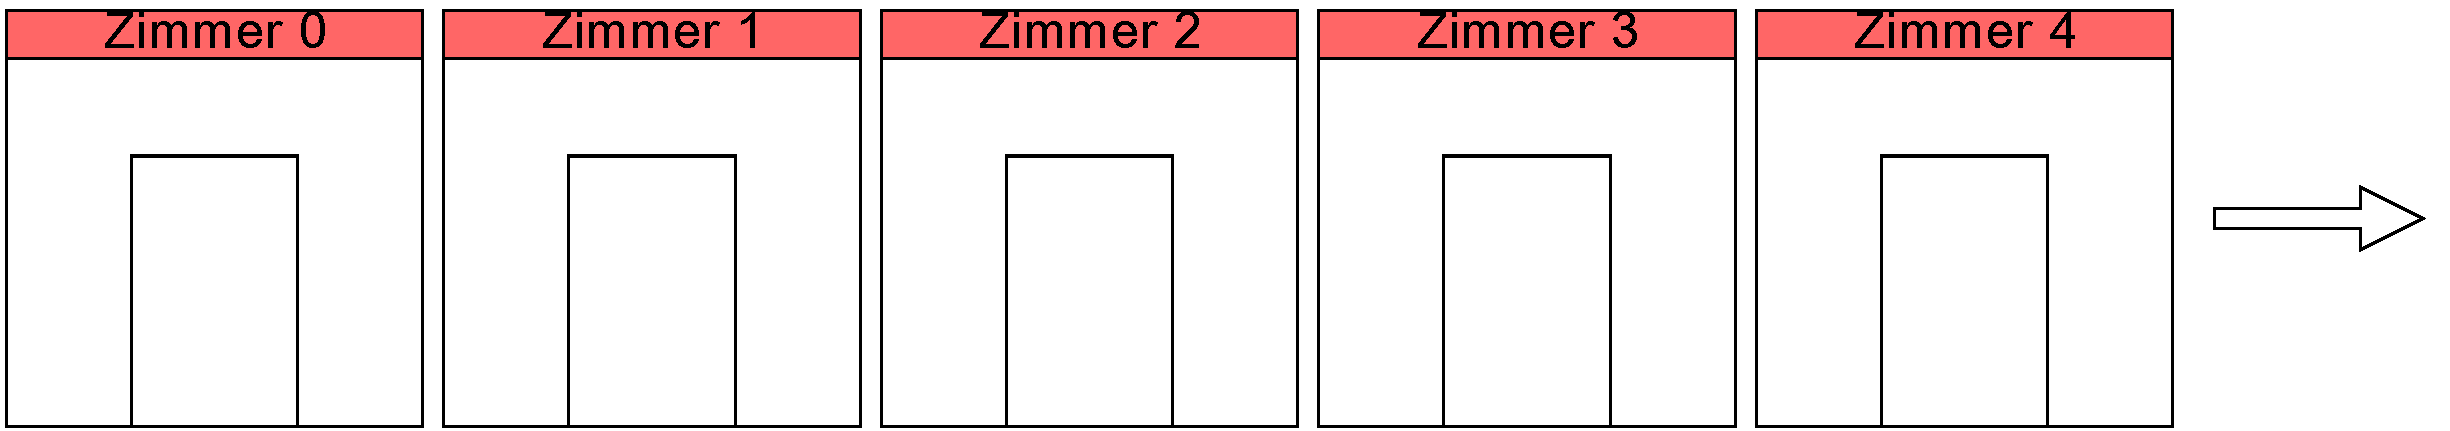
\includegraphics[width=0.9\textwidth]{figures/hilbertHotel}
%\caption*{Hilbert's Hotel}
\end{framed}
\end{center}
Im Rahmen eines Ferienjobs haben Sie eine Stelle als Concierge in Hilbert's Hotel angenommen\footnote{Sie verdienen schliesslich für jedes Zimmer einen Franken pro Arbeitstag.}. An Ihrem ersten Arbeitstag haben Sie die Nachtschicht. Herr Hilbert, der Hotelbesitzer, hat sich bereits zu seinem wohlverdienten Feierabend verabschiedet, als unvermittelt ein älterer Herr (ä.H.) die Lobby betritt.
\begin{itemize}
\item[ä.H.:] Ich bräuchte ein Zimmer in Ihrem Hotel.
\item[Sie:] Es tut mir leid, wir sind voll belegt. Ich könnte Ihnen aber das Hotel ``Cantors Paradise'' empfehlen. Es ist hier ganz in der Nähe, hier steht die Adresse.

\textit{Sie überreichen dem ä.H. eine Visitenkarte vom ``Cantors Paradise''.}
\item[ä.H.:] Mein lieber Concierge, laut Werbebroschüre hat Ihr Hotel unendlich viele Zimmer. Wie soll denn das bitte ausgebucht sein?
\item[Sie:] Na ja, wir haben im Moment unendlich viele Gäste -- in jedem Zimmer einen.
\item[ä.H.:] Das lass ich mal Ihr Problem sein! Mir genügt es, dass hier schwarz auf weiss steht, dass man angeblich keine Reservation zu tätigen braucht, um in diesem Hotel unterzukommen. Zudem werben Sie, mit Bezugnahme auf die Unendlichkeit Ihres Hotels, damit, dass jedem Gast und zu jeder Zeit ein Zimmer garantiert werden kann!

\textit{Der ä.H. kramt genervt seine Werbebroschüre hervor und zeigt sichtlich irritiert auf die entsprechende Seite.}
\item[Sie:] Hmm, ich werde sehen, ob sich da vielleicht doch was machen lässt. Bitte gedulden Sie sich einen Moment.

\textit{Der ä.H. lässt sich auf die grosse Couch fallen, die in der Eingangshalle steht. Sie, nicht ohne ein ziemlich ungutes Gefühl dabei zu haben, wählen Hilberts private Telefonnummer.}
\item[Hi.:] Hilbert am Apparat.
\item[Sie:] Entschuldigen Sie die späte Störung Herr Hilbert. Es ist mir unendlich unangenehm, aber ich habe hier im Hotel ein Problem.
\item[Hi.] Worum geht es denn?
\item[Sie:] Ich habe einen Gast, der trotz Vollbelegung auf ein Zimmer besteht. Und er kann sich erst noch auf unsere eigene Broschüre stützen, in der ja steht, dass wir nie ausgebucht seien, selbst dann nicht, wenn wir mal voll sein sollten!
\item[Hi.:] Ach ja, ich hatte vergessen Sie darauf aufmerksam zu machen. Alle unsere Gäste haben sich beim Bezug ihres Zimmers, {\tiny im Kleingedruckten}, damit einverstanden erklärt, dass wir sie im Notfall ein einziges Mal umplatzieren können. Nutzen Sie diese Klausel um unserem Gast ein Zimmer freizumachen. Noch etwas, machen Sie das Zimmer so frei, dass sie weitere Gäste, die vielleicht später noch kommen, ebenfalls noch unterbringen könnten und bedenken Sie stets, dass jeder Gast höchstens einmal umplatziert werden darf.

\textit{Sie beenden das Gespräch und wenden sich dem ungeduldig wartenden ä.H. zu.}
\item[Sie:] Sehr geehrter Herr, wir haben ein Zimmer für Sie gefunden, sie müssen sich bloss zwei Minuten gedulden, dann können Sie einziehen.
\item[ä.H.:] Sehen Sie, geht doch!
\end{itemize}
Wie bringen Sie den ä.H. unter? Bringen Sie weitere Gäste unter? Was machen Sie, wenn ein voller Limesbus (ein Bus mit unendlich vielen Sitzplätzen) ankommt? Wie lange dauert es bis der ganze Limesbus untergebracht wird?
\end{bsp}

\begin{df}\label{df:endlabzusw}~
\begin{itemize}
\item Eine Menge $X$ heisst \textit{endlich}, falls $X=\varnothing$ oder eine natürliche Zahl $n\geq 1$ und eine bijektive Funktion $f:X \to \{1,\dots,n\}$ existieren.
Ist $X\neq\varnothing$ eine endliche Menge, dann existiert eine Darstellung der Form $X=\{x_1,x_2,\dots,x_n\}$ wobei die Elemente $x_i$ paarweise verschieden sind (d.h. es gilt $i\neq j\Rightarrow x_i\neq x_j$). In diesem Fall hat die Menge $X$ genau $n$ viele Elemente und wir schreiben $|X|=n$. Weiter schreiben wir $|\varnothing| = 0$.
\item Nicht endliche Mengen nennen wir \textit{unendlich}.
\item Eine Menge $X$ heisst \textit{abzählbar}, wenn eine surjektive Funktion $F:\N\to X$ existiert oder wenn $X=\varnothing$ gilt.
\item Die Menge $X$ heisst \textit{abzählbar unendlich}, wenn $X$ abzählbar und unendlich ist.
\item Eine \textit{überabzählbare} Menge ist eine Menge, die nicht abzählbar ist.
\end{itemize}
\end{df}

\begin{rk}\label{rk:abzMengeAnschauung}
Ähnlich wie im Fall von endlichen Mengen ist jede nichtleere abzählbare Menge $X$ von der Form
\[
X=\{a_0,a_1,a_2,\dots \}=\{a_i\mid i\in\N\}.
\]
Den Zusammenhang zu Definition~\ref{df:endlabzusw} liefert hier die Funktion $F:\N\to X$, die durch $F(i)=a_i$ gegeben ist.
\end{rk}
\begin{rk}
Abzählbare Mengen kann man sich auch als die Mengen vorstellen, deren Elemente von den natürlichen Zahlen durchnummeriert  (Wiederholungen erlaubt) werden können. Die Elemente einer abzählbaren Menge lassen sich also in eine Liste schreiben, die für jede natürliche Zahl eine Zeile hat.
\begin{center}
\begin{tabular}{c|c}
$\N$ & $X$\\
\hline
$0$ & $x$\\
$1$ & $y$\\
$2$ & $z$\\
$\vdots$ & $\vdots$
\end{tabular}
\end{center}
\end{rk}

\begin{lm}[Schubfachprinzip]
    Wenn $n$ Objekte auf $m$ Behälter verteilt werden und $n>m$ gilt, dann gibt es mindestens einen Behälter, der mehr als ein Objekt enthält. Formal, sind $n>m$ natürliche Zahlen und gelte $|X|= n$ sowie $|Y|=m$, dann gibt es keine injektive Funktion
    \begin{align*}
    F: X\to Y.
    \end{align*}
\end{lm}

\begin{ueb}~

    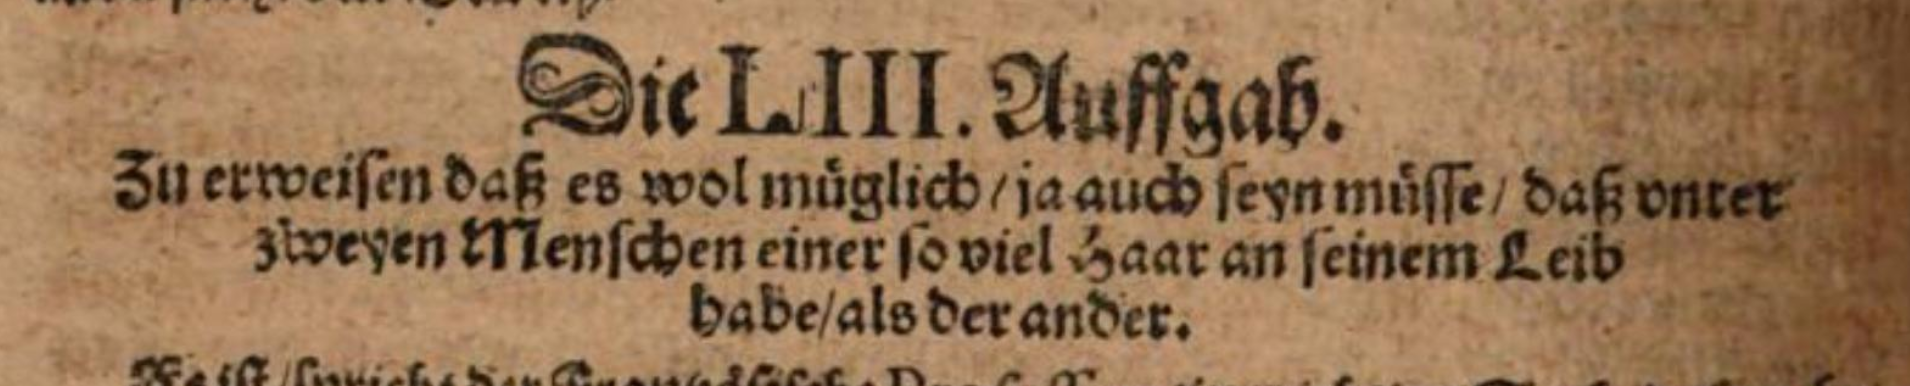
\includegraphics[width=0.9\textwidth]{figures/historicPigeon.png}
\end{ueb}
\begin{lsg}
    \ifthenelse{\boolean{ml}}{
        Wir teilen die Menge aller Menschen wie folgt in Gruppen $G_0,G_1,\dots$ ein
    \begin{align*}
    G_i=\text{ Alle Menschen, die genau $i$ viele Haare am Körper haben.}
    \end{align*}
    Weil jeder Mensch definitiv weniger als $10$ Mio. Haare besitzt (vgl. \url{https://bionumbers.hms.harvard.edu/bionumber.aspx?id=101509}) und weil definitiv mehr als $10$ Mio. Menschen existieren, können wir gemäss dem Schubfachprinzip darauf schliessen, dass es mindestens eine Gruppe mit mehreren Menschen darin gibt (also Menschen mit exakt der gleichen Anzahl an Haaren).
    \vspace{1cm}}{
        ~\answerspace{6cm}
    }
\end{lsg}

\begin{lm}\label{injEndl}
    Gibt es eine injektive Funktion $F:\N\to A$, dann ist die Menge $A$ unendlich.
\end{lm}
\begin{proof}
    Es sei eine Menge $A$ und eine injektive Funktion $F:\N\to A$ gegeben. Wäre die Menge $A$ endlich, dann gäbe es eine natürliche Zahl $n$ mit $|A|=n$. Die Funktion
    \begin{align*}
    G&:\{0,\dots,n\}\to A\\
    G&(x) = F(x)
    \end{align*}
    wäre injektiv und würde, wegen $|\{0,\dots,n\}|=n+1$, dem Schubfachprinzip widersprechen.
\end{proof}

\begin{satz}
    Folgende Aussagen sind für unendliche Mengen $A$ äquivalent:
    \begin{enumerate}
        \item Die Menge $A$ ist abzählbar.
        \item Es gibt eine surjektive Funktion $F_{\N,A}:\N\to A$.
        \item Es gibt eine injektive Funktion $F_{A,\N}:A\to\N$.
        \item Es gibt eine bijektive Funktion $B_{\N,A}:\N\to A$.
        \item Es gibt eine bijektive Funktion $B_{A,\N}:A\to\N$.
    \end{enumerate}
\end{satz}
\begin{proof}~
    \begin{itemize}
        \item Die Aussagen in $a)$ und $b)$ sind per Definition äquivalent.
        \item Die Aussagen in $d)$ und $e)$ sind offensichtlich äquivalent (Umkehrfunktion).
        %\item Für die Implikation $b)\Rightarrow c)$ definieren wir
        %\begin{align*}
        %    F_{A,\N}(a)=\min\{n\in\N \mid F_{\N,A}(n)=a\},
        %\end{align*}
        %dies ist gerechtfertigt\footnote{Wir gehen hier davon aus, dass jede nichtleere Menge von natürlichen Zahlen ein kleinstes Element besitzt, eine Tatsache die wir später beweisen werden.}, da aus der Surjektivität von $F_{\N,A}:\N\to A$ folgt, dass zu jedem $a\in A$ mindestens ein $n\in\N$ mit $F_{\N,A}(n)=a$ existiert. Es bleibt die Injektivität von $F_{A,\N}$ nachzuweisen, dazu nehmen wir $F_{A,\N}(a)=F_{A,\N}(a')$ an. Es folgt, dass es eine natürliche Zahl $n$ mit $F_{\N,A}(n)=a$ und $F_{\N,A}(n)=a'$ gibt. Somit muss wie gewünscht $a=a'$ gelten.
        \item Für die Implikation $c)\Rightarrow b)$, gehen wir von einer injektiven Funktion $F_{A,\N}:A\to\N$ aus.
        Weil diese Funktion injektiv ist, und weil $Dom(F_{A,\N})=A$ gilt, ist
        \begin{align*}
            F_{A,\N}^{-1}:Im(F_{A,\N}) \to A
        \end{align*}
        eine surjektive Funktion. Um eine surjektive Funktion von $\N$ nach $A$ zu erhalten, brauchen wir bloss noch die ``restlichen'' Elemente aus $\N$ zuzuordnen, dazu wählen wir ein beliebiges Element aus $a\in A$ und setzen:
        \begin{align*}
            F_{\N,A}(n)=
                \begin{cases}
                F_{A,\N}^{-1}(n)&\text{falls }n\in Im(F_{A,\N})\\
                a&\text{sonst}
                \end{cases}
        \end{align*}
        \item Für die Implikation $b)\Rightarrow d)$ müssen wir, ausgehend von einer unendlichen Menge $A$ und einer surjektiven Abbildung $F_{\N,A}: \N\to A$, eine bijektive Abbildung $B_{\N,A}: \N\to A$ konstruieren. Da uns für einen vollständigen Beweis die Werkzeuge noch fehlen (Rekursion), wollen wir hier bloss eine Beweisskizze präsentieren. Wir definieren die Funktion $B_{\N,A}$ rekursiv wie folgt:
        \begin{align*}
        B_{\N,A}(0) &= F_{\N,A}(0)\\
        B_{\N,A}(n+1) &= F_{\N,A}(\min\{k\in\N\mid F(k)\neq B_{\N,A}(0),\dots,B_{\N,A}(n) \})
        \end{align*}
        Die resultierende Funktion ist auf ganz $\N$ definiert, weil die Menge $A$ unendlich ist (würde die Rekursion abbrechen, dann wäre $A$ von der Form $\{F_{\N,A}(0),\dots,F_{\N,A}(m)\}$ für ein $m\in\N$). Die Funktion $B_{\N,A}$ ist surjektiv, weil $F_{\N,A}$ surjektiv ist. Die Injektivität folgt, weil per Konstruktion für alle $x,y$
        \begin{align*}
        x<y \Rightarrow B_{\N,A}(x) \neq B_{\N,A}(y)
        \end{align*}
        gilt.
    \end{itemize}
    Weil aus $d)$ und $e)$ alle anderen Aussagen direkt folgen, genügen die gezeigten Implikationen für den Beweis des Satzes.
\end{proof}

\begin{ueb}
    Die Funktion
    \begin{align*}
        &f :\N\to\N\\
        &f(x) =
            \begin{cases}
                \frac{x}{2}&\text{falls $x$ gerade}\\
                3x+1&\text{sonst}
            \end{cases}
    \end{align*}
    Ist surjektiv aber nicht injektiv. Wenn Sie die Funktion so wie im vorhergehenden Beweis im Schritt von $F_1$ zu $B_{\N,A}$ anpassen, welchen Funktionswert erhalten Sie dann für die Eingabe $8$?
\end{ueb}
\begin{lsg}~
    \ifthenelse{\boolean{ml}}{
        $f(9)=28$
    }{
        ~\answerspace{0cm}
    }
\end{lsg}

\begin{bsp}
Die Menge aller geraden natürlichen Zahlen ist abzählbar.
\begin{proof}
Ist $G$ die Menge der geraden Zahlen, dann folgt die Behauptung aus der Tatsache, dass die Funktion
\[
F:\N\to G \phantom{abstand}\text{ mit }\phantom{abstand}F(n)=2n
\]
jede gerade natürliche Zahl trifft (und somit surjektiv ist).
\end{proof}
Dass die Menge der geraden natürlichen Zahlen auch anschaulich abzählbar ist, kann man sich etwa mit folgender Auflistung vergegenwärtigen:
\begin{center}
\begin{tabular}{c|c}
$\N$ & $G$\\
\hline
$0$ & $0$\\
$1$ & $2$\\
$2$ & $4$\\
$\vdots$ & $\vdots$
\end{tabular}
\end{center}
\end{bsp}

\begin{bsp}
Die Menge $\Z$ der ganzen Zahlen ist abzählbar.
\begin{proof}
Wir müssen eine Funktion $F:\N\to\Z$ angeben, die jedes Element von $\Z$ trifft. Dies gelingt uns wie folgt:
\begin{align*}
F(n)=\begin{cases}
-\frac{n}{2} &\text{falls $n$ gerade}\\
\frac{n+1}{2}&\text{falls $n$ ungerade. }
\end{cases}
\end{align*}
\end{proof}
Anschaulich ergibt sich durch die Funktion $F$ folgende Auflistung der ganzen Zahlen:
\begin{center}
\begin{tabular}{c|c}
$\N$ & $\Z$\\
\hline
$0$ & $0$\\
$1$ & $1$\\
$2$ & $-1$\\
$3$ & $2$\\
$4$ & $-2$\\
$5$ & $3$\\
$\vdots$ & $\vdots$
\end{tabular}
\end{center}
\end{bsp}

\begin{bsp}
Die Menge aller \textit{endlichen} Sequenzen der Buchstaben $a,b$ ist abzählbar unendlich. Eine mögliche Auflistung der endlichen Sequenzen ist etwa durch
\begin{center}
\begin{tabular}{c|c}
$\N$ & $X$\\
\hline
$0$ & $a$\\
$1$ & $b$\\
$2$ & $aa$\\
$3$&$ab$\\
$4$&$ba$\\
$5$&$bb$\\
$6$&$aaa$\\
$7$ & $aab$\\
$8$ & $aba$\\
$9$ & $abb$\\
$\vdots$ & $\vdots$
\end{tabular}
\end{center}
gegeben.
\end{bsp}
\begin{bsp}
Die Menge aller Java, C, C\#, C++,Fortran\dots Programme ist abzählbar.
\end{bsp}
\begin{proof}
Wenn jedes Programm mit seinem Bytecode identifiziert wird, dann entspricht jedes Programm einer endlichen $0,1$-Folge. Diese können, gleich wie endliche $a,b$-Sequenzen, abgezählt werden.
\end{proof}
\begin{satz}
Jede endliche Menge ist abzählbar.
\end{satz}
\begin{proof}
Ist $X$ eine endliche Menge, dann können wir $X$ als $\{x_1,\dots,x_n\}$ mit einer natürlichen Zahl $n$ schreiben. Da die leere Menge per Definition abzählbar ist, können wir annehmen, dass $X$ mindestens ein Element $x_1$ besitzt. Wir definieren nun die Funktion $F:\N\to X$ mit
\begin{align*}
F(i)=\begin{cases}
x_i&\text{falls }0<i\leq n\\
x_1&\text{sonst.}
\end{cases}
\end{align*}
Da $F$ offensichtlich jedes Element von $X=\{x_1\dots x_n\}$ trifft, ist $F$ surjektiv. Somit ist $X$ abzählbar.
\end{proof}

\begin{satz}
Jede Teilmenge einer abzählbaren Menge ist abzählbar.
\end{satz}
\begin{proof}
Es sei $X\subseteq Y$ und $Y$ sei eine abzählbare Menge. Da $Y$ abzählbar ist,
gibt es eine surjektive Funktion $F:\N\to Y$. Wenn $X=\varnothing$ gilt, dann
ist $X$ per Definition abzählbar und wir sind fertig. Ist $X\neq\varnothing$,
dann gibt es ein Element $a\in X$. Wir können nun wie folgt eine Abbildung
$G:\N\to X$ angeben.
\begin{align*}
G(x)=\begin{cases}
F(x)&\text{falls }F(x)\in X\\
a&\text{sonst.}
\end{cases}
\end{align*}
Da $X\subseteq Y$ gilt und weil jedes Element von $Y$ von der Funktion $F$
getroffen wird, wird auch jedes Element von $X$ von $G$ getroffen. Somit
ist $G:\N\to X$ surjektiv und $X$ ist also abzählbar.
\end{proof}

\begin{satz}\label{satz:abzaehlbarTransitiv}
Ist $X$ eine abzählbare Menge und gibt es eine surjektive Funktion $F:X\to Y$, dann ist auch $Y$ abzählbar.
\end{satz}
\begin{proof}
Diese Behauptung folgt sofort aus Lemma \ref{lm: komposition inj surj} (die Komposition von surjektiven Funktionen ist wieder surjektiv).
%Sollte $X$ die leere Menge sein, dann ist auch $Y$ leer und somit abzählbar. Ist $X$ nichtleer, dann folgt aus der Abzählbarkeit von $X$, dass es eine surjektive Abbildung $G:\N\to X$ gibt. Wir können nun die Funktion $H:\N\to Y$ durch Komposition der Funktionen $F$ und $G$ bilden, d.h. wir definieren
%\begin{align*}
%H:\N\to Y\phantom{abstand}\text{ mit }\phantom{abstand} H(n)=F(G(n)).
%\end{align*}
%Wir müssen nun noch zeigen, dass wir mit der Funktion $H$ jedes Element von $Y$ treffen. Wir nehmen dazu ein beliebiges Element $y$ von $Y$ und zeigen, dass es eine natürliche Zahl $n$ gibt mit $H(n)=y$. Es sei also $y\in Y$ beliebig. Da die Funktion $F:X\to Y$ surjektiv ist, muss es ein $x\in X$ geben so, dass $F(x)=y$ gilt. Weil aber auch die Funktion $G:\N\to X$ surjektiv ist, muss es ebenfalls eine natürliche Zahl $n$ geben, mit $G(n)=x$. Zusammenfassend können wir also sagen, dass es eine natürliche Zahl und ein Element $x$ aus $X$ gibt, mit der Eigenschaft
%\[
%H(n)=F(G(n))=F(x)=y.
%\]
%Weil $y\in Y$ beliebig gewählt wurde, ist die Funktion $H$ surjektiv.
\end{proof}



\begin{satz}[Erstes Diagonalargument]\label{cantor1}
Die Menge $\N\times\N$, bestehend aus allen Paaren von natürlichen Zahlen, ist abzählbar.
\end{satz}
\begin{proof}[Beweisidee]
Anstelle eines formalen Beweises, skizzieren wir eine Abzählung aller Paare von natürlichen Zahlen wie folgt:
%\begin{figure}[h!]
\begin{center}
\begin{tikzpicture}[scale=1.8]
\node (0) at (0,0) {$(0,0)$};
\node (2) at (0,1) {$(0,1)$};
\node (5) at (0,2) {$(0,2)$};
\node (9) at (0,3) {$(0,3)$};
\node (14) at (0,4) {$(0,4)$};
\node (1) at (1,0) {$(1,0)$};
\node (4) at (1,1) {$(1,1)$};
\node (8) at (1,2) {$(1,2)$};
\node (13) at (1,3) {$(1,3)$};
\node (3) at (2,0) {$(2,0)$};
\node (7) at (2,1) {$(2,1)$};
\node (12) at (2,2) {$(2,2)$};
\node (6) at (3,0) {$(3,0)$};
\node (11) at (3,1) {$(3,1)$};
\node (10) at (4,0) {$(4,0)$};
\draw[->] (0) -- (1);
\draw[->] (1) -- (2);
\draw[->] (2) -- (3);
\draw[->] (3) -- (4);
\draw[->] (4) -- (5);
\draw[->] (5) -- (6);
\draw[->] (6) -- (7);
\draw[->] (7) -- (8);
\draw[->] (8) -- (9);
\draw[->] (9) -- (10);
\draw[->] (10) -- (11);
\draw[->] (11) -- (12);
\draw[->] (12) -- (13);
\draw[->] (13) -- (14);
\end{tikzpicture}
%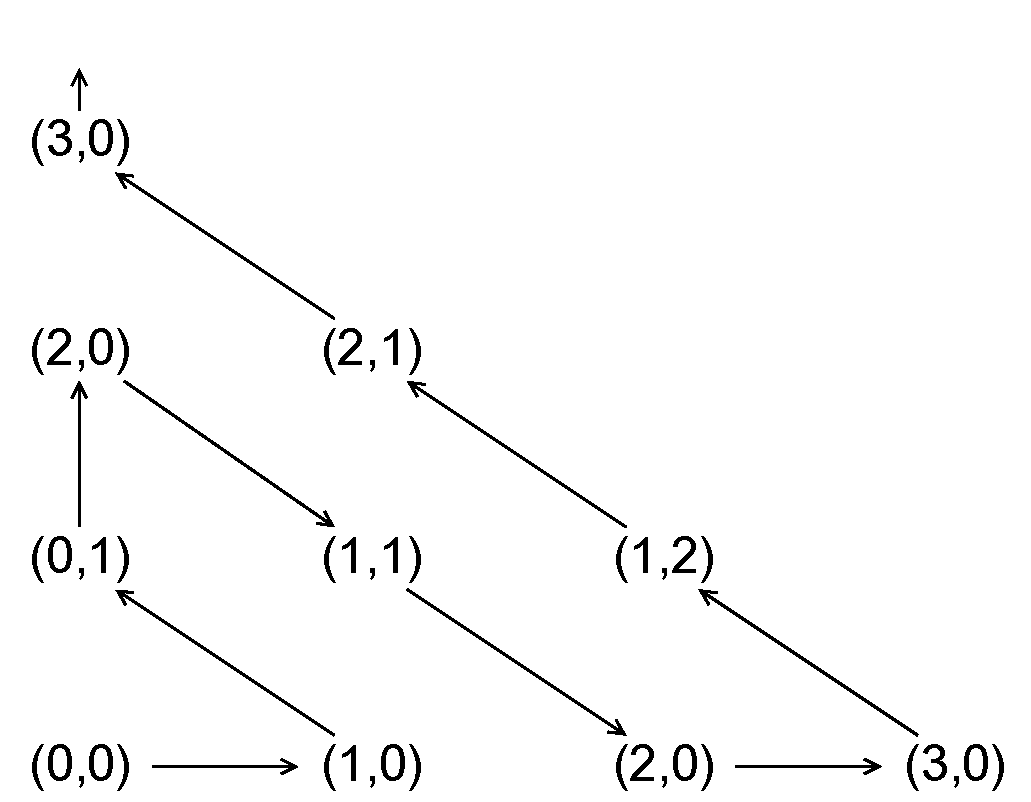
\includegraphics[width=0.5\textwidth]{figures/cantor1}
%\caption*{Die Pfeile deuten die Reihenfolge an, in der die Elemente von $\N\times\N$ abgezählt werden.}
\end{center}
\ %end{figure}
\end{proof}
\begin{satz}\label{satz:countableUnion}
Jede Vereinigung von abzählbar vielen abzählbaren Mengen ist abzählbar. Konkret, jede Vereinigung von der Form
\[
\bigcup_{i\in\N}A_i
\]
ist abzählbar, wenn alle $A_i$'s abzählbar sind.
\end{satz}
\begin{proof}
Wir nehmen an, dass die Menge $\{A_i\mid i\in \N \}$ aus lauter abzählbaren Mengen besteht. Um zu zeigen, dass $\bigcup_{i\in N}A_i$ abzählbar ist, genügt es, aufgrund von Satz~\ref{satz:abzaehlbarTransitiv} und Satz~\ref{cantor1}, zu zeigen, dass es eine surjektive Funktion
\[
H:\N\times\N\to\bigcup_{i\in N}A_i
\]
gibt. Da für jede natürliche Zahl $i$ die Menge $A_i$ abzählbar ist, gibt es für jede natürliche Zahl $i$ auch eine surjektive Funktion $F_i:\N\to A_i$. Wir können die Vereinigungsmenge der $A_i$'s also wie folgt schreiben:
\begin{align*}
\bigcup_{i\in \N}A_i&=\{F_i(j)\mid i,j\in\N \}\\
&=\{F_i(j)\mid (i,j)\in\N\times\N \}.
\end{align*}
Daraus folgt, dass die Funktion
\[
H:\N\times\N\to \bigcup_{i\in N}A_i\phantom{abstand}\text{mit}\phantom{abstand} H(i,j)=F_i(j),
\]
die gesuchte surjektive Funktion ist.
\end{proof}

\begin{cor}
Die Menge $\Z\times \Z$ ist abzählbar.
\end{cor}
\begin{proof}
Wir wissen bereits, dass die Menge $\N\times\N$ abzählbar ist. Daraus folgt, dass auch die Mengen
\begin{align*}
X&=\N\times\{-n\mid n\in \N\}\\
Y&=\{-n\mid n\in \N\}\times\N \\
Z&=\{-n\mid n\in \N\}\times\{-n\mid n\in \N\}
\end{align*}
abzählbar sind. Aus Satz~\ref{satz:countableUnion} folgt also, dass die Menge
\[
\Z\times\Z=(\N\times\N)\cup X\cup Y\cup Z
\]
abzählbar ist.
\end{proof}

\begin{cor}
Die Menge $\Q=\big\{\frac{x}{y}\mid x,y\in \Z\big\}$ der rationalen Zahlen (Brüche) ist abzählbar.
\end{cor}
\begin{proof}
Da die Funktion
\[
F:\Z\times(\Z\setminus{\{0\}})\to \Q\phantom{abstand}\text{mit}\phantom{abstand}F(x,y)=\frac{x}{y}
\]
surjektiv ist, folgt die Behauptung aus Satz~\ref{satz:abzaehlbarTransitiv}.
\end{proof}

\begin{ueb}
Ist die Menge aller endlichen Teilmengen von $\N$ abzählbar? Begründen Sie Ihre Antwort.
\end{ueb}
\begin{lsg}
\ifthenelse{\boolean{ml}}{
Wir können jede endliche Menge von natürlichen Zahlen mittels ihrer charakteristischen Funktion (vgl. Vorlesung) mit einer endlichen Binärsequenz identifizieren. Durch das Hinzufügen einer führenden $1$ zu jeder endlichen Binärsequenz entspricht jede dieser Sequenzen einer natürlichen Zahl in Binärdarstellung. Daraus folgt die Behauptung.}{~\answerspace{7cm}}
\end{lsg}

\begin{thrm}[Zweites Diagonalargument]\label{thrm:cantor2}
Die Menge aller unendlichen Binärsequenzen (Sequenzen aus Nullen und Einsen) ist überabzählbar.
\end{thrm}
\begin{proof}
Beweis durch Widerspruch. Wäre die Menge aller unendlichen Binärsequenzen abzählbar, dann gäbe es eine Liste von der Form\footnote{Natürlich ist die angedeutete Liste Beispielhaft und dient nur der Veranschaulichung unserer Konstruktion der Sequenz $b$. Die Sequenz $s_0$, beispielsweise, könnte auch mit dem Präfix $00000100$ oder irgend einer anderen Folge von Nullen und Einsen beginnen. }
\begin{center}
\begin{tabular}{c|l}
$\N$ & Binärsequenzen\\
\hline
$0$ & $s_0=01101011\cdots$\\
$1$ & $s_1=10010110\cdots$\\
$2$ & $s_2=00101001\cdots$\\
$\vdots$ & $\vdots$
\end{tabular}
\end{center}
in der alle unendlichen Binärsequenzen vorkommen. Wir konstruieren nun, ausgehend von dieser Liste, eine Binärsequenz $b$, die nicht in der Liste enthalten sein kann. Wir definieren $b$ wie folgt:
\begin{align*}
0\text{-tes Glied}&=b(0)=1-s_0(0)\\
1\text{-tes Glied}&=b(1)=1-s_1(1)\\
2\text{-tes Glied}&=b(2)=1-s_2(2)\\
&\vdots\\
n\text{-tes Glied}&=b(n)=1-s_n(n)\\
&\vdots
\end{align*}
Die Folge $b=110\cdots$ kann nicht in der Liste vorkommen, weil sie sich von jedem Element in der Liste in mindestens einem Glied unterscheidet (von der $n$-ten Sequenz unterscheidet sich $b$ im $n$-ten Glied). Dies steht im Widerspruch zu unserer Annahme, dass in der Liste alle unendlichen Binärsequenzen vorkommen.
\end{proof}


\begin{cor}
Das Intervall $(0,1)=\{r\in\R\mid 0<r<1 \}$ ist überabzählbar. Insbesondere ist die Menge $\R$ der reellen Zahlen überabzählbar.
\end{cor}
\begin{proof}
Die reellen Zahlen (in Binärdarstellung) im Intervall $(0,1)$, sind von der Form $0,\dots$ wobei $\dots$ für eine unendliche Binärsequenz steht. Daher steht das Intervall $(0,1)$ mit der Menge aller unendlichen Binärsequenzen in eins-zu-eins Korrespondenz. Die Behauptung folgt daher aus Theorem~\ref{thrm:cantor2}.
\end{proof}

\begin{cor}
Die Potenzmenge von $\N$ ist überabzählbar.
\end{cor}
\begin{proof}
Jede Teilmenge $A$ von $\N$ kann wie folgt durch eine Binärsequenz $\chi_A$ beschrieben werden:
\begin{align*}
\chi_A(n)=\begin{cases}
1&\text{falls } n\in A\\
0&\text{falls} n\notin A.
\end{cases}
\end{align*}
Daher folgt die Behauptung aus Theorem~\ref{thrm:cantor2}.
\end{proof}

\begin{cor}
Die Menge aller Funktionen $F:\N\to\N$ ist überabzählbar.
\end{cor}
\begin{proof}
Die Menge der Binärsequenzen entspricht der Menge der Funktionen $F:\N\to\{0,1\}$. Daher folgt die Behauptung aus Theorem~\ref{thrm:cantor2}.
\end{proof}

\begin{cor}
Es gibt Funktionen $F:\N\to\N$, die von keinem Java, C, C++, Fortran\dots Programm berechenbar sind. Solche Funktionen heissen \textit{unberechenbar}.
\end{cor}


\begin{ueb}
Zeigen Sie, dass die Menge
\[
U=\{1,11,111,1111,\dots \}
\]
aller endlichen Sequenzen von Einsen abzählbar ist. Ist die Menge aller (abzählbar) unendlichen Sequenzen von Einsen auch abzählbar?
\end{ueb}
\begin{lsg}
\ifthenelse{\boolean{ml}}{
	Wir müssen zeigen, dass eine surjektive Abbildung $F:\N\to \{1,11,\dots\}$ existiert. Da dies z.B. für die Funktion
	\begin{align*}
	F(n)=\underbrace{11\dots 1}_{n\text{ viele}}
	\end{align*}
	erfüllt ist, gilt die Behauptung. Die Menge aller (abzählbar) unendlichen $1$-Sequenzen besteht aus nur einem Element und ist somit natürlich abzählbar. }
{~\answerspace{2cm}}
\end{lsg}

\subsection{Ordnungs- und Äquivalenzrelationen}

Neben den Funktionen und ihren Anwendungen gibt es in der Mathematik noch zahlreiche weitere wichtige Klassen von Relationen. Im Folgenden wollen wir auch aufgrund ihrer Wichtigkeit in der Informatik die Ordnungsrelationen (inklusive Halbordnungen) und Äquivalenzrelationen etwas genauer betrachten. Wie viele Typen von Relationen werden auch Ordnungen und Äquivalenzen aufgrund von bestimmten Kombinationen von Grundeigenschaften definiert. Folgend einige wichtige solche Grundeigenschaften.


\begin{df}
    Eine binäre Relation $R$ auf einer Menge $X$ heisst:
    \begin{itemize}
    \item \textit{Reflexiv}, wenn für alle $x\in X$
    \[
    xRx
    \]
    gilt.
    \item \textit{Symmetrisch}, wenn für alle $x,y\in X$
    \[
    xRy\,\Rightarrow\, yRx
    \]
    gilt.
    \item \textit{Antisymmetrisch}, wenn für alle $x,y\in X$
    \[
    xRy\land yRx\,\Rightarrow x=y
    \]
    gilt.
    \item \textit{Transitiv}, wenn für alle $x,y,z\in X$
    \[
    xRy\land yRz\,\Rightarrow \, xRz
    \]
    gilt.
    \end{itemize}
    \end{df}


    \begin{rk}
    Die Relation $R\subseteq X\times X$ ist genau dann reflexiv, wenn die Diagonale
    \[
    \Delta_X:=\{(x,x)\mid x\in X \}
    \]
    eine Teilmenge von $R$ ist. Grafisch heisst das, dass die Diagonale (rot markiert) in $R$ enthalten ist.
    \begin{center}
    \includegraphics[width=0.2\textwidth]{figures/diagonale}
    \end{center}
    Die Relation $R$ ist symmetrisch, wenn ihr Graph symmetrisch bezüglich der Geraden $\Delta_X$ ist.
    \end{rk}


    \begin{bsp}
        Wir betrachten nochmals die Verliebtheitsrelation aus Beispiel \ref{ex:Beispiel1relationen}:
        \[
        pLq:\Leftrightarrow \text{Person $p$ liebt Person $q$.}
        \]
    Die Verliebtheitsrelation hat unter anderem folgende Eigenschaften:
    \begin{itemize}
        \item $L$ ist nicht reflexiv, da nicht alle Menschen ``selbstverliebt'' sind.
        \item $L$ ist (leider\footnote{Andererseits gäbe es wohl keine Literatur oder gar Kunst, wenn diese Relation tatsächlich symmetrisch wäre.}) nicht symmetrisch, da Liebe nicht immer auf Gegenseitigkeit beruht.
        \item $L$ ist nicht Antisymmetrisch, da es durchaus ``echte'' Liebespaare (aus zwei Partnern bestehend) gibt.
        \item $L$ ist nicht transitiv, da die meisten Leute den angebeteten der eigenen angebeteten nicht lieben (ganz im Gegenteil!).
    \end{itemize}
    \end{bsp}

    \begin{ueb}
        Geben Sie binäre Relationen (auf der Menge aller Menschen) mit folgenden Eigenschaften an:
        \begin{enumerate}
            \item Transitiv und nicht antisymmetrisch.
            \item Transitiv, reflexiv und antisymmetrisch.
            \item Nicht reflexiv, nicht transitiv.
        \end{enumerate}
    \end{ueb}
    \begin{lsg}
        \ifthenelse{\boolean{ml}}{
            Zum Beispiel:
            \begin{enumerate}
                \item $pJq:\Leftrightarrow $ Person $p$ ist jünger oder gleichalt (in Jahren) wie Person $q$.
                \item $pWq:\Leftrightarrow$ Person $p$ ist echt jünger als Person $q$.
                \item $pGq:\Leftrightarrow$ Person $p$ ist vom anderen Geschlecht als Person $q$.
            \end{enumerate}
            }{~
            \answerspace{5cm}
            }
    \end{lsg}


    \subsection*{Äquivalenzrelationen}

    Äquivalenzrelationen sind in einem gewissen Sinn (konkret im Sinn von Satz~\ref{satz: equivalenzen verallgemeinerte gleichheit}) verallgemeinerte Gleichheitsrelationen. Sie werden dazu verwendet, (im Sinn der Relation) ähnliche Objekte miteinander zu identifizieren und als ``gleich'' zu behandeln.

    \begin{df}
    \textit{Äquivalenzrelationen} sind reflexive, symmetrische und transitive Relationen.
    \end{df}

    \begin{bsp}
    Auf jeder Menge $X$ ist die Gleichheitsrelation $\Delta_X=\{(x,x)\mid x\in X \}$ eine Äquivalenzrelation. Weil jede Äquivalenzrelation reflexiv ist, ist die Gleichheitsrelation auf jeder Menge die ``kleinste'' Äquivalenzrelation. Am anderen Ende des Spektrums steht die Relation $X\times X$, sie ist die grösste Äquivalenzrelation auf der Menge $X$.
    \end{bsp}

    \begin{bsp}
    Von den Relationen $R_1,R_2,R_3$ und $T$ aus Beispiel~\ref{ex:Beispiel1relationen}, sind $R_1,R_2$ Äquivalenzrelationen.
    \begin{itemize}
    \item Die Relation $R_3$ ist keine Äquivalenzrelation, weil sie nicht reflexiv (nicht jeder liebt sich selbst), nicht symmetrisch (es gibt unglücklich Verliebte) und nicht transitiv ist. Man beachte, dass jeder einzelne der genannten Gründe genügt, damit $R_3$ keine Äquivalenzrelation ist.
    \item Die Relation $T$ ist zwar reflexiv und transitiv, aber nicht symmetrisch und daher auch keine Äquivalenzrelation.
    \end{itemize}
    \end{bsp}


    \begin{df}
    Es sei $R$ eine Äquivalenzrelation auf einer Menge $X$ und $x\in X$. Die \textit{Äquivalenzklasse} $[x]_R$ von $x$ bezüglich $R$ ist die Menge aller Elemente von $X$, die zu $x$ in Relation $R$ stehen:
    \[
    [x]_R:=\{y\in X\mid xRy \}
    \]
    Jedes Element einer Äquivalenzklasse nennen wir einen \textit{Repräsentanten} der entsprechenden Äquivalenzklasse. Die \textit{Faktormenge} $\faktor{X}{R}$ \textit{von} $X$ \textit{modulo} $R$ ist die Menge aller Äquivalenzklassen:
    \[
    \faktor{X}{R}:=\big\{ [x]_R\mid x\in X \big\}
    \]
    \end{df}

    \begin{bsp}\label{bsp:modulo5relation}
    Wir betrachten die Relation $\equiv_5$ auf der Menge $\Z$, die wie folgt gegeben ist:
    \[
    x\equiv_5 y:\Leftrightarrow (x-y)\text{ ist ein Vielfaches von  }5.
    \]
    Als Java Code könnte man die Relation auch wie folgt darstellen:

    \begin{framed}
        \begin{lstlisting}{static,boolean}
    static boolean Rel(int x, int y){
        if (y<0) return Rel(x,y+5);
        if (x<0) return Rel(x+5,y);
        if (y>=5) return Rel(x,y-5);
        if (x>=5) return Rel(x-5,y);
        return x == y;
    }
    \end{lstlisting}
    \end{framed}
    Wir überzeugen uns nun davon, dass diese Relation eine Äquivalenzrelation ist.
    \begin{itemize}
    \item \textbf{Reflexivität}: Es gilt für jede ganze Zahl $z$
    \[
    0\cdot 5=0=(z-z).
    \]
    Also ist $(z-z)$ ein Vielfaches von $5$, somit gilt $z\equiv_5 z$.
    \item\textbf{Symmetrie}: Gilt $x\equiv_5 y$, dann gibt es eine ganze Zahl $z$ mit $5z=(x-y)$. Also ist auch
    \[
    (y-x)=-(x-y)=-5z=5\cdot(-z)
    \]
    ein Vielfaches von $5$, d.h. es gilt $y\equiv_5x$.
    \item\textbf{Transitivität}: Gilt $x\equiv_5 y$ und $y\equiv_5 z$, dann gibt es ganze Zahlen $r,s$ mit $5r=x-y$ und $5s=y-z$. Insgesamt erhalten wir, dass
    \[
    x-z=(x-y)+(y-z)=5r+5s=5(r+s)
    \]
    ein Vielfaches von $5$ ist und somit, dass $x\equiv_5 z$ gilt.
    \end{itemize}
    Wir betrachten nun die Äquivalenzklassen modulo der Relation $\equiv_5$ (diese heissen Restklassen modulo $5$).
    \begin{align*}
    [0]_{\equiv_5}&=\{x\in \Z\mid 0\equiv_5y \}\\ &=\{z\in\Z\mid z\text{ ist ein Vielfaches von }5 \}\\
    &=\{5z\mid z\in\Z \}\\
    \phantom{dd}\\
    [1]_{\equiv_5}&=\{x\in \Z\mid 1\equiv_5y \}\\ &=\{z\in\Z\mid \text{ Bei Division durch }5\text{ lässt }z\text{ den Rest }1 \}\\
    &=\{5z+1\mid z\in\Z\}\\
    \phantom{dd}\\
    [2]_{\equiv_5}&=\{x\in \Z\mid 2\equiv_5y \}\\ &=\{z\in\Z\mid \text{ Bei Division durch }5\text{ lässt }z\text{ den Rest }2 \}\\
    &=\{5z+2\mid z\in\Z\}\\
    \phantom{dd}\\
    [3]_{\equiv_5}&=\{x\in \Z\mid 3\equiv_5y \}\\ &=\{z\in\Z\mid \text{ Bei Division durch }5\text{ lässt }z\text{ den Rest }3 \}\\
    &=\{5z+3\mid z\in\Z\}\\
    \phantom{dd}\\
    [4]_{\equiv_5}&=\{x\in \Z\mid 4\equiv_5y \}\\ &=\{z\in\Z\mid \text{ Bei Division durch }5\text{ lässt }z\text{ den Rest }4 \}\\
    &=\{5z+4\mid z\in\Z\}
    \end{align*}
    Die Faktormenge der Relation $\equiv_5$ ist also durch
    \[
    \faktor{\Z}{\equiv_5}=\{ [0]_{\equiv_5},[1]_{\equiv_5},[2]_{\equiv_5},[3]_{\equiv_5},[4]_{\equiv_5} \}
    \]
    gegeben.
    \end{bsp}
    \begin{lm}\label{lm:sim gleiche klasse}
    Ist $\sim $ eine Äquivalenzrelation auf einer Menge $X$ und gilt $x,y\in X$ mit $x\sim y$, dann gilt $[x]_\sim=[y]_\sim$. Mit anderen Worten, äquivalente Elemente repräsentieren stets dieselbe Äquivalenzklasse.
    \end{lm}
    \begin{proof}
    Seien $X,\sim,x,y$ wie in der Behauptung. Um zu zeigen, dass $[x]_\sim=[y]_\sim$ gilt, genügt es nachzuweisen, dass $x\sim z\Leftrightarrow y\sim z$ für beliebige $z\in X$ gilt. Wir nehmen $x\sim y$ an, dann gilt
    \begin{align*}
    y\sim z\Rightarrow x\sim y\land y\sim z \stackrel{\text{Transitivität}}{\Longrightarrow} x\sim z
    \end{align*}
    und
    \[
    x\sim z\Rightarrow x\sim y\land x\sim z\stackrel{\text{Symmetrie}}{\Longrightarrow} y\sim x\land x\sim z\stackrel{\text{Transitivität}}{\Longrightarrow} y\sim z,
    \]
    wie gewünscht.
    \end{proof}
    \begin{cor}\label{cor:alle Elemente Repräsentanten}
    Ist $\sim $ eine Äquivalenzrelation auf $X$ und sind $x,y\in X$ mit $x\in[y]_\sim$, dann gilt $[x]_\sim=[y]_\sim$. Mit anderen Worten, jedes Element einer Äquivalenzklasse ist auch ein Repräsentant dieser Äquivalenzklasse.
    \end{cor}
    \begin{proof}
    Es seien $X,\sim,x$ und $y$ wie in der Behauptung. Aus $x\in[y]_\sim$ folgt $y\sim x$. Die Behauptung folgt nun aus Lemma~\ref{lm:sim gleiche klasse}.
    \end{proof}

    \begin{satz}\label{satz: equivalenzklassen disjunkt}
    Ist $\sim $ eine Äquivalenzrelation auf $X$ und sind $x,y\in X$ mit $[x]_\sim\neq[y]_\sim$, dann gilt $[x]_\sim\cap[y]_\sim=\varnothing$.
    Mit anderen Worten, verschiedene Äquivalenzklassen sind immer disjunkt.
    \end{satz}
    \begin{proof}
    Es seien $X,\sim,x$ und $y$ wie in der Behauptung. Wir zeigen die Kontraposition, d.h.
    \[
    [x]_\sim\cap[y]_\sim\neq\varnothing\Rightarrow [x]_\sim=[y]_\sim.
    \]
    Es gelte also $[x]_\sim\cap[y]_\sim\neq\varnothing$, es gibt daher ein $z\in [x]_\sim\cap[y]_\sim$. Daraus folgt, dass $x\sim z\land y\sim z$ gilt und wegen der Transitivität und der Symmetrie von $\sim$ folgt sofort $x\sim y$. Die Behauptung folgt nun aus Lemma~\ref{lm:sim gleiche klasse}.
    \end{proof}


    \begin{satz}\label{satz: equivalenzklassen partition}
    Ist $\sim$ eine Äquivalenzrelation auf einer Menge $X$, dann ist die Faktormenge $\faktor{X}{\sim}$ eine Partition von $X$.
    \end{satz}
    \begin{proof}
    Es sei $\sim$ eine beliebige Äquivalenzrelation auf einer Menge $X$. Wir müssen folgende Punkte verifizieren:
    \begin{enumerate}
    \item\label{a} Die Äquivalenzklassen sind alle nichtleer.
    \item\label{2} Die Äquivalenzklassen sind paarweise disjunkt.
    \item\label{3} Es gilt
    \[
    \bigcup_{x\in X}[x]_{\sim}=X.
    \]
    \end{enumerate}
    Der erste Punkt folgt aus der Definition von der Faktormenge (die Äquivalenzklassen sind via ihrer Repräsentanten definiert). Die Tatsache, dass die Äquivalenzklassen paarweise disjunkt sind, ist genau die Aussage von Satz~\ref{satz: equivalenzklassen disjunkt}. Wir brauchen also bloss noch den letzten Punkt zu verifizieren. Dies folgt, da für jedes $z\in X$, wegen der Reflexivität, $z\sim z$ und somit
    \[
    z\in[z]_\sim\subseteq\bigcup_{x\in X}[x]_\sim
    \]
    gilt.
    \end{proof}

    \begin{rk}
        Das Konzept von Äquivalenzklassen (und deren Zusammenhang mit Partitionen) werden Sie in der theoretischen Informatik in Form von sogenannten ``Zustandsklassen'' wiederfinden, diese werden dort gebraucht, um zu zeigen, dass es Sprachen gibt, die nicht mit ``endlichen Zustandsautomaten'' erkannt werden können.
    \end{rk}

    \begin{ueb}\label{greg}
        Gegeben Sei die Äquivalenzrelation
        \[
            pRq:\Leftrightarrow\text{$p$ hat am gleichen Tag Geburtstag wie $q$.}
        \]
        Kommentieren Sie folgende Aussagen mit ``wahr'', ``falsch'' oder ``unklar'' unter der
        Annahme $Ray\, R\, Greg $:
        \begin{enumerate}
            \item Ray ist älter als Greg oder Greg ist älter als Ray.
            \item Ray und Greg sind gleich alt.
            \item Ray ist verwandt mit Greg.
            \item Der Altersunterschied von Ray und Greg in Jahren ist ganzzahlig.
        \end{enumerate}
    \end{ueb}
    \begin{lsg}
        \ifthenelse{\boolean{ml}}{
            $d)$ ist wahr, die restlichen Aussagen sind aufgrund der Annahmen nicht entscheidbar.}
            {~
                \answerspace{2cm}}
    \end{lsg}

    \begin{ueb}
        Wie viele Äquivalenzklassen hat die Relation $R$ von Übung \ref{greg}?
    \end{ueb}
    \begin{lsg}
        \ifthenelse{\boolean{ml}}{
            $366$ (Auch in Schaltjahren haben an jedem Tag Leute Geburtstag.)}{~
            \answerspace{1cm}}
    \end{lsg}

    Wir haben in Satz~\ref{satz: equivalenzklassen partition} gesehen, dass jede 	Äquivalenzrelation auf einer Menge eine Partition auf eben dieser Menge induziert. Als Nächstes sehen wir, dass auch die Umkehrung gilt; jede Partition induziert eine Äquivalenzrelation, deren Faktormenge genau der ursprünglichen Partition entspricht. Insgesamt sehen wir, dass eine eins-zu-eins Korrespondenz zwischen allen möglichen Partitionen und allen möglichen Äquivalenzrelationen auf einer gegebenen Menge existiert.

    \begin{satz}
    Ist $P=\{A_i\mid i\in I\}$ eine Partition von der Menge $X$, dann ist die Relation $\sim$, gegeben durch
    \[
    x\sim y:\Leftrightarrow \exists i\in I\,(x\in A_i\land y\in A_i),
    \]
    eine Äquivalenzrelation auf $X$. Zusätzlich gilt
    \[
    \faktor{X}{\sim}=P.
    \]
    \end{satz}
    \begin{proof}
    Zuerst zeigen wir, dass die Relation $\sim$ unter den gegebenen Umständen eine Äquivalenzrelation ist.
    \begin{itemize}
    \item \textbf{Reflexivität}: Sei $x\in X$  beliebig. Wir müssen zeigen, dass $x\sim x$ gilt. Da $P=\{A_i\mid i\in I\}$ eine Partition von $X$ ist, gibt es ein $i\in I$ mit $x\in A_i$, daraus folgt sofort $x\sim x$.
    \item \textbf{Symmetrie}: Es gelte $x\sim y$. Wir müssen $y\sim x$ zeigen. Aus $x\sim y$ folgt, dass es ein $i\in I$ mit $x\in A_i\land y\in A_i$ gibt, dies ist offensichtlich äquivalent zu $y\sim x$.
    \item \textbf{Transitivität}: Es gelte $x\sim y\land y\sim z$. Wir müssen $x\sim z$ zeigen. Aus $x\sim y\land y\sim z$ folgt, dass es $i,j\in I$ gibt so, dass $x,y\in A_i$ und $y,z\in A_j$ gilt. Da $P=\{A_i\mid i\in I\}$ eine Partition ist, kann $y $ nicht in zwei verschiedenen Blöcken enthalten sein, es gilt daher $i=j$ und somit $x\sim z$.
    \end{itemize}
    Dass die Äquivalenzklassen von $\sim$ genau den Blöcken von $P$ entsprechen ist sofort klar, wenn man beachtet, dass zwei Elemente genau dann äquivalent sind, wenn sie im selben Block von $P$ liegen.
    \end{proof}

    Am Anfang dieses Abschnittes haben wir Äquivalenzrelationen als verallgemeinerte Gleichheitsrelationen beschrieben, dies können wir im folgenden Satz präzisieren.

    \begin{satz}\label{satz: equivalenzen verallgemeinerte gleichheit}
    Für jede Relation $\sim$ auf einer Menge $X$ sind folgende beiden Aussagen äquivalent.
    \begin{enumerate}
    \item[1.] Die Relation $\sim$ ist eine Äquivalenzrelation.
    \item[2.] Es gibt eine Menge $Y$ und ein Funktion $F:X\to Y$ so, dass für alle $x,y\in X$
    \[
    x\sim y\Leftrightarrow F(x)=F(y)
    \]
    gilt.
    \end{enumerate}
    \end{satz}
    \begin{proof}
    Wenn $\sim$ eine Äquivalenzrelation auf der Menge $X$ ist, dann erfüllt die Abbildung
    \[
    F:X\to\mathcal{P}(X)\phantom{abstand}\text{mit} \phantom{abstand} F(x)=[x]_\sim
    \]
    alle geforderten Eigenschaften. Ist umgekehrt eine Funktion $F:X\to Y$ wie in der Behauptung gegeben, dann gilt für die Relation $\sim$ Folgendes:
    \begin{itemize}
    \item\textbf{Reflexivität} gilt, da für jedes Element $x\in X$ trivialerweise $F(x)=F(x)$ gilt.
    \item \textbf{Symmetrie} folgt, da für beliebige Elemente $x,y\in X$
    \[
    x\sim y\Rightarrow F(x)=F(y)\Rightarrow F(y)=F(x)\Rightarrow y\sim x
    \]
    gilt.
    \item\textbf{Transitivität} folgt, da für beliebige Elemente $x,y,z\in X$
    \[
    x\sim y\land y\sim z\Rightarrow F(x)=F(y)\land F(y)=F(z)\Rightarrow F(x)=F(z)\Rightarrow  x\sim z
    \]
    gilt.
    \end{itemize}
    \end{proof}



    \begin{bsp}
    Es sei $\sim_{14}$ die folgendermassen auf der Menge $Fun(\R)=\{F\mid F:\R\to\R\}$ gegebene Relation:
    \[
    F\sim G:\Leftrightarrow F(14)=G(14).
    \]
    Wir betrachten die Funktion
    \[
    Eval_{14}:Fun(\R)\to \R\phantom{abstand}\text{mit}\phantom{abstand}Eval_{14}(F)=F(14).
    \]
    Offenbar gilt
    \[
    F\sim_{14}G\Leftrightarrow Eval_{14}(F)=Eval_{14}(G).
    \]
    Anhand von Satz~\ref{satz: equivalenzen verallgemeinerte gleichheit} sehen wir also sofort, dass es sich bei $\sim_{14}$ um eine Äquivalenzrelation handelt.
    \end{bsp}

    \begin{rk}[Wohldefiniertheitsproblem]
    Wir betrachten die Relation $\simeq$, die auf der Menge $\N$ folgendermassen gegeben ist.
    \[
    n\simeq m\Leftrightarrow n,m\text{ haben die gleichen Primteiler}.
    \]
    Nun definieren wir eine Funktion
    \[
    F:\faktor{\N}{\simeq}\to \N\phantom{abstand}F([x]_\simeq):=x+102.
    \]
    Es soll zum Beispiel $F([7]_\simeq)=109$ gelten. Sehen Sie ein Problem bei unserem Vorgehen? Ist $F([49]_\simeq)=151$? Es gilt doch $7\simeq 49$ und somit auch $[7]_\simeq=[49]_\simeq$. Sollte dann nicht auch $F([7]_\simeq)=F([49]_\simeq)$ gelten? Natürlich schon! Das Problem, das wir hier haben, nennt man ein \textit{Wohldefiniertheitsproblem}. Es entsteht, wenn man Funktionswerte von Äquivalenzklassen mit Bezugnahme auf deren Repräsentanten definiert, ohne sicherzustellen, dass der Funktionswert nicht von der Wahl der Repräsentanten abhängt.

    Sind eine Äquivalenzrelation $\sim$ auf einer Menge $X$ und eine Funktion $F:X\to Y$ gegeben, so erhält man nur dann durch die Zuordnung
    \[
    \tilde F([x]_\sim):=F(x)
    \]
    eine wohldefinierte Funktion
    \[
    \tilde F:\faktor{X}{\sim}\to Y,
    \]
    wenn die Funktion $F$ mit der Relation $\sim$ verträglich ist. Das heisst, wenn
    \[
    x\sim y\Rightarrow F(x)=F(y)
    \]
    gilt.
    \end{rk}

    \begin{bsp}
    Ein Beispiel (vgl.~\ref{bsp:modulo5relation}) für eine wohldefinierte Abbildung
    \[
    F:\faktor{\Z}{\equiv_5}\to\faktor{\Z}{\equiv_5}
    \]
    erhalten wir z.B. durch die Zuordnung
    \[
    F([x]_{\equiv_5}):=[2x+3]_{\equiv_5}.
    \]
    Um zu sehen, dass diese Funktion tatsächlich wohldefiniert ist, betrachten wir:
    \begin{align*}
    x\equiv_5 y&\Rightarrow (x-y)\text{ ist Vielfaches von } 5\\
    &\Rightarrow\exists z\in\Z\,(5z=x-y)\\
    &\Rightarrow \exists z\in\Z\,\big((2x+3)-(2y+3)=2x-2y=2(x-y)=5(2z)\big)\\
    &\Rightarrow (2x+3)-(2y+3)\text{ ist ein Vielfaches von }5\\
    &\Rightarrow [2x+3]_{\equiv_5}=[2y+3]_{\equiv_5}\\
    \end{align*}
    \end{bsp}


    \subsection*{Ordnungsrelationen}

    Unter Ordnungsrelationen fasst man alle Arten von Relationen zusammen, mithilfe derer man
    Objekte in gewisser Weise vergleichen und mehr oder weniger eindeutig sortieren kann. Das
    Standardbeispiel ist die Ordnungsrelationen $\leq$ auf den verschiedenen Zahlenmengen.

    \begin{df}\label{df:minimale elemente}
    Es sei $R$ eine binäre Relation auf der Menge $M$.
    \begin{itemize}
    \item Zwei Elemente $x,y\in M$ heissen $R$-\textit{unvergleichbar}, falls weder $xRy$ noch $yRx$ gilt.
    \item Ein Element $x\in X$ einer Teilmenge $X\subseteq M$ von $M$ heisst $R$-\textit{minimal in $X$}, falls es kein anderes Element $y\in X$ mit $yRx$ gibt.
    \item  Ein Element $x\in X$ einer Teilmenge $X\subseteq M$ von $M$ heisst $R$-\textit{maximal in $X$}, falls es kein anderes Element $y\in X$ mit $xRy$ gibt.
    \end{itemize}
    Wenn keine Missverständnisse zu befürchten sind, dann schreiben wir anstelle von $R$-minimal, $R$-maximal und $R$-unvergleichbar auch einfach minimal, maximal und unvergleichbar.
    \end{df}

    \begin{ueb}
        Es sei $R$ die Gleichheitsrelation auf der Menge der natürlichen Zahlen. Welches sind die $R$-minimalen und $R$-maximalen Elemente?
    \end{ueb}
    \begin{lsg}~
        \ifthenelse{\boolean{ml}}{
            Alle natürlichen Zahlen sind sowohl minimal als auch maximal bezüglich der Gleichheitsrelation.
            }{~
            \answerspace{0cm}
            }
    \end{lsg}

    \begin{rk}
        Es sei $X$ eine Teilmenge von $M$ und $R$ eine binäre Relation auf $M$.
        Die $R$-minimalen Elemente von $X$ entsprechen im Graph $G=(M,R)$ genau den Knoten, bei
        denen keine Pfeile enden, die ihren Ursprung in $X$ haben. Die maximalen Elemente
        entsprechen den Knoten, von denen alle ausgehenden Pfeile aus der Menge $X$
        ``hinauszeigen''. Zwei Elemente $x,y\in M$ sind $R$-unvergleichlich, wenn es keine
        Pfeile (egal in welcher Richtung) gibt, die $x$ und $y$ verbinden.
    \end{rk}

    \begin{ueb}
    Die Relation $R$ auf der Menge $M=\{a,b,u,v,x,y,z\}$ sei durch den Graph $(M,R)$ wie folgt
    gegeben.
    \begin{center}
    \includegraphics[width=0.5\textwidth]{graphviz/maxmingraph}
    \end{center}
    Geben Sie alle minimalen und maximalen Elemente von $M$ an. Geben Sie weiter zwei Elemente an, die unvergleichbar sind.
    \end{ueb}
    \begin{lsg}~
    \ifthenelse{\boolean{ml}}{
        \begin{itemize}
            \item Die minimalen Elemente von $M$ sind $a$ und $x$.
            \item Das einzige maximale Elemente von $M$ ist $z$.
            \item Die Elemente $a$ und $x$ sind z.B. unvergleichbar.
        \end{itemize}
        }{~
        \answerspace{4cm}}
    \end{lsg}

    \begin{df}
    Es sei $R$ eine binäre Relation auf der Menge $M$.
    \begin{itemize}
    \item $R$ ist eine \textit{Präordnung} auf $M$, wenn $R$ reflexiv und transitiv ist.
    \item $R$ ist eine \textit{Halbordnung} auf $M$, wenn $R$ reflexiv, antisymmetrisch und transitiv ist.
    \item $R$ ist eine \textit{totale oder lineare Ordnung} auf $M$, wenn $R$ eine Halbordnung ist und keine $R$-unvergleichbaren Elemente existieren.
    \item $R$ ist eine \textit{Wohlordnung} auf $M$, wenn $R$ eine totale Ordnung auf $M$ ist so, dass jede Teilmenge $X\neq\varnothing$ von $M$ (mindestens) ein $R$-minimales Element enthält.
    \end{itemize}
    \end{df}


    \begin{bsp}~
    \begin{itemize}
    \item Die Relation $\leq$ auf der Menge $\R$ ist eine totale Ordnung, die aber keine Wohlordnung ist (die Menge $\{x\in\R\mid 0<x<1\}$ hat kein kleinstes Element). Auf der Menge $\N$ ist $\leq$ eine Wohlordnung\footnote{Ein Beweis dazu kommt im nächsten Kapitel.}. Auf der Menge $\Z$ ist die Relation $\leq$ keine Wohlordnung. Wieso?
    \item Ist $A$ eine Menge von Mengen, dann ist die Teilmengenrelation $\subseteq$ eine Halbordnung.
    \item Die Teilerrelation $T$ auf der Menge $\Z$ ist eine Halbordnung aber keine totale Ordnung. Die Elemente $7$ und $5$ sind $T$-unvergleichlich.
    \end{itemize}
    \end{bsp}

    \begin{df}
        Es sei $R$ eine (bin\"are) Relation.
        \begin{itemize}
            \item Als \textit{transitiven Abschluss} von $R$ bezeichnet man die kleinste
            (bezüglich $\subseteq$) transitive Relation, die $R$ als Teilmenge enthält,
            sie wird mit $R^+$ notiert.
            \item Die kleinste Relation, die $R^+$ enthält und reflexiv ist, nennt man den
            \textit{reflexiv-transitiven Abschluss} von $R$, sie wird mit $R^*$ bezeichnet.
        \end{itemize}
    \end{df}

    \begin{rk}
        F\"ur eine beliebige (bin\"are) Relation $R$ gilt genau dann $xR^*y$, wenn es
        eine endliche Folge $x=k_1,\dots,k_n=y$ gibt, so dass $k_iRk_{i+1}$ f\"ur alle
        Indices $i=1,\dots,n-1$ gilt. Es gilt also genau dann $xR^*y$, wenn es eine Folge von
        Elementen gibt, die mit $x$ beginnt, mit $y$ endet und deren Elemente alle der Reihe
        nach in Relation $R$ zueinander stehen. Ist $G=(V,E)$ ein Graph, dann bedeutet
        $xE^*y$, dass in $G$ ein Pfad von $x$ nach $y$ existiert.
    \end{rk}

    \begin{df}
        Ein \textit{Weg} oder \textit{Pfad} in einem Graph $G=(V,E)$ ist eine endliche Folge
        $k_1,\dots,k_n\in V$ von Knoten, so dass $k_iEk_{i+1}$ f\"ur alle Indices
        $i=1,\dots,n-1$ gilt. Die Knoten $k_1$ und $k_n$ bezeichnet man als \textit{Anfangs-}
        und \textit{Endpunkt} des Pfades. Gilt zusätzlich $k_1=k_n$, dann spricht man von einem \textit{Zyklus}.
    \end{df}


    \begin{rk}
        In der Informatik wichtige Datenstrukturen sind sogenannte \textit{DAGs} (von ``directed acyclic graph''), gerichtete zyklenfreie Graphen. Eine der charakteristischen Eigenschaften von DAG's ist die Tatsache, dass sich ihre Elemente auf eine mit der Struktur des Graphen verträgliche Art sortieren lassen. Oft werden Abhängigkeiten von einzelnen Arbeitsschritten eines Prozesses als DAG modelliert, eine mit der Struktur des Graphen verträgliche lineare Ordnung der Knoten entspricht dann einer möglichen Reihenfolge in der die einzelnen Arbeitsschritte abgearbeitet werden können (ohne Abhängigkeiten zu verletzen).
    \end{rk}


    \begin{df}
        Es sei $M$ eine endliche Menge und $G=(M,E)$ ein DAG. Eine lineare Ordnung $\preceq\subseteq M\times M$ ist eine \textit{topologische Sortierung} von $G$, wenn für alle $a,b\in M$
        \begin{align*}
        a E^* b  \Rightarrow a\preceq b
        \end{align*}
        gilt.
    \end{df}

    \begin{satz}~
        Jeder endliche DAG besitzt (mindestens) eine topologische Sortierung.
    \end{satz}
    \begin{proof}
        Wir bemerken zuerst, dass jeder endliche DAG $G=(V,E)$ minimale Elemente bezüglich der Relation $E$ besitzt (wieso?). Weiter bemerken wir, dass jeder DAG, von dem ein minimaler Knoten (zusammen mit den von diesem Knoten ausgehenden Pfeilen) entfernt wird, wieder ein DAG ist (entfernen von Knoten und Verbindungen kann keine neuen Zyklen erzeugen). Aus diesen Beobachtungen folgt, dass folgender Algorithmus eine topologische Sortierung für jeden endlichen DAG generiert:
        \begin{enumerate}
            \item Wenn $G=(V,E)$ nicht leer ist, dann wähle ein bezüglich $E$ minimales Element $x\in V$ (Wenn $V$ leer ist, terminiere).
            \item Wiederhole die erste Instruktion mit $G'=(V\setminus \{x\},\{(a,b)\in E\mid a\neq x \})$ (d.h. erstelle den DAG $G'$ durch Entfernen von $x$ aus $V$ und entfernen von allen von $x$ ausgehenden Kanten in $E$).
        \end{enumerate}
    Die Reihenfolge, mit der die Elemente entfernt werden, entspricht einer topologischen Sortierung.
    \end{proof}


    \begin{satz}
        Folgende Aussagen sind äquivalent:
        \begin{enumerate}
            \item $(V,E\setminus \Delta_V)$ ist ein DAG.
            \item $E^*$ ist eine Halbordnung auf $V$.
        \end{enumerate}
    \end{satz}
    \begin{proof}
        $a)\Rightarrow b)$: Es sei $(V,E)$ ein DAG. Weil $E^*$ nach Definition bereits
        reflexiv und transitiv ist, müssen wir bloss noch zeigen, dass $E^*$
        antisymmetrisch ist. Gilt $xE^*y$, $yE^*x$ und $x\neq y$, dann gibt es
        Pfade $x,a_1,\dots,a_n,y$ und $y,b_1,\dots,b_m,x$ in $(V,E\setminus \Delta_V)$ (eventuell ist das Entfernen von Wiederholungen nötig, vgl. Wandtafel) und daher auch
        einen Zyklus $x,a_1,\dots,a_n,y,b_1,\dots,b_m$. Die Behauptung folgt per
        Kontraposition.

        $b)\Rightarrow a)$: Wenn $E^*$ eine Halbordnung ist, dann existieren aufgrund der
        Antisymmetrie keine Zyklen mit mehr als einem Knoten in $(V,E)$, daher existieren in
        $(V,E\setminus\Delta_V)$ gar keine Zyklen (vgl. Bild Wandtafel).
    \end{proof}

    \begin{cor}
        Jede endliche Halbordnung kann zu einer linearen Ordnung erweitert werden. Formal, zu jeder Halbordnung $\preceq$ auf einer Menge $M$ gibt es eine lineare Ordnung $\ll$ auf $M$, so dass
        \begin{align*}
        a\preceq b \Rightarrow a\ll b
        \end{align*}
        gilt.
    \end{cor}
    \begin{proof}
        Wir haben bereits gesehen, dass der Graph $G=(M,\preceq\setminus\Delta_M)$ ein DAG ist. Jede topologische Sortierung von $G$ erfüllt die Behauptung.
    \end{proof}

    \begin{rk}
    Sind zwei Mengen $A$ und $B$ sowie zwei Halbordnungen $<_A$ auf $A$ und $<_B$ auf $B$ gegeben, dann nennt man die Relation
    \[
    (x,y)\prec (u,v):\Leftrightarrow x<_A u\lor (x=u\land y<_Bv)
    \]
    die \textit{lexikographische Ordnung} auf $A\times B$. Sind $<_A$ und $<_B$ totale Ordnungen, dann ist auch die lexikographische Ordnung $\prec$ eine totale Ordnung auf $A\times B$.
    \end{rk}


    \begin{rk}
    Wohlordnungen spielen eine wichtige Rolle im Zusammenhang mit rekursiven Strukturen. Die Tatsache, dass eine Wohlordnung keine unendlichen absteigenden Ketten zulässt, stellt sicher, dass Rekursionen entlang dieser Ordnung immer ``terminieren''. Wir werden uns im nächsten Kapitel genauer mit dieser Beziehung auseinandersetzen. Der nächste Satz gibt aber einen ersten Hinweis auf diesen Zusammenhang.
    \end{rk}

    \begin{satz}
    Ist $\preceq$ eine Wohlordnung auf einer Menge $M$, dann gibt es keine unendlich absteigende Folge
    \[
    a_0\succeq a_1\succeq\dots\succeq a_n\succeq a_{n+1}\succeq\dots
    \]
    von verschiedenen Elementen aus $M$.
    \end{satz}
    \begin{proof}
    Gibt es eine absteigende Folge $a_0,a_1,\dots$ wie in der Behauptung, dann ist die Menge
    \[
    \{a_i\mid i\in M\}
    \]
    eine Teilmenge von $M$, die kein $\preceq$-minimales Element besitzt. Die Relation $\preceq$ kann also in diesem Fall keine Wohlordnung sein. Die Behauptung folgt durch Kontraposition.
    \end{proof}

    \begin{bsp}
    Die im Folgenden definierte Präordnung spielt eine wichtige Rolle in der sogenannten $\mathcal{O}$-Notation zur Beschreibung des Laufzeitverhaltens von Programmen. Die Relation $\leq^*$ ist auf der Menge $\{f\mid f:\N\to\N \}$ wie folgt gegeben:
    \[
    f\leq^* g:\Leftrightarrow K(g,f)\text{ ist endlich}
    \]
    wobei
    \[
    K(g,f)=\{x\in \N\mid g(x)<f(x) \}.
    \]
    Die Relation $f\leq^* g$ besagt informell, dass die Funktion $f$ nicht schneller als die Funktion $g$ wächst. Die Relation $\leq^*$ ist eine Präordnung aber keine Halbordnung und auch nicht total. Es gibt darüber hinaus unendlich absteigende Folgen von Funktionen bezüglich der Relation $\leq^*$.
    \end{bsp}


    \begin{ueb}
        Geben Sie zwei $\leq^*$ unvergleichbare Funktionen $f$ und $g$ an.
    \end{ueb}
    \begin{lsg}
        \ifthenelse{\boolean{ml}}{
            Zum Beispiel
            \begin{align*}
                f(n) =  \begin{cases}
                            1&\text{ falls $n$ gerade}\\
                            0&\text{ sonst}
                        \end{cases}
            \end{align*}
            und
            \begin{align*}
                g(n) =  \begin{cases}
                            0&\text{ falls $n$ ungerade}\\
                            1&\text{ sonst}
                        \end{cases}
            \end{align*}
            }{~
            \answerspace{5cm}}
    \end{lsg}

    \begin{df}
    Es sei $\preceq$ eine Halbordnung auf einer Menge $M$. Das \textit{Hasse-Diagramm} von $R$ ist eine vereinfachte Darstellung des Graphen $(M,\preceq)$.
    \begin{itemize}
    \item Die Richtung eines Pfeiles $a\to b$ für Elemente $a,b\in M$ wird dadurch zum Ausdruck gebracht, dass sich der Knoten $b$ oberhalb von $a$ befindet.
    \item Pfeile zwischen zwei Punkten $a,b$ werden gelöscht, wenn es einen weiteren Punkt $c$ mit $a\preceq c\preceq b$ gibt.
    \item Pfeile, die von einem Punkt auf denselben Punkt zeigen (Schleifen), werden weggelassen.
    \end{itemize}
    \end{df}

    \begin{bsp}
    Eine Darstellung als Hasse-Diagramm von der Relation $\leq$ auf der Menge $\{1,\dots 5\}$.
    \begin{center}
    \begin{tikzpicture}[scale=1]
      \node (1) at (0,0) {$1$};
      \node (2) at (0,1) {$2$};
      \node (3) at (0,2) {$3$};
      \node (4) at (0,3) {$4$};
      \node (5) at (0,4) {$5$};
      \draw (1) -- (2) -- (3) -- (4) -- (5);
    \end{tikzpicture}
    \end{center}
    \end{bsp}

    \begin{bsp}
    Eine Darstellung der Teilbarkeitsrelation auf der Menge Teilermenge von $28$ ($\{1,2,4,7,14, 28 \}$).
    \begin{center}
    \begin{tikzpicture}[scale=1]
      \node (28) at (1,3) {$28$};
      \node (4) at (0,2) {$4$};
      \node (14) at (2,2) {$14$};
      \node (2) at (1,1) {$2$};
      \node (7) at (3,1) {$7$};
      \node (1) at (2,0) {$1$};
      \draw (1) -- (2) -- (4) -- (28) -- (14) -- (7) -- (1);
      \draw (2) -- (14);
    \end{tikzpicture}
    \end{center}
    \end{bsp}

    \begin{bsp}
    Die Teilmengenrelation $\subseteq$ auf der Menge $\mathcal{P}(\{a,b,c\})$, als Hasse-Diagramm dargestellt.
    \begin{center}
    \begin{tikzpicture}[scale=2]
      \node (0) at (1,0) {$\varnothing$};
      \node (a) at (0,1) {$\{a\}$};
      \node (b) at (1,1) {$\{b\}$};
      \node (c) at (2,1) {$\{c\}$};
      \node (ab) at (0,2) {$\{a,b\}$};
      \node (ac) at (1,2) {$\{a,c\}$};
      \node (bc) at (2,2) {$\{b,c\}$};
      \node (abc) at (1,3) {$\{a,b,c\}$};
      \draw (0) -- (a) -- (ab) -- (abc) -- (ac) -- (c) -- (0);
      \draw (0) -- (b) -- (bc) -- (abc);
      \draw (a) -- (ac);
      \draw (b) -- (ab);
      \draw (c) -- (bc);
    \end{tikzpicture}
    \end{center}
    \end{bsp}


    \begin{ueb}
    Das Hasse-Diagramm einer Halbordnung auf der Menge $\{0,\dots,7 \}$ ist wie folgt gegeben.
    \begin{center}
    \begin{tikzpicture}[scale=1.5]
      \node (0) at (1,0) {$0$};
      \node (1) at (0,0) {$1$};
      \node (2) at (1,1) {$2$};
      \node (3) at (2,1) {$3$};
      \node (4) at (0,2) {$4$};
      \node (5) at (1,2) {$5$};
      \node (6) at (2,2) {$6$};
      \node (7) at (1,3) {$7$};
      \draw (0) -- (2) -- (5) -- (7) -- (6) -- (3);
      \draw (2) -- (4) ;
      \draw (1) -- (2);
    \end{tikzpicture}
    \end{center}
    \begin{enumerate}
    \item Geben Sie alle maximalen und alle minimalen Elemente von der Menge $\{0,\dots,7\}$ an.
    \item Geben Sie drei paarweise unvergleichbare Elemente an.
    \end{enumerate}
    \end{ueb}

    \begin{lsg}~
        \ifthenelse{\boolean{ml}}{~
            \begin{itemize}
                \item Minimale Elemente: $ 0,1,3$
                \item Maximale Elemente: $4,7$
                \item Drei paarweise unvergleichbare Elemente: Z.B. $1,0,3$ oder $4,5,6$ usw.
            \end{itemize}
            }{~
            \answerspace{6cm}}
    \end{lsg}


    \begin{ueb}
    Der Graph $G=(\{12,13,14,18,112 \},\preceq)$ ist wie folgt gegeben.
    \begin{center}
    \begin{tikzpicture}[scale=1.2]
      \node (2) at (0,1.5) {$12$};
      \node (3) at (-1,0) {$13$};
      \node (4) at (1,3) {$14$};
      \node (8) at (-1,3) {$18$};
      \node (12) at (1,0) {$112$};
      \path[->] (2) edge (4) edge (8) edge (12) edge [loop left] (2);
      \path[->] (3) edge (12) edge [loop left] (3);
      \path[->] (4) edge (12) edge (8) edge [loop right] (4);
      \path[->] (8) edge [loop left] (8);
      \path[->] (12) edge [loop right] (12);
    \end{tikzpicture}
    \end{center}
    \begin{enumerate}
    \item Zeichnen Sie ein Hasse-Diagramm für die Halbordnung $\preceq$.
    \item Geben Sie die Relation als Menge an.
    \end{enumerate}
    \end{ueb}
    \begin{lsg}
        \ifthenelse{\boolean{ml}}{
            \begin{enumerate}~
                \item~
                    \begin{center}
                        \begin{tikzpicture}[scale=1.2]
                        \node (2) at (0,0) {$12$};
                        \node (3) at (-1,0) {$13$};
                        \node (4) at (0,1) {$14$};
                        \node (8) at (0,3) {$18$};
                        \node (12) at (-1,3) {$112$};
                        \path[-] (2) edge (4);
                        \path[-] (3) edge (12);
                        \path[-] (4) edge (8);
                        \path[-] (4) edge (12);
                        \end{tikzpicture}
                    \end{center}
                \item $\{(13,13),(13,112),(12,12),(12,112),(12,14),(12,18),(14,14),(14,112),$ $(14,18),(18,18),(112,112) \}$
            \end{enumerate}
            }{~
            \answerspace{6cm}}
\end{lsg}
%
\chapter{Relationen und Graphen}



% Dies wird klar, wenn man bedenkt, dass praktisch jede mathematische Definition von der Form
%\begin{quote}
%``Ein [hier hübscher Name einfügen] ist eine \textbf{Menge} mit folgenden Eigenschaften: [hier interessante Eigenschaften einfügen]''.
%\end{quote}
%ist. In der Mathematik gilt demnach: ``Alles ist Menge''. Alleine diese Feststellung sollte eine genauere Untersuchung des Mengenbegriffes hinreichend motivieren.
%
%Grundsätzlich geht es in der Mengenlehre darum, wie man verschiedene mathematische Objekte zu einem neuen mathematischen Objekt zusammenfassen kann. Also wie man Dinge zusammen
%
%

\section*{Relevanz für die Informatik}
Beziehungen werden in der Mathematik mit Relationen modelliert. Als Modell für ein derart fundamentales Konzept sind Relationen sowohl in der Mathematik als auch in der Informatik nahezu allgegenwärtig. Einige Beispiele von Relationen in der Informatik:
\begin{itemize}
\item Relationale Datenbanken
\item E-R-Diagramme
\item Zustandsklassen von endlichen Automaten
\item Input-Output Relation
\item Funktionen
\item $\vdots$
\end{itemize}
Graphen und (binäre) Relationen sind im wesentlichen gleichwertig, in der Tat können
Graphen auf natürliche Art und Weise dazu verwendet werden, Relationen grafisch
darzustellen. In der Informatik sind Graphen (insbesondere Bäume) eine der
fundamentalen Datenstrukturen (eine Art Daten zu organisieren).


\section*{Lernziele}
Sie kennen
\begin{itemize}
\item den Funktionsbegriff.
\item Äquivalenzrelationen und Äquivalenzklassen sowie ihre grundlegenden Eigenschaften.
\item Ordnungsrelationen (in den verschiedenen Variationen) und ihre grundlegenden
Eigenschaften.
\item grundlegende Typen von Graphen.
\end{itemize}
Sie verstehen
\begin{itemize}
\item den Zusammenhang von Funktionen, Relationen und Graphen.
\item den Zusammenhang von Äquivalenzrelationen und Partitionen.
\item die Problematik der ``Wohldefiniertheit'' von Funktionen auf Faktormengen.
\item wie man Relationen mit Graphen darstellen kann.
\end{itemize}
Sie sind in der Lage
\begin{itemize}
\item (endliche) Ordnungsrelationen als Hasse Diagramme zu skizzieren.
\item eine Ordnungsrelation aus einem Hasse Diagramm abzulesen.
\end{itemize}


\section*{Literatur und Links}
Ergänzende Literatur:
\begin{itemize}
\item \cite{diskreteStrukturen} Kapitel 4.1 bis 4.3.
\item \cite{pareigis} Kapitel 1.4 und 1.5.
\end{itemize}
Nützliche Links:
\begin{itemize}
\item \url{http://de.wikipedia.org/wiki/Relation_%28Mathematik%29}
\item \url{https://de.wikipedia.org/wiki/Graph_(Graphentheorie)}
\end{itemize}


\section{Grundlagen}

Relationen beschreiben Beziehungen zwischen (mathematischen) Objekten. Es soll die ganze Bandbreite an möglichen Beziehungen modelliert werden können. Folgend, vier völlig verschiedene Relationen.
\begin{bsp}
Die Relationen $R_1,R_2,R_3$ und $T$ sind durch folgende Zuordnungen gegeben:
\begin{itemize}
\item Zwei Geraden stehen in Relation $R_1$ zueinander, wenn sie parallel sind. Dies ist eine (binäre) Relation auf der Menge aller Geraden.
\item Zwei Punkte auf der Erdoberfläche stehen zueinander in Relation $R_2$, wenn der erste Punkt zu Fuss (und ohne weitere Hilfsmittel) vom zweiten Punkt aus erreichbar ist.
\item Eine Person $P$ steht in Relation $R_3$ zu Person $Q$, wenn $P$ in $Q$ verliebt ist.
\item Eine natürliche Zahl $x$ steht in Relation $T$ zu einer natürlichen Zahl $y$, falls $x$ ein Teiler von $y$ ist.
\end{itemize}
\end{bsp}

Wie können wir den Relationsbegriff fassen, damit wir möglichst keinen Einschränkungen unterliegen, wenn wir beliebige (auch beliebig exotische) Beziehungen als Relationen modellieren/auffassen wollen? Wie können wir also die Definition einer Relation möglichst weitläufig fassen?

\begin{df}
Eine $n$-Stellige \textit{Relation} $R$ auf den Mengen $A_1,\dots A_n$ ist eine Menge von $n$-Tupeln aus $A_1\times\dots \times A_n$. Mit anderen Worten, die Relationen auf $A_1,\dots,A_n$ sind genau die Teilmengen
\[
R\subseteq \prod_{i=1}^nA_i.
\]
Ist $R$ eine $n$-stellige Relation und gilt $(x_1,\dots,x_n)\in R$, dann sagen wir, dass die Elemente $x_1,\dots,x_n$ zueinander in Relation $R$ stehen.
Eine $2$-stellige Relation $R\subseteq X\times Y$ heisst auch eine \textit{binäre Relation} auf den Mengen $X$ und $Y$.
\end{df}

\begin{ntt}
Ist $R$ eine binäre Relation und sind $x,y$ Elemente mit $(x,y)\in R$ (d.h. $x$ steht in Relation $R$ zu $y$), dann schreiben wir auch $xRy$.
\end{ntt}

Wir werden uns im Folgenden auf binäre Relationen beschränken.

\begin{bsp}\label{Bsp:Geraden}
Wir betrachten die Relation $R_1$ von Beispiel~\ref{ex:Beispiel1relationen} auf der Menge $\{g,h,p,q,r\}$. Die Geraden $g,h,p,q,r$ sind wie im folgenden Bild gegeben:
\begin{center}
%\begin{framed}
\includegraphics[width=0.5\linewidth]{images/figures/geraden}
%\end{framed}
\end{center}
Offenbar gelten folgende Beziehungen:
\begin{itemize}
\item Die Gerade $g$ steht in Relation $R_1$ zu folgenden Geraden: $g$, $h$.
\item Die Gerade $h$ steht in Relation $R_1$ zu folgenden Geraden: $g$, $h$.
\item Die Gerade $p$ steht in Relation $R_1$ zu folgenden Geraden: $p$, $q$.
\item Die Gerade $q$ steht in Relation $R_1$ zu folgenden Geraden: $p$, $q$.
\item Die Gerade $r$ steht mit keiner anderen Geraden in Relation $R_1$.
\end{itemize}
Als Menge geschrieben, nimmt die Relation $R_1$ also folgende Gestalt an:
\begin{align*}
R_1=\big\{(g,g),(g,h),(h,h),(h,g),(p,p),(p,q),(q,q),(q,p),(r,r)\big\}.
\end{align*}
Bildlich lässt sich die Relation als Tabelle darstellen:
\begin{center}
\begin{tabular}{ c | c c c c c }
$r$&\xmark&\xmark&\xmark&\xmark&\cmark\\
$q$&\xmark&\xmark&\cmark&\cmark&\xmark\\
$p$&\xmark&\xmark&\cmark&\cmark&\xmark\\
$h$&\cmark&\cmark&\xmark&\xmark&\xmark\\
$g$&\cmark&\cmark&\xmark&\xmark&\xmark\\
\hline
&$g$&$h$&$p$&$q$&$r$
\end{tabular}
\end{center}
Aus der Tabelle erhält man, ähnlich (gleich) wie im Fall von Funktionen und
Funktionsgraphen, den Relationsgraph von $R_1$:
\begin{center}
\begin{tabular}{ c | c c c c c }
$r$&&&&&\cellcolor{black}\\
$q$&&&\cellcolor{black}&\cellcolor{black}&\\
$p$&&&\cellcolor{black}&\cellcolor{black}&\\
$h$&\cellcolor{black}&\cellcolor{black}&&&\\
$g$&\cellcolor{black}&\cellcolor{black}&&&\\
\hline
&$g$&$h$&$p$&$q$&$r$
\end{tabular}
\end{center}
\end{bsp}

\begin{bsp}
Eine schematische Darstellung vom Relationsgraph der Teilbarkeitsrelation (die Relation
$T$ von Beispiel~\ref{ex:Beispiel1relationen}) auf der Menge $\{n\in\N\mid 1<n<100 \}$.
\begin{center}
%\begin{framed}
\includegraphics[width=0.2\linewidth]{images/figures/teiler}
%\end{framed}
\end{center}
Der Relationsgraph von
\[
R=\{(x,y)\mid x,y\in\N\land x,y<100\land x+y\text{ ist ein Vielfaches von }7 \}
\]
\begin{center}
%\begin{framed}

\includegraphics[width=0.2\linewidth]{images/figures/sum_modulo}
%\end{framed}
\end{center}
\end{bsp}

Ein alternativer Zugang zum Veranschaulichen von binären Relationen bietet die ``Graphentheorie''. Ein Graph\footnote{Nicht zu verwechseln mit einem Funktionsgraphen oder einem
Relationsgraphen} ist in diesem Kontext eine abstrakte Struktur bestehend aus Knoten und Verbindungen zwischen diesen Knoten (Kanten). Endliche Graphen können grafisch dargestellt werden, dazu werden die Knoten durch Punkte und die Kanten durch Linien zeichnerisch repräsentiert.

\begin{df}
    Ein \textit{Graph} ist ein Paar $G=(V,E)$ bestehend aus einer Menge $V$ (Knotenmenge)
    und einer binären Relation $E\subseteq V\times V$ (Kantenmenge).
\end{df}

\begin{bsp}
    Die Teilbarkeitsrelation auf der Menge $\{1,2,3,4\}$ lässt sich als Graph
    $G=(V,E)$ mit
    \begin{align*}
    V &= \{1,2,3,4\}\\
    E &= \{(1,1),(1,2),(1,3),(1,4),(2,2),(2,4),(3,3),(4,4),
    (4,4),(5,5),(6,6)\}
    \end{align*}
    auffassen. Wir veranschaulichen den Graph indem wir die Knoten als Punkte oder Kreise
    und die Kanten als Pfeile zwischen den Knoten darstellen:

    \begin{center}
            \includegraphics[width=0.3\linewidth]{images/graphviz/g1.png}
    \end{center}


\end{bsp}

\begin{ueb}
    Stellen Sie die Relation $<$ auf der Menge $\{1,2,3,4\}$ als Graph dar.
\end{ueb}
\begin{lsg}~
    \ifthenelse{\boolean{ml}}{
        \begin{center}
            \includegraphics[width=0.3\linewidth]{images/graphviz/g2.png}
        \end{center}
    }
    {~\answerspace{5cm}}
\end{lsg}

\begin{df}
Eine binäre Relation $R$ auf einer Menge $X$ heisst:
\begin{itemize}
\item \textit{Reflexiv}, wenn für alle $x\in X$
\[
xRx
\]
gilt.
\item \textit{Symmetrisch}, wenn für alle $x,y\in X$
\[
xRy\,\Rightarrow\, yRx
\]
gilt.
\item \textit{Antisymmetrisch}, wenn für alle $x,y\in X$
\[
xRy\land yRx\,\Rightarrow x=y
\]
gilt.
\item \textit{Transitiv}, wenn für alle $x,y,z\in X$
\[
xRy\land yRz\,\Rightarrow \, xRz
\]
gilt.
\end{itemize}
\end{df}


\begin{rk}
Die Relation $R\subseteq X\times X$ ist genau dann reflexiv, wenn die Diagonale
\[
\Delta_X:=\{(x,x)\mid x\in X \}
\]
eine Teilmenge von $R$ ist. Grafisch heisst das, dass die Diagonale (rot markiert) in $R$ enthalten ist.
\begin{center}
\includegraphics[width=0.2\linewidth]{images/figures/diagonale}
\end{center}
Die Relation $R$ ist symmetrisch, wenn ihr Graph symmetrisch bezüglich der Geraden $\Delta_X$ ist.
\end{rk}


\begin{bsp}
	Wir betrachten nochmals die Verliebtheitsrelation aus Beispiel \ref{ex:Beispiel1relationen}:
	\[
	pLq:\Leftrightarrow \text{Person $p$ liebt Person $q$.}
	\]
Die Verliebtheitsrelation hat unter anderem folgende Eigenschaften:
\begin{itemize}
	\item $L$ ist nicht reflexiv, da nicht alle Menschen ``selbstverliebt'' sind.
	\item $L$ ist (leider\footnote{Andererseits gäbe es wohl keine Literatur oder gar Kunst, wenn diese Relation tatsächlich symmetrisch wäre.}) nicht symmetrisch, da Liebe nicht immer auf Gegenseitigkeit beruht.
	\item $L$ ist nicht Antisymmetrisch, da es durchaus ``echte'' Liebespaare (aus zwei Partnern bestehend) gibt.
	\item $L$ ist nicht transitiv, da die meisten Leute den angebeteten der eigenen angebeteten nicht lieben (ganz im Gegenteil!).
\end{itemize}
\end{bsp}

\begin{ueb}
	Geben sie binäre Relationen (auf der Menge aller Menschen) mit folgenden Eigenschaften an:
	\begin{enumerate}
		\item Transitiv und nicht antisymmetrisch.
		\item Transitiv, reflexiv und antisymmetrisch.
		\item Nicht reflexiv, nicht transitiv.
	\end{enumerate}
\end{ueb}
\begin{lsg}
	\ifthenelse{\boolean{ml}}{
		Zum Beispiel:
		\begin{enumerate}
			\item $pJq:\Leftrightarrow $ Person $p$ ist jünger als Person $q$.
			\item $pWq:\Leftrightarrow$ Person $p$ hat
			\item $pGq:\Leftrightarrow$ Person $p$ ist vom anderen Geschlecht als Person $q$.
		\end{enumerate}
		}{~
		\answerspace{5cm}
		}
\end{lsg}

\begin{rk}
    Ist $E$ eine symmetrische (binäre) Relation, dann nennt man einen Graph $G=(V,E)$
    \textit{ungerichtet}, andernfalls nennt man $G$ \textit{gerichtet}. Bei gerichteten
    Graphen werden die Verbindungen als Pfeile und bei ungerichteten Graphen als einfache
    Linien dargestellt.
\end{rk}



\section{Äquivalenzrelationen}

Äquivalenzrelationen sind in einem gewissen Sinn (konkret im Sinn von Satz~\ref{satz: equivalenzen verallgemeinerte gleichheit}) verallgemeinerte Gleichheitsrelationen. Sie werden dazu verwendet, (im Sinn der Relation) ähnliche Objekte miteinander zu identifizieren und als ``gleich'' zu behandeln.

\begin{df}
\textit{Äquivalenzrelationen} sind reflexive, symmetrische und transitive Relationen.
\end{df}

\begin{bsp}
Auf jeder Menge $X$ ist die Gleichheitsrelation $\Delta_X=\{(x,x)\mid x\in X \}$ eine Äquivalenzrelation. Weil jede Äquivalenzrelation reflexiv ist, ist die Gleichheitsrelation auf jeder Menge die ``kleinste'' Äquivalenzrelation. Am anderen Ende des Spektrums steht die Relation $X\times X$, sie ist die grösste Äquivalenzrelation auf der Menge $X$.
\end{bsp}

\begin{bsp}
Von den Relationen $R_1,R_2,R_3$ und $T$ aus Beispiel~\ref{ex:Beispiel1relationen}, sind $R_1,R_2$ Äquivalenzrelationen.
\begin{itemize}
\item Die Relation $R_3$ ist keine Äquivalenzrelation, weil sie nicht reflexiv (nicht jeder liebt sich selbst), nicht symmetrisch (es gibt unglücklich Verliebte) und nicht transitiv ist. Man beachte, dass jeder einzelne der genannten Gründe genügt, damit $R_3$ keine Äquivalenzrelation ist.
\item Die Relation $T$ ist zwar reflexiv und transitiv, aber nicht symmetrisch und daher auch keine Äquivalenzrelation.
\end{itemize}
\end{bsp}


\begin{df}
Es sei $R$ eine Äquivalenzrelation auf einer Menge $X$ und $x\in X$. Die \textit{Äquivalenzklasse} $[x]_R$ von $x$ bezüglich $R$ ist die Menge aller Elemente von $X$, die zu $x$ in Relation $R$ stehen:
\[
[x]_R:=\{y\in X\mid xRy \}
\]
Jedes Element einer Äquivalenzklasse nennen wir einen \textit{Repräsentanten} der entsprechenden Äquivalenzklasse. Die \textit{Faktormenge} $\faktor{X}{R}$ \textit{von} $X$ \textit{modulo} $R$ ist die Menge aller Äquivalenzklassen:
\[
\faktor{X}{R}:=\big\{ [x]_R\mid x\in X \big\}
\]
\end{df}

\begin{bsp}\label{bsp:modulo5relation}
Wir betrachten die Relation $\equiv_5$ auf der Menge $\Z$, die wie folgt gegeben ist:
\[
x\equiv_5 y:\Leftrightarrow (x-y)\text{ ist ein Vielfaches von  }5.
\]
Als Java Code könnte man die Relation auch wie folgt darstellen:

\begin{framed}
	\begin{lstlisting}{static,boolean}
static boolean Rel(int x, int y){
    if (y<0) return Rel(x,y+5);
    if (x<0) return Rel(x+5,y);
    if (y>=5) return Rel(x,y-5);
    if (x>=5) return Rel(x-5,y);
    return x == y;
}
\end{lstlisting}
\end{framed}
Wir überzeugen uns nun davon, dass diese Relation eine Äquivalenzrelation ist.
\begin{itemize}
\item \textbf{Reflexivität}: Es gilt für jede ganze Zahl $z$
\[
0\cdot 5=0=(z-z).
\]
Also ist $(z-z)$ ein Vielfaches von $5$, somit gilt $z\equiv_5 z$.
\item\textbf{Symmetrie}: Gilt $x\equiv_5 y$, dann gibt es eine ganze Zahl $z$ mit $5z=(x-y)$. Also ist auch
\[
(y-x)=-(x-y)=-5z=5\cdot(-z)
\]
ein Vielfaches von $5$, d.h. es gilt $y\equiv_5x$.
\item\textbf{Transitivität}: Gilt $x\equiv_5 y$ und $y\equiv_5 z$, dann gibt es ganze Zahlen $r,s$ mit $5r=x-y$ und $5s=y-z$. Insgesamt erhalten wir, dass
\[
x-z=(x-y)+(y-z)=5r+5s=5(r+s)
\]
ein Vielfaches von $5$ ist und somit, dass $x\equiv_5 z$ gilt.
\end{itemize}
Wir betrachten nun die Äquivalenzklassen modulo der Relation $\equiv_5$ (diese heissen Restklassen modulo $5$).
\begin{align*}
[0]_{\equiv_5}&=\{x\in \Z\mid 0\equiv_5y \}\\ &=\{z\in\Z\mid z\text{ ist ein Vielfaches von }5 \}\\
&=\{5z\mid z\in\Z \}\\
\phantom{dd}\\
[1]_{\equiv_5}&=\{x\in \Z\mid 1\equiv_5y \}\\ &=\{z\in\Z\mid \text{ Bei Division durch }5\text{ lässt }z\text{ den Rest }1 \}\\
&=\{5z+1\mid z\in\Z\}\\
\phantom{dd}\\
[2]_{\equiv_5}&=\{x\in \Z\mid 2\equiv_5y \}\\ &=\{z\in\Z\mid \text{ Bei Division durch }5\text{ lässt }z\text{ den Rest }2 \}\\
&=\{5z+2\mid z\in\Z\}\\
\phantom{dd}\\
[3]_{\equiv_5}&=\{x\in \Z\mid 3\equiv_5y \}\\ &=\{z\in\Z\mid \text{ Bei Division durch }5\text{ lässt }z\text{ den Rest }3 \}\\
&=\{5z+3\mid z\in\Z\}\\
\phantom{dd}\\
[4]_{\equiv_5}&=\{x\in \Z\mid 4\equiv_5y \}\\ &=\{z\in\Z\mid \text{ Bei Division durch }5\text{ lässt }z\text{ den Rest }4 \}\\
&=\{5z+4\mid z\in\Z\}
\end{align*}
Die Faktormenge der Relation $\equiv_5$ ist also durch
\[
\faktor{\Z}{\equiv_5}=\{ [0]_{\equiv_5},[1]_{\equiv_5},[2]_{\equiv_5},[3]_{\equiv_5},[4]_{\equiv_5} \}
\]
gegeben.
\end{bsp}
\begin{lm}\label{lm:sim gleiche klasse}
Ist $\sim $ eine Äquivalenzrelation auf einer Menge $X$ und gilt $x,y\in X$ mit $x\sim y$, dann gilt $[x]_\sim=[y]_\sim$. Mit anderen Worten, äquivalente Elemente repräsentieren stets dieselbe Äquivalenzklasse.
\end{lm}
\begin{proof}
Seien $X,\sim,x,y$ wie in der Behauptung. Um zu zeigen, dass $[x]_\sim=[y]_\sim$ gilt, genügt es nachzuweisen, dass $x\sim z\Leftrightarrow y\sim z$ für beliebige $z\in X$ gilt. Wir nehmen $x\sim y$ an, dann gilt
\begin{align*}
y\sim z\Rightarrow x\sim y\land y\sim z \stackrel{\text{Transitivität}}{\Longrightarrow} x\sim z
\end{align*}
und
\[
x\sim z\Rightarrow x\sim y\land x\sim z\stackrel{\text{Symmetrie}}{\Longrightarrow} y\sim x\land x\sim z\stackrel{\text{Transitivität}}{\Longrightarrow} y\sim z,
\]
wie gewünscht.
\end{proof}
\begin{cor}\label{cor:alle Elemente Repräsentanten}
Ist $\sim $ eine Äquivalenzrelation auf $X$ und sind $x,y\in X$ mit $x\in[y]_\sim$, dann gilt $[x]_\sim=[y]_\sim$. Mit anderen Worten, jedes Element einer Äquivalenzklasse ist auch ein Repräsentant dieser Äquivalenzklasse.
\end{cor}
\begin{proof}
Es seien $X,\sim,x$ und $y$ wie in der Behauptung. Aus $x\in[y]_\sim$ folgt $y\sim x$. Die Behauptung folgt nun aus Lemma~\ref{lm:sim gleiche klasse}.
\end{proof}

\begin{satz}\label{satz: equivalenzklassen disjunkt}
Ist $\sim $ eine Äquivalenzrelation auf $X$ und sind $x,y\in X$ mit $[x]_\sim\neq[y]_\sim$, dann gilt $[x]_\sim\cap[y]_\sim=\varnothing$.
Mit anderen Worten, verschiedene Äquivalenzklassen sind immer disjunkt.
\end{satz}
\begin{proof}
Es seien $X,\sim,x$ und $y$ wie in der Behauptung. Wir zeigen die Kontraposition, d.h.
\[
[x]_\sim\cap[y]_\sim\neq\varnothing\Rightarrow [x]_\sim=[y]_\sim.
\]
Es gelte also $[x]_\sim\cap[y]_\sim\neq\varnothing$, es gibt daher ein $z\in [x]_\sim\cap[y]_\sim$. Daraus folgt, dass $x\sim z\land y\sim z$ gilt und wegen der Transitivität und der Symmetrie von $\sim$ folgt sofort $x\sim y$. Die Behauptung folgt nun aus Lemma~\ref{lm:sim gleiche klasse}.
\end{proof}


\begin{satz}\label{satz: equivalenzklassen partition}
Ist $\sim$ eine Äquivalenzrelation auf einer Menge $X$, dann ist die Faktormenge $\faktor{X}{\sim}$ eine Partition von $X$.
\end{satz}
\begin{proof}
Es sei $\sim$ eine beliebige Äquivalenzrelation auf einer Menge $X$. Wir müssen folgende Punkte verifizieren:
\begin{enumerate}
\item\label{a} Die Äquivalenzklassen sind alle nichtleer.
\item\label{2} Die Äquivalenzklassen paarweise disjunkt.
\item\label{3} Es gilt
\[
\bigcup_{x\in X}[x]_{\sim}=X.
\]
\end{enumerate}
Der erste Punkt folgt aus der Definition von der Faktormenge (die Äquivalenzklassen sind via ihrer Repräsentanten definiert). Die Tatsache, dass die Äquivalenzklassen paarweise disjunkt sind, ist genau die Aussage von Satz~\ref{satz: equivalenzklassen disjunkt}. Wir brauchen also bloss noch den letzten Punkt zu verifizieren. Dies folgt, da für jedes $z\in X$, wegen der Reflexivität von $\sim$, $z\sim z$ und somit
\[
z\in[z]_\sim\subseteq\bigcup_{x\in X}[x]_\sim
\]
gilt.
\end{proof}

\begin{rk}
	Das Konzept von Äquivalenzklassen (und deren Zusammenhang mit Partitionen) werden Sie in der theoretischen Informatik in Form von sogenannten ``Zustandsklassen'' wiederfinden, diese werden dort gebraucht, um zu zeigen, dass es Sprachen gibt, die nicht mit ``endlichen Zustandsautomaten'' erkannt werden können.
\end{rk}

\begin{ueb}\label{greg}
	Gegeben Sei die Äquivalenzrelation
	\[
		pRq:\Leftrightarrow\text{$p$ hat am gleichen Tag Geburtstag wie $q$.}
	\]
	Kommentieren Sie folgende Aussagen mit ``wahr'', ``falsch'' oder ``unklar'' unter der
	Annahme $Ray\, R\, Greg $:
	\begin{enumerate}
		\item Ray ist älter als Greg oder Greg ist älter als Ray.
		\item Ray und Greg sind gleich alt.
		\item Ray ist verwandt mit Greg.
		\item Der Altersunterschied von Ray und Greg in Jahren ist ganzzahlig.
	\end{enumerate}
\end{ueb}
\begin{lsg}
	\ifthenelse{\boolean{ml}}{
		$d)$ ist wahr, die restlichen Aussagen sind aufgrund der Annahmen nicht entscheidbar.}
		{~
			\answerspace{2cm}}
\end{lsg}

\begin{ueb}
	Wie viele Äquivalenzklassen hat die Relation $R$ von Übung \ref{greg}?
\end{ueb}
\begin{lsg}
	\ifthenelse{\boolean{ml}}{
		$366$ (Auch in Schaltjahren haben an jedem Tag Leute Geburtstag.)}{~
		\answerspace{1cm}}
\end{lsg}

Wir haben in Satz~\ref{satz: equivalenzklassen partition} gesehen, dass jede 	Äquivalenzrelation auf einer Menge eine Partition auf eben dieser Menge induziert. Als Nächstes sehen wir, dass auch die Umkehrung gilt; jede Partition induziert eine Äquivalenzrelation, deren Faktormenge genau der ursprünglichen Partition entspricht. Insgesamt sehen wir, dass eine eins-zu-eins Korrespondenz zwischen allen möglichen Partitionen und allen möglichen Äquivalenzrelationen auf einer gegebenen Menge existiert.

\begin{satz}
Ist $P=\{A_i\mid i\in I\}$ eine Partition von der Menge $X$, dann ist die Relation $\sim$, gegeben durch
\[
x\sim y:\Leftrightarrow \exists i\in I\,(x\in A_i\land y\in A_i),
\]
eine Äquivalenzrelation auf $X$. Zusätzlich gilt
\[
\faktor{X}{\sim}=P.
\]
\end{satz}
\begin{proof}
Zuerst zeigen wir, dass die Relation $\sim$ unter den gegebenen Umständen eine Äquivalenzrelation ist.
\begin{itemize}
\item \textbf{Reflexivität}: Sei $x\in X$  beliebig. Wir müssen zeigen, dass $x\sim x$ gilt. Da $P=\{A_i\mid i\in I\}$ eine Partition von $X$ ist, gibt es ein $i\in I$ mit $x\in A_i$, daraus folgt sofort $x\sim x$.
\item \textbf{Symmetrie}: Es gelte $x\sim y$. Wir müssen $y\sim x$ zeigen. Aus $x\sim y$ folgt, dass es ein $i\in I$ mit $x\in A_i\land y\in A_i$ gibt, dies ist offensichtlich äquivalent zu $y\sim x$.
\item \textbf{Transitivität}: Es gelte $x\sim y\land y\sim z$. Wir müssen $x\sim z$ zeigen. Aus $x\sim y\land y\sim z$ folgt, dass es $i,j\in I$ gibt so, dass $x,y\in A_i$ und $y,z\in A_j$ gilt. Da $P=\{A_i\mid i\in I\}$ eine Partition ist, kann $y $ nicht in zwei verschiedenen Blöcken enthalten sein, es gilt daher $i=j$ und somit $x\sim z$.
\end{itemize}
Dass die Äquivalenzklassen von $\sim$ genau den Blöcken von $P$ entsprechen ist sofort klar, wenn man beachtet, dass zwei Elemente genau dann äquivalent sind, wenn sie im selben Block von $P$ liegen.
\end{proof}

Am Anfang dieses Abschnittes haben wir Äquivalenzrelationen als verallgemeinerte Gleichheitsrelationen beschrieben, dies können wir im folgenden Satz präzisieren.

\begin{satz}\label{satz: equivalenzen verallgemeinerte gleichheit}
Für jede Relation $\sim$ auf einer Menge $X$ sind folgende beiden Aussagen äquivalent.
\begin{enumerate}
\item[1.] Die Relation $\sim$ ist eine Äquivalenzrelation.
\item[2.] Es gibt eine Menge $Y$ und ein Funktion $F:X\to Y$ so, dass für alle $x,y\in X$
\[
x\sim y\Leftrightarrow F(x)=F(y)
\]
gilt.
\end{enumerate}
\end{satz}
\begin{proof}
Wenn $\sim$ eine Äquivalenzrelation auf der Menge $X$ ist, dann erfüllt die Abbildung
\[
F:X\to\mathcal{P}(X)\phantom{abstand}\text{mit} \phantom{abstand} F(x)=[x]_\sim
\]
alle geforderten Eigenschaften. Ist umgekehrt eine Funktion $F:X\to Y$ wie in der Behauptung gegeben, dann gilt für die Relation $\sim$ Folgendes:
\begin{itemize}
\item\textbf{Reflexivität} gilt, da für jedes Element $x\in X$ trivialerweise $F(x)=F(x)$ gilt.
\item \textbf{Symmetrie} folgt, da für beliebige Elemente $x,y\in X$
\[
x\sim y\Rightarrow F(x)=F(y)\Rightarrow F(y)=F(x)\Rightarrow y\sim x
\]
gilt.
\item\textbf{Transitivität} folgt, da für beliebige Elemente $x,y,z\in X$
\[
x\sim y\land y\sim z\Rightarrow F(x)=F(y)\land F(y)=F(z)\Rightarrow F(x)=F(z)\Rightarrow  x\sim z
\]
gilt.
\end{itemize}
\end{proof}



\begin{bsp}
Es sei $\sim_{14}$ die folgendermassen auf der Menge $Fun(\R)=\{F\mid F:\R\to\R\}$ gegebene Relation:
\[
F\sim G:\Leftrightarrow F(14)=G(14).
\]
Wir betrachten die Funktion
\[
Eval_{14}:Fun(\R)\to \R\phantom{abstand}\text{mit}\phantom{abstand}Eval_{14}(F)=F(14).
\]
Offenbar gilt
\[
F\sim_{14}G\Leftrightarrow Eval_{14}(F)=Eval_{14}(G).
\]
Anhand von Satz~\ref{satz: equivalenzen verallgemeinerte gleichheit} sehen wir also sofort, dass es sich bei $\sim_{14}$ um eine Äquivalenzrelation handelt.
\end{bsp}

\begin{rk}[Wohldefiniertheitsproblem]
Wir betrachten die Relation $\simeq$, die wie folgt auf der Menge $\N$ gegeben ist.
\[
n\simeq m\Leftrightarrow n,m\text{ haben die gleichen Primteiler}.
\]
Nun definieren wir eine Funktion
\[
F:\faktor{\N}{\simeq}\to \N\phantom{abstand}F([x]_\simeq):=x+102.
\]
Es soll zum Beispiel $F([7]_\simeq)=109$ gelten. Sehen Sie ein Problem bei unserem Vorgehen? Ist $F([49]_\simeq)=151$? Es gilt doch $7\simeq 49$ und somit auch $[7]_\simeq=[49]_\simeq$. Sollte dann nicht auch $F([7]_\simeq)=F([49]_\simeq)$ gelten? Natürlich schon! Das Problem, das wir hier haben, nennt man ein \textit{Wohldefiniertheitsproblem}. Es entsteht, wenn man Funktionswerte von Äquivalenzklassen mit Bezugnahme auf deren Repräsentanten definiert, ohne sicherzustellen, dass der Funktionswert nicht von der Wahl der Repräsentanten abhängt.

Sind eine Äquivalenzrelation $\sim$ auf einer Menge $X$ und eine Funktion $F:X\to Y$ gegeben, so erhält man nur dann durch die Zuordnung
\[
\tilde F([x]_\sim):=F(x)
\]
eine wohldefinierte Funktion
\[
\tilde F:\faktor{X}{\sim}\to Y,
\]
wenn die Funktion $F$ mit der Relation $\sim$ verträglich ist. Das heisst, wenn
\[
x\sim y\Rightarrow F(x)=F(y)
\]
gilt.
\end{rk}

\begin{bsp}
Ein Beispiel (vgl.~\ref{bsp:modulo5relation}) für eine wohldefinierte Abbildung
\[
F:\faktor{\Z}{\equiv_5}\to\faktor{\Z}{\equiv_5}
\]
erhalten wir z.B. durch die Zuordnung
\[
F([x]_{\equiv_5}):=[2x+3]_{\equiv_5}.
\]
Um zu sehen, dass diese Funktion tatsächlich wohldefiniert ist, betrachten wir:
\begin{align*}
x\equiv_5 y&\Rightarrow (x-y)\text{ ist Vielfaches von } 5\\
&\Rightarrow\exists z\in\Z\,(5z=x-y)\\
&\Rightarrow \exists z\in\Z\,\big((2x+3)-(2y+3)=2x-2y=2(x-y)=5(2z)\big)\\
&\Rightarrow (2x+3)-(2y+3)\text{ ist ein Vielfaches von }5\\
&\Rightarrow [2x+3]_{\equiv_5}=[2y+3]_{\equiv_5}\\
\end{align*}
\end{bsp}


\section{Ordnungsrelationen}

Unter Ordnungsrelationen fasst man alle Arten von Relationen zusammen, mithilfe derer man
Objekte in gewisser Weise vergleichen und mehr oder weniger eindeutig sortieren kann. Das
Standardbeispiel ist die Ordnungsrelationen $\leq$ auf den verschiedenen Zahlenmengen.

\begin{df}\label{df:minimale elemente}
Es sei $R$ eine binäre Relation auf der Menge $M$.
\begin{itemize}
\item Zwei Elemente $x,y\in M$ heissen $R$-\textit{unvergleichbar}, falls weder $xRy$ noch $yRx$ gilt.
\item Ein Element $x\in X$ einer Teilmenge $X\subseteq M$ von $M$ heisst $R$-\textit{minimal in $X$}, falls es kein anderes Element $y\in X$ mit $yRx$ gibt.
\item  Ein Element $x\in X$ einer Teilmenge $X\subseteq M$ von $M$ heisst $R$-\textit{maximal in $X$}, falls es kein anderes Element $y\in X$ mit $xRy$ gibt.
\end{itemize}
Wenn keine Missverständnisse zu befürchten sind, dann schreiben wir anstelle von $R$-minimal, $R$-maximal und $R$-unvergleichbar auch einfach minimal, maximal und unvergleichbar.
\end{df}

\begin{rk}
Es sei $X$ eine Teilmenge von $M$ und $R$ eine binäre Relation auf $M$.
Die $R$-minimalen Elemente von $X$ entsprechen im Graph $G=(M,R)$ genau den Knoten, bei
denen keine Pfeile enden, die ihren Ursprung in $X$ haben. Die maximalen Elemente
entsprechen den Knoten, von denen alle ausgehenden Pfeile aus der Menge $X$
``hinauszeigen''. Zwei Elemente $x,y\in M$ sind $R$-unvergleichlich, wenn es keine
Verbindung zwischen $x$ und $y$ gibt.
\end{rk}

\begin{ueb}
Die Relation $R$ auf der Menge $M=\{a,b,u,v,x,y,z\}$ sei durch den Graph $(M,R)$ wie folgt
gegeben.
\begin{center}
\includegraphics[width=0.5\linewidth]{images/graphviz/maxmingraph}
\end{center}
Geben Sie alle minimalen und maximalen Elemente von $M$ an.
\end{ueb}
\begin{lsg}~
\ifthenelse{\boolean{ml}}{
	\begin{itemize}
		\item Die minimalen Elemente von $M$ sind $a$ und $x$.
		\item Das einzige maximale Elemente von $M$ ist $z$.
	\end{itemize}
	}{~
	\answerspace{4cm}}
\end{lsg}

\begin{df}
Es sei $R$ eine binäre Relation auf der Menge $M$.
\begin{itemize}
\item $R$ ist eine \textit{Präordnung} auf $M$, wenn $R$ reflexiv und transitiv ist.
\item $R$ ist eine \textit{Halbordnung} auf $M$, wenn $R$ reflexiv, antisymmetrisch und transitiv ist.
\item $R$ ist eine \textit{totale oder lineare Ordnung} auf $M$, wenn $R$ eine Halbordnung ist und keine $R$-unvergleichbaren Elemente existieren.
\item $R$ ist eine \textit{Wohlordnung} auf $M$, wenn $R$ eine totale Ordnung auf $M$ ist so, dass jede Teilmenge $X\neq\varnothing$ von $M$ (mindestens) ein $R$-minimales Element enthält.
\end{itemize}
\end{df}


\begin{bsp}~
\begin{itemize}
\item Die Relation $\leq$ auf der Menge $\R$ ist eine totale Ordnung, die aber keine Wohlordnung ist (die Menge $\{x\in\R\mid 0<x<1\}$ hat kein kleinstes Element). Auf der Menge $\N$ ist $\leq$ eine Wohlordnung\footnote{Ein Beweis dazu kommt im nächsten Kapitel.}. Auf der Menge $\Z$ ist die Relation $\leq$ keine Wohlordnung. Wieso?
\item Ist $A$ eine Menge von Mengen, dann ist die Teilmengenrelation $\subseteq$ eine Halbordnung.
\item Die Teilbarkeitsrelation $T$ auf der Menge $\Z$ ist eine Halbordnung aber keine totale Ordnung. Die Elemente $7$ und $5$ sind $T$-unvergleichlich.
\end{itemize}
\end{bsp}

\begin{df}
    Es sei $R$ eine (binäre) Relation.
    \begin{itemize}
        \item Als \textit{transitiven Abschluss} von $R$ bezeichnet man die kleinste
        (bezüglich $\subseteq$) transitive Relation, die $R$ als Teilmenge enthält,
        sie wird mit $R^+$ notiert.
        \item Die kleinste Relation, die $R^+$ enthält und reflexiv ist, nennt man den
        \textit{reflexiv-transitiven Abschluss} von $R$, sie wird mit $R^*$ bezeichnet.
    \end{itemize}
\end{df}

\begin{rk}
    Für eine beliebige (binäre) Relation $R$ gilt genau dann $xR^*y$, wenn es
    eine endliche Folge $x=k_1,\dots,k_n=y$ gibt, so dass $k_iRk_{i+1}$ für alle
    Indices $i=1,\dots,n-1$ gilt. Es gilt also genau dann $xR^*y$, wenn es eine Folge von
    Elementen gibt, die mit $x$ beginnt, mit $y$ endet und deren Elemente alle der Reihe
    nach in Relation $R$ zueinander stehen. Ist $G=(V,E)$ ein Graph, dann bedeutet
    $xE^*y$, dass in $G$ ein Pfad von $x$ nach $y$ existiert.
\end{rk}

\begin{df}
    Ein \textit{Weg} oder \textit{Pfad} in einem Graph $G=(V,E)$ ist eine endliche Folge
    $k_1,\dots,k_n\in V$ von Knoten, so dass $k_iEk_{i+1}$ für alle Indices
    $i=1,\dots,n-1$ gilt. Die Knoten $k_1$ und $k_n$ bezeichnet man als \textit{Anfangs-}
    und \textit{Endpunkt} des Pfades. Gilt zusätzlich $k_nEk_1$, dann spricht man von
    einem \textit{Zyklus}.
\end{df}


\begin{rk}
    In der Informatik wichtige Datenstrukturen sind sogenannte \textit{DAGs} (von ``directed acyclic graph''), gerichtete zyklenfreie Graphen. Eine der charakteristischen Eigenschaften von DAG's ist die Tatsache, dass sich ihre Elemente auf eine mit der Struktur des Graphen verträgliche Art sortieren lassen. Oft werden Abhängigkeiten von einzelnen Arbeitsschritten eines Prozesses als DAG modelliert, eine mit der Struktur des Graphen verträgliche lineare Ordnung der Knoten entspricht dann einer möglichen Reihenfolge in der die einzelnen Arbeitsschritte abgearbeitet werden können (ohne Abhängigkeiten zu verletzen).
\end{rk}


\begin{df}
    Es sei $M$ eine endliche Menge und $G=(M,E)$ ein DAG. Eine lineare Ordnung $\preceq\subseteq M\times M$ ist eine \textit{topologische Sortierung} von $G$, wenn für alle $a,b\in M$
    \begin{align*}
    a E^* b  \Rightarrow a\preceq b
    \end{align*}
    gilt.
\end{df}

\begin{satz}~
    Jeder endliche DAG besitzt (mindestens) eine topologische Sortierung.
\end{satz}
\begin{proof}
    Wir bemerken zuerst, dass jeder endliche DAG $G=(V,E)$ minimale Elemente bezüglich der Relation $E$ besitzt (wieso?). Weiter bemerken wir, dass jeder DAG, von dem ein minimaler Knoten (zusammen mit den von diesem Knoten ausgehenden Pfeilen) entfernt wird, wieder ein DAG ist (entfernen von Knoten und Verbindungen kann keine neuen Zyklen erzeugen). Aus diesen Beobachtungen folgt, dass folgender Algorithmus eine topologische Sortierung für jeden endlichen DAG generiert:
    \begin{enumerate}
        \item Wenn $G=(V,E)$ nicht leer ist, dann wähle ein bezüglich $E$ minimales Element $x\in V$ (Wenn $V$ leer ist, terminiere).
        \item Wiederhole die erste Instruktion mit $G'=(V\setminus \{x\},\{(a,b)\in E\mid a\neq x \})$ (d.h. erstelle den DAG $G'$ durch Entfernen von $x$ aus $V$ und entfernen von allen von $x$ ausgehenden Kanten in $E$).
    \end{enumerate}
Die Reihenfolge, mit der die Elemente entfernt werden entspricht einer topologischen Sortierung.
\end{proof}


\begin{satz}
    Folgende Aussagen sind äquivalent:
    \begin{enumerate}
        \item $(V,E\setminus \Delta_V)$ ist ein DAG.
        \item $E^*$ ist eine Halbordnung auf $V$.
    \end{enumerate}
\end{satz}
\begin{proof}
    $a)\Rightarrow b)$: Es sei $(V,E)$ ein DAG. Weil $E^*$ nach Definition bereits
    reflexiv und transitiv ist, müssen wir bloss noch zeigen, dass $E^*$
    antisymmetrisch ist. Gilt $xE^*y$, $yE^*x$ und $x\neq y$, dann gibt es
    Pfade $x,a_1,\dots,a_n,y$ und $y,b_1,\dots,b_m,x$ in $(V,E\setminus \Delta_V)$ (eventuell ist das Entfernen von Wiederholungen nötig, vgl. Wandtafel) und daher auch
    einen Zyklus $x,a_1,\dots,a_n,y,b_1,\dots,b_m$. Die Behauptung folgt per
    Kontraposition.

    $b)\Rightarrow a)$: Wenn $E^*$ eine Halbordnung ist, dann existieren aufgrund der
    Antisymmetrie keine Zyklen mit mehr als einem Knoten in $(V,E)$, daher existieren in
    $(V,E\setminus\Delta_V)$ gar keine Zyklen (vgl. Bild Wandtafel).
\end{proof}

\begin{cor}
    Jede endliche Halbordnung kann zu einer linearen Ordnung erweitert werden. Formal, zu jeder Halbordnung $\preceq$ auf einer Menge $M$ gibt es eine lineare Ordnung $\ll$ auf $M$, so dass
    \begin{align*}
    a\preceq b \Rightarrow a\ll b
    \end{align*}
    gilt.
\end{cor}
\begin{proof}
    Wir haben bereits gesehen, dass der Graph $G=(M,\preceq\setminus\Delta_M)$ ein DAG ist. Jede topologische Sortierung von $G$ erfüllt die Behauptung.
\end{proof}

\begin{rk}
Sind zwei Mengen $A$ und $B$ sowie zwei Halbordnungen $<_A$ auf $A$ und $<_B$ auf $B$ gegeben, dann nennt man die Relation
\[
(x,y)\prec (u,v):\Leftrightarrow x<_A u\lor (x=u\land y<_Bv)
\]
die \textit{lexikographische Ordnung} auf $A\times B$. Sind $<_A$ und $<_B$ totale Ordnungen, dann ist auch die lexikographische Ordnung $\prec$ eine totale Ordnung auf $A\times B$.
\end{rk}


\begin{rk}
Wohlordnungen spielen eine wichtige Rolle im Zusammenhang mit rekursiven Strukturen. Die Tatsache, dass eine Wohlordnung keine unendlichen absteigenden Ketten zulässt, stellt sicher, dass Rekursionen entlang dieser Ordnung immer ``terminieren''. Wir werden uns im nächsten Kapitel genauer mit dieser Beziehung auseinandersetzen. Der nächste Satz gibt aber einen ersten Hinweis auf diesen Zusammenhang.
\end{rk}

\begin{satz}
Ist $\preceq$ eine Wohlordnung auf einer Menge $M$, dann gibt es keine unendlich absteigende Folge
\[
a_0\succeq a_1\succeq\dots\succeq a_n\succeq a_{n+1}\succeq\dots
\]
von verschiedenen Elementen aus $M$.
\end{satz}
\begin{proof}
Gibt es eine absteigende Folge $a_0,a_1,\dots$ wie in der Behauptung, dann ist die Menge
\[
\{a_i\mid i\in M\}
\]
eine Teilmenge von $M$, die kein $\preceq$-minimales Element besitzt. Die Relation $\preceq$ kann also in diesem Fall keine Wohlordnung sein. Die Behauptung folgt durch Kontraposition.
\end{proof}

\begin{bsp}
Die im Folgenden definierte Präordnung spielt eine wichtige Rolle in der sogenannten $\mathcal{O}$-Notation zur Beschreibung des Laufzeitverhaltens von Programmen. Die Relation $\leq^*$ ist auf der Menge $\{f\mid f:\N\to\N \}$ wie folgt gegeben:
\[
f\leq^* g:\Leftrightarrow K(g,f)\text{ ist endlich}
\]
wobei
\[
K(g,f)=\{x\in \N\mid g(x)<f(x) \}.
\]
Die Relation $f\leq^* g$ besagt informell, dass die Funktion $f$ nicht schneller als die Funktion $g$ wächst. Die Relation $\leq^*$ ist eine Präordnung aber keine Halbordnung und auch nicht total. Es gibt darüber hinaus unendlich absteigende Folgen von Funktionen bezüglich der Relation $\leq^*$.
\end{bsp}


\begin{ueb}
	Geben Sie zwei $\leq^*$ unvergleichbare Funktionen $f$ und $g$ an.
\end{ueb}
\begin{lsg}
	\ifthenelse{\boolean{ml}}{
		Zum Beispiel
		\begin{align*}
			f(n) =  \begin{cases}
						1&\text{ falls $n$ gerade}\\
						0&\text{ sonst}
					\end{cases}
		\end{align*}
		und
		\begin{align*}
			g(n) =  \begin{cases}
						0&\text{ falls $n$ ungerade}\\
						1&\text{ sonst}
					\end{cases}
		\end{align*}
		}{~
		\answerspace{5cm}}
\end{lsg}

\begin{df}
Es sei $\preceq$ eine Halbordnung auf einer Menge $M$. Das \textit{Hasse-Diagramm} von $R$ ist eine vereinfachte Darstellung des Graphen $(M,\preceq)$.
\begin{itemize}
\item Die Richtung eines Pfeiles $a\to b$ für Elemente $a,b\in M$ wird dadurch zum Ausdruck gebracht, dass sich der Knoten $b$ oberhalb von $a$ befindet.
\item Pfeile zwischen zwei Punkten $a,b$ werden gelöscht, wenn es einen weiteren Punkt $c$ mit $a\preceq c\preceq b$ gibt.
\item Pfeile, die von einem Punkt auf denselben Punkt zeigen (Schleifen), werden weggelassen.
\end{itemize}
\end{df}

\begin{bsp}
Eine Darstellung als Hasse-Diagramm von der Relation $\leq$ auf der Menge $\{1,\dots 5\}$.
\begin{center}
\begin{tikzpicture}[scale=1]
  \node (1) at (0,0) {$1$};
  \node (2) at (0,1) {$2$};
  \node (3) at (0,2) {$3$};
  \node (4) at (0,3) {$4$};
  \node (5) at (0,4) {$5$};
  \draw (1) -- (2) -- (3) -- (4) -- (5);
\end{tikzpicture}
\end{center}
\end{bsp}

\begin{bsp}
Eine Darstellung der Teilbarkeitsrelation auf der Menge Teilermenge von $28$ ($\{1,2,4,7,14, 28 \}$).
\begin{center}
\begin{tikzpicture}[scale=1]
  \node (28) at (1,3) {$28$};
  \node (4) at (0,2) {$4$};
  \node (14) at (2,2) {$14$};
  \node (2) at (1,1) {$2$};
  \node (7) at (3,1) {$7$};
  \node (1) at (2,0) {$1$};
  \draw (1) -- (2) -- (4) -- (28) -- (14) -- (7) -- (1);
  \draw (2) -- (14);
\end{tikzpicture}
\end{center}
\end{bsp}

\begin{bsp}
Die Teilmengenrelation $\subseteq$ auf der Menge $\mathcal{P}(\{a,b,c\})$, als Hasse-Diagramm dargestellt.
\begin{center}
\begin{tikzpicture}[scale=2]
  \node (0) at (1,0) {$\varnothing$};
  \node (a) at (0,1) {$\{a\}$};
  \node (b) at (1,1) {$\{b\}$};
  \node (c) at (2,1) {$\{c\}$};
  \node (ab) at (0,2) {$\{a,b\}$};
  \node (ac) at (1,2) {$\{a,c\}$};
  \node (bc) at (2,2) {$\{b,c\}$};
  \node (abc) at (1,3) {$\{a,b,c\}$};
  \draw (0) -- (a) -- (ab) -- (abc) -- (ac) -- (c) -- (0);
  \draw (0) -- (b) -- (bc) -- (abc);
  \draw (a) -- (ac);
  \draw (b) -- (ab);
  \draw (c) -- (bc);
\end{tikzpicture}
\end{center}
\end{bsp}


\begin{ueb}
Das Hasse-Diagramm einer Halbordnung auf der Menge $\{0,\dots,7 \}$ ist wie folgt gegeben.
\begin{center}
\begin{tikzpicture}[scale=1.5]
  \node (0) at (1,0) {$0$};
  \node (1) at (0,0) {$1$};
  \node (2) at (1,1) {$2$};
  \node (3) at (2,1) {$3$};
  \node (4) at (0,2) {$4$};
  \node (5) at (1,2) {$5$};
  \node (6) at (2,2) {$6$};
  \node (7) at (1,3) {$7$};
  \draw (0) -- (2) -- (5) -- (7) -- (6) -- (3);
  \draw (2) -- (4) ;
  \draw (1) -- (2);
\end{tikzpicture}
\end{center}
\begin{enumerate}
\item Geben Sie alle maximalen und alle minimalen Elemente von der Menge $\{0,\dots,7\}$ an.
\item Geben Sie drei paarweise unvergleichbare Elemente an.
\end{enumerate}
\end{ueb}

\begin{lsg}
	\ifthenelse{\boolean{ml}}{
		\begin{itemize}
			\item Minimale Elemente: $ 0,1,3$
			\item Maximale Elemente: $4,7$
			\item Drei paarweise unvergleichbare Elemente: Z.B. $1,0,3$ oder $4,5,6$ usw.
		\end{itemize}
		}{~
		\answerspace{6cm}}
\end{lsg}


\begin{ueb}
Der Graph $G=(\{12,13,14,18,112 \},\preceq)$ ist wie folgt gegeben.
\begin{center}
\begin{tikzpicture}[scale=1.2]
  \node (2) at (0,1.5) {$12$};
  \node (3) at (-1,0) {$13$};
  \node (4) at (1,3) {$14$};
  \node (8) at (-1,3) {$18$};
  \node (12) at (1,0) {$112$};
  \path[->] (2) edge (4) edge (8) edge (12) edge [loop left] (2);
  \path[->] (3) edge (12) edge [loop left] (3);
  \path[->] (4) edge (12) edge (8) edge [loop right] (4);
  \path[->] (8) edge [loop left] (8);
  \path[->] (12) edge [loop right] (12);
\end{tikzpicture}
\end{center}
\begin{enumerate}
\item Zeichnen Sie ein Hasse-Diagramm für die Halbordnung $\preceq$.
\item Geben Sie die Relation als Menge an.
\end{enumerate}
\end{ueb}
\begin{lsg}
	\ifthenelse{\boolean{ml}}{
		\begin{enumerate}~
			\item~
				\begin{center}
					\begin{tikzpicture}[scale=1.2]
					\node (2) at (0,0) {$12$};
					\node (3) at (-1,0) {$13$};
					\node (4) at (0,1) {$14$};
					\node (8) at (0,3) {$18$};
					\node (12) at (-1,3) {$112$};
					\path[-] (2) edge (4);
					\path[-] (3) edge (12);
					\path[-] (4) edge (8);
					\path[-] (4) edge (12);
					\end{tikzpicture}
				\end{center}
			\item $\{(13,13),(13,112),(12,12),(12,112),(12,14),(12,18),(14,14),(14,112),$ $(14,18),(18,18),(112,112) \}$
		\end{enumerate}
		}{~
		\answerspace{6cm}}
\end{lsg}


\chapter{Rekursive Strukturen und die natürlichen Zahlen}

%\section*{Prolog}



\section*{Relevanz für die Informatik}
\begin{itemize}
\item Rekursion ist ein wichtiges Sprachelement von höheren Programmiersprachen (absolut zentral für funktionale Sprachen).
\item Induktion kann verwendet werden, um die  Korrektheit von rekursiven Programmen zu beweisen.
\item Rekursion und Induktion sind von fundamentaler Bedeutung für die theoretische Informatik (rekursive Funktionen, verallgemeinerter Rekursionsbegriff)
\item Informatik ist voll von ``induktiven Definitionen'' (Syntax und Semantik von Programmiersprachen, primitiv rekursive Funktionen uvm.).
\end{itemize}



\section*{Lernziele}
Sie kennen die
\begin{itemize}
\item Peano-Axiome und verstehen deren Bedeutung.
\item Die Begriffe von Induktion und Rekursion
\end{itemize}
Sie verstehen
\begin{itemize}
\item wie Induktion und Rekursion zusammenhängen.
\item wie man rekursiv eine Funktion definieren kann und wie diese Definitionsweise zu rechtfertigen ist.
\item wie sich die arithmetischen Operationen rekursiv aus der Nachfolgerabbildung definieren lassen.
\item wie die üblichen Rechenregeln für natürliche Zahlen aus den Peano-Axiomen folgen.
\end{itemize}
Sie sind in der Lage
\begin{itemize}
\item Induktionsbeweise zu führen.
\item Algorithmen und Problemlösungsstrategien durch Rekursion zu beschreiben.
\item Probleme zu erkennen, die sich effektiv durch Rekursion lösen lassen.
\end{itemize}


\section*{Literatur und Links}
\begin{itemize}
\item Aufgaben mit Lösungen zu Induktion:\\ \url{http://www.emath.de/Referate/induktion-aufgaben-loesungen.pdf}
\item Erklärungen zu Induktion:\\
Appendix B von \url{https://slc.openlogicproject.org/slc-screen.pdf}
\item Wikipedia Einträge zu Induktion und Rekursion:\\
\url{http://de.wikipedia.org/wiki/Vollst%C3%A4ndige_Induktion}\\
\url{http://de.wikipedia.org/wiki/Rekursion}
\end{itemize}


\section{Die grundlegende Struktur der natürlichen Zahlen}
Wir haben die Menge $\N$ bereits kennen und als Grundlage für viele Beispiele auch schätzen gelernt. In diesem Kapitel möchten wir diese Menge etwas genauer verstehen, wir wollen ihre innere Struktur (Ordnung und Operationen) untersuchen. Ausgangspunkt für unsere Betrachtungen ist die Anschauung der natürlichen Zahlen als eine auf dem ``Zahlenstrahl'' angeordnete, diskrete Menge:

\begin{center}
\begin{tikzpicture}[scale=1.5]
  \node (0) at (0,0) {$0$};
  \node (1) at (1,0) {$1$};
  \node (2) at (2,0) {$2$};
  \node (3) at (3,0) {$3$};
  \node (4) at (4,0) {$\dots$};
  \path[->] (0) edge node[above] {$+1$} (1)
  			(1) edge node[above] {$+1$} (2)
  			(2) edge node[above] {$+1$} (3)
  			(3) edge node[above] {$+1$} (4);
\end{tikzpicture}
\end{center}

 Von dieser Anschauung geleitet, listen wir nun einige Grundtatsachen über die Struktur $\N$ auf. Diese Grundannahmen entsprechen den sogenannten \textit{Peano-Axiomen}.

\begin{itemize}
 \item Die Zahl $0$ ist eine natürliche Zahl. Jede natürliche Zahl $k$ hat genau einen Nachfolger $k+1$. Der Nachfolger jeder natürlichen Zahl ist wiederum eine natürliche Zahl.
 \item Die Zahl $0$ ist die einzige natürliche Zahl, die kein Nachfolger ist:
 \[
 \forall n\in\N\,(\underbrace{\forall k\in\N\,(n\neq k+1)}_{n\text{ ist kein Nachfolger}}\Leftrightarrow n=0 ).
 \]
 \item Jede natürliche Zahl ist Nachfolger von höchstens einer natürlichen Zahl:
 \[
 \forall n,m\in\N\,(n+1=m+1\Rightarrow n=m).
 \]
\item \textit{Das Prinzip der (vollständigen) Induktion}: Es sei $A(n)$ eine Eigenschaft (ein Prädikat) von natürlichen Zahlen. Aus den beiden Voraussetzungen
\begin{itemize}
\item[] \textbf{Induktionsverankerung (I.V.):} $A(0)$
\item[] \textbf{Induktionsschritt (I.S.):} $\forall n\in \N\,(A(n)\Rightarrow A(n+1))$,
\end{itemize}
folgt die Gültigkeit von $\forall n\in\N\,(A(n))$.
\end{itemize}

\begin{rk}
Der Induktionsschritt ist stets von der Form
\[
\forall n\in\N\,\big( \underbrace{A(n)}_{\text{Induktionsannahme}}\,\Rightarrow A(n+1)\,\big)
\]
für ein Prädikat $A$. Der Teil $A(n)$ wird dabei \textit{Induktionsannahme} genannt, weil er beim Nachweis von $A(n+1)$ als Annahme verwendet werden darf.
\end{rk}

\begin{rk}
Das Prinzip der vollständigen Induktion ist ein mächtiges Mittel um viele verschiedene Behauptungen über natürliche Zahlen beweisen zu können. Will man eine Aussage von der Form
\[
\text{Jede natürliche Zahl }n\text{ erfüllt }E(n)
\]
für ein Prädikat $E$ beweisen, dann muss man, wenn man die Eigenschaft $E$ nicht für alle natürlichen Zahlen \textit{simultan} beweisen kann, im Prinzip unendlich viele Schritte bewältigen:
\begin{enumerate}
\item[1.] Schritt: Zeige $E(0)$.
\item[2.] Schritt: Zeige $E(1)$.
\item[3.] Schritt: Zeige $E(2)$.
\item[$\vdots$]
\end{enumerate}
Die Stärke des Induktionsargumentes liegt nun  darin, all diese unendlich vielen Schritte auf zwei Schritte zu reduzieren:
\begin{enumerate}
\item[1.] Schritt (I.V.): Zeige $E(0)$.
\item[2.] Schritt (I.S.): Zeige, dass die Eigenschaft $E$ unter Nachfolgern erhalten bleibt. Intuitiv könnte man sagen, dass die Eigenschaft $E$ von jeder natürlichen Zahl auf die nächste ``vererbt'' wird.
\end{enumerate}
\end{rk}

\begin{bsp}
Wir betrachten die Eigenschaft $A(n)$, die besagt, dass die Summe aller natürlichen Zahlen bis $n$ halb so gross wie die Zahl $n(n+1)$ ist:
\[
0+1+\dots+n =\frac{n(n+1)}{2}.
\]
Wir beweisen nun per Induktion nach $n$, dass die Eigenschaft $A(n)$ für jede natürliche Zahl $n$ zutrifft.
\begin{proof}
Wir zeigen zuerst die Induktionsverankerung:
\begin{itemize}
\item \textbf{Verankerung ($n=0$):} $A(0)$ gilt, weil
\[
0=\frac{0\cdot 1}{2}
\]
offensichtlich korrekt ist.
\item \textbf{Schritt ($n\to n+1$):} Für den Induktionsschritt müssen wir zeigen, dass für jede natürliche Zahl $n$ mit der Eigenschaft $A(n)$ auch $A(n+1)$ gilt. Wir nehmen dazu an, dass $n$ eine beliebige solche natürliche Zahl sei und betrachten
\begin{align*}
0+1+\dots +n+(n+1)&=(0+1+\dots +n)+(n+1)\\
&\stackrel{A(n)}{=}\frac{n(n+1)}{2}+(n+1)\\
&=\frac{n(n+1)+2(n+1)}{2}\\
&=\frac{(n+1)(n+2)}{2}.
\end{align*}
Daraus folgt der Induktionsschritt.
\end{itemize}
\end{proof}
\end{bsp}

\begin{bsp}
Wir benützen ein Induktionsargument um zu beweisen, dass alle natürlichen Zahlen $n>1$ für beliebige reelle Zahlen $r>-1, r\neq 0$ die folgende Eigenschaft haben:
\[
 (1+r)^n>1+nr.
\]
\begin{proof}~
\begin{itemize}
\item \textbf{Verankerung $(n=2)$:} Die Verankerung gilt, wegen
\[
(1+r)^2=1+2r+r^2>1+2r.
\]
\item \textbf{Schritt $(n\to n+1)$:} Wir nehmen nun an, dass die Aussage für $n$ gilt (I.A.) und zeigen sie für $n+1$:
\begin{align*}
(1+r)^{n+1}&=(1+r)^n(1+r)\\
&\stackrel{I.A.}{>}(1+nr)(1+r)\\
&=1+nr+r+\underbrace{nr^2}_{\text{positiv}}\\
&>1+(n+1)r.\qedhere
\end{align*}
\end{itemize}
\end{proof}
\end{bsp}

\begin{bsp}
Für jede endliche Menge $X$ gilt
\[
|\mathcal{P}(X)|=2^{|X|}.
\]
\begin{proof}
Wir führen den Beweis durch Induktion nach der Anzahl Elemente der Menge $X$.
\begin{itemize}
\item \textbf{Verankerung ($|X|=0$):} Die einzige Menge mit $0$ Elementen ist die leere Menge, es gilt also wie gewünscht
\[
|\mathcal{P}(X)|=|\mathcal{P}(\varnothing)|=|\{\varnothing\}|=1=2^0=2^{|X|}.
\]
\item \textbf{Schritt:} Es sei nun $X$ eine $n+1$ elementige Menge. Aufgrund der Induktionsannahme können wir davon ausgehen, dass für alle Mengen $Y$ mit $n$ Elementen die Gleichung
\[
|\mathcal{P}(Y)|=2^{|Y|}
\]
 erfüllt ist. Da $X\neq\varnothing$ gilt, können wir ein $x\in X$ auswählen. Wir unterteilen die Potenzmenge von $X$ in zwei disjunkte, gleich grosse Teile $A$ und $B$:
 \begin{align*}
 A=\{Y\subseteq X\mid x\notin Y \}\\
 B=\{Y\subseteq X\mid x\in Y \}.
 \end{align*}
Es gilt:
\begin{align*}
|\mathcal{P}(X)|&=|A\cup B|=|A|+|B|\\
&=|A|+|A|=2|A|=2|\mathcal{P}(X\setminus\{x\})|\\&\stackrel{I.A.}{=}2\cdot2^n=2^{n+1}.\qedhere
\end{align*}
\end{itemize}
\end{proof}
\end{bsp}

\begin{satz}[Vollständige Induktion mit Mengen]\label{satz:mengeninduktion}
Für jede Menge $X$ von natürlichen Zahlen gilt: Wenn $X$ die Bedingungen
\begin{itemize}
\item Induktionsverankerung: $0\in X$
\item Induktionsschritt: $\forall n\,(n\in X\Rightarrow n+1\in X)$
\end{itemize}
erfüllt, dann ist bereits $X=\N$.
\end{satz}
\begin{proof}
Ist $E(n)$ das Prädikat $n\in X$, dann folgt mit vollständiger Induktion sofort $\forall n\, (E(n))$ und somit $\N=X$.
\end{proof}

\begin{df}
Die Ordnung $\leq$ auf den natürlichen Zahlen ist durch
\[
x\leq y:\Leftrightarrow \exists k\in\N\,(x+k=y)
\]
gegeben. Wir schreiben weiter
\[
x<y:\Leftrightarrow x\leq y\land x\neq y.
\]
\end{df}
\begin{rk}
Wird die Zahlengerade der natürlichen Zahlen vertikal aufgezeichnet, dann ist sie ein Hasse-Diagramm für die Ordnung $\leq$ auf $\N$.
\begin{center}
\begin{tikzpicture}[scale=1]
  \node (0) at (0,0) {$0$};
  \node (1) at (0,1) {$1$};
  \node (2) at (0,2) {$2$};
  \node (3) at (0,3) {$\vdots$};
  \draw (0)--(1)--(2)--(3);
\end{tikzpicture}
\end{center}
\end{rk}


\begin{satz}\label{satz:minimumprinzip}
Jede nichtleere Menge von natürlichen Zahlen hat ein minimales Element.
\end{satz}
\begin{proof}
Wir zeigen, dass jede Menge von natürlichen Zahlen, die kein minimales Element enthält, leer ist. Dazu wählen wir eine beliebige Menge $X\subseteq\N$ ohne minimales Element. Um zu zeigen, dass die Menge $X$ leer ist, genügt es zu zeigen, dass die Menge
\[
Y=\{n\in\N\mid \forall x\in X\,(n<x) \}
\]
aller natürlichen Zahlen, die ``unterhalb'' von $X$ liegen, bereits alle natürlichen Zahlen enthält. Wir zeigen $Y=\N$ mithilfe von Satz~\ref{satz:mengeninduktion}.
\begin{itemize}
\item \textbf{Verankerung:} Es gilt $0\in Y$, weil sonst $0$ das minimale Element von $X$ wäre, was unserer Wahl von $X$ widerspricht.
\item \textbf{Induktionsschritt:} Ist $n\in Y$, dann gilt für alle Elemente $x$ von $X$ die Ungleichung $n<x$. Es gilt daher $n+1\leq x$ für alle Elemente $x$ von $X$. Da $n+1$ kein minimales Element von $X$ sein kann, gilt daher $n+1\in Y$.
\end{itemize}
Aus Satz~\ref{satz:mengeninduktion} folgt nun, dass $Y=\N$ und somit wie gewünscht $X=\varnothing$ ist.
\end{proof}

\begin{satz}\label{satz:descendingchains}
Es gibt keine unendlich absteigende Folge
\[
a_0>a_1>\dots >a_n>a_{n+1}>\dots
\]
von natürlichen Zahlen.
\end{satz}
\begin{proof}
Gäbe es eine absteigende Folge
\[
a_0>a_1>\dots >a_n>a_{n+1}>\dots,
\]
dann hätte die Menge
\[
\{
a_0,a_1,\dots,a_n,a_{n+1},\dots \}
\]
kein minimales Element. Dies widerspricht Satz~\ref{satz:minimumprinzip}.
\end{proof}

Aus den eben bewiesenen Sätzen können wir neue Beweismethoden herleiten:

\begin{rk}[Der kleinste Verbrecher]
Die Beweismethode des ``kleinsten Verbrechers'' geht wie folgt: Will man zeigen, dass alle natürlichen Zahlen eine Eigenschaft $E$ haben, dann geht man davon aus, dass wenn dies nicht der Fall wäre, es eine kleinste natürliche Zahl $n_0$ (den kleinsten Verbrecher) gäbe, die \textit{nicht} die Eigenschaft $E$ hat. Führt man diese Annahme zu einem Widerspruch, so hat man die ursprüngliche Behauptung bewiesen. Obwohl die Methode des ``kleinsten Verbrechers'' also nichts anderes als die Kombination eines Widerspruchsargumentes mit Satz~\ref{satz:minimumprinzip} ist, handelt es sich doch um eine sehr ``anwenderfreundliche'' und einprägsame Beschreibung dieser Argumentationsfolge.
\end{rk}

\begin{bsp}
Wir benützen die Methode des ``kleinsten Verbrechers'' um zu beweisen, dass jede natürliche Zahl, die mindestens zwei Teiler hat, mindestens einen Primfaktor besitzt (von einer Primzahl geteilt wird).
\begin{proof}
Es sei $n_0$ die kleinste natürliche Zahl mit mindestens zwei Teilern, die keine Primfaktoren besitzt (der ``kleinste Verbrecher''). Da $n_0$ keine Primfaktoren hat, ist $n_0$ selbst auch keine Primzahl und es gilt $n_0\neq 0$. Es folgt somit, dass ein Teiler $1<x<n_0$ von $n_0$ existieren muss. Da $1<x$ gilt, hat $x$ mindestens zwei Teiler ($1$ und $x$) und somit, wegen $x<n_0$, einen Primfaktor $p$. Da die Teilbarkeitsrelation transitiv ist, muss $p$ aber auch ein Primfaktor von $n_0$ sein. Dies ist der gesuchte Widerspruch.
\end{proof}
\end{bsp}

\begin{ueb}
	Beweisen Sie mit der Methode des ``kleinsten Verbrechers''.
	Jede natürliche Zahl von der Form ($n^2+n$) ist gerade.
\end{ueb}
\begin{lsg}
	\ifthenelse{\boolean{ml}}{
		Wir nehmen an, dass es ungerade natürliche Zahlen von der Form $n^2+n$ gibt. Die Zahl $n^2+n$ sei die kleinste solche Zahl (der kleinste Verbrecher). Weil $n$ nicht Null sein kann (sonst wäre $n^2+n$ gerade), muss es ein $k\in \N $ mit $n=k+1$ geben. Weil $k<n$ gilt, muss $k^2+k$ aber gerade sein. Daraus folgt
		\begin{align*}
			n^2+n &= (k+1)^2+(k+1)= k^2 + 2k + 1 + k + 1\\
			&= \underbrace{k^2+k}_{gerade}+\underbrace{2k+2}_{gerade}
		\end{align*}
		und somit, dass $n^2+n$ gerade ist (im Widerspruch zur Annahme). }{~
		\answerspace{14cm}}
\end{lsg}

\ifthenelse{\boolean{ml}}{\newpage}{}
\section{Vom Induktionsbeweis zum rekursiven Algorithmus}

\begin{bsp}[Türme von Hanoi]~
\begin{center}
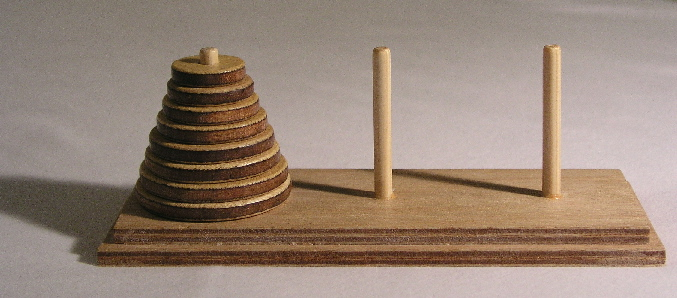
\includegraphics[width=0.8\linewidth]{images/figures/hanoi}
\end{center}
\begin{quote}
``Die Türme von Hanoi''\footnote{Beschreibung und Bild von Wikipedia.} ist ein Geduldspiel. Das Spiel besteht aus drei gleich grossen Stäben A, B und C, auf die mehrere gelochte Scheiben gelegt werden, alle verschieden gross. Zu Beginn liegen alle Scheiben auf Stab A, der Grösse nach geordnet, mit der grössten Scheibe unten und der kleinsten oben. Ziel des Spiels ist es, den kompletten Scheiben-Stapel von A nach C zu versetzen.
Bei jedem Zug darf die oberste Scheibe eines beliebigen Stabes auf einen der beiden anderen Stäbe gelegt werden, vorausgesetzt, dort liegt nicht schon eine kleinere Scheibe. Folglich sind zu jedem Zeitpunkt des Spieles die Scheiben auf jedem Feld der Grösse nach geordnet.
\end{quote}
Wir wollen beweisen, dass ``die Türme von Hanoi'' mit beliebig vielen Scheiben erfolgreich gespielt werden können.
\begin{proof} Wir benutzen ein Induktionsargument ($n$ sei die Anzahl Scheiben):
\begin{itemize}
\item \textbf{Verankerung $n=0$:} Dieser Fall ist trivial, da es keine Scheiben zu bewegen gibt.
\item \textbf{Induktionsschritt $n\to n+1$:} Wir betrachten das Spiel mit $n+1$ Scheiben. Nach Induktionsvoraussetzung gibt es eine Lösungsstrategie für das Spiel mit nur $n$ Scheiben. Diese Strategie können wir offensichtlich dazu verwenden, um alle bis auf die grösste Scheibe auf den Stab B zu verschieben. Nun können wir die grösste Scheibe auf den Stab $C$ verschieben, um anschliessend nochmal die Strategie für das Spiel mit $n$ Scheiben anzuwenden und alle kleineren Scheiben auf den Stab C zu bewegen. Das Spiel ist somit auch für $n+1$ Scheiben lösbar. \qedhere
\end{itemize}
\end{proof}
\begin{rk}
Der Beweis, dass die Türme von Hanoi für beliebige $n$ gelöst werden können, ist mehr als nur eine Argumentationskette, die dazu geeignet ist jemanden davon zu überzeugen, dass es tatsächlich \textit{irgendwie möglich sein muss} das Spiel zu gewinnen. Es steckt viel mehr in diesem Beweis; der Beweis gibt einen konkreten Algorithmus (rekursiv) vor, wie das Spiel erfolgreich gespielt werden kann. Wir betrachten eine Implementierung dieser Lösungsstrategie in Java.


\lstset{language=Java}
\begin{framed}
\begin{lstlisting}
// x-viele Scheiben von A nach B verschieben:
// Falls x=0, dann ist nichts zu tun.
// Sonst, zuerst die oberen (x-1) Scheiben von A nach C
// verschieben,
// dann die groesste Scheibe von A nach B verschieben
// und schliesslich alle anderen Scheiben von C nach B
// verschieben
public class HanoiSolver{

    public String solve(int size){
        return AC(size);
    }

    private String AB(int x){
        if (x==0) return "";
        return AC(x-1)+" AB "+CB(x-1);
    }

    private String AC(int x){
            if (x==0) return "";
            return AB(x-1)+" AC "+BC(x-1);
    }

    private String BC(int x){
            if (x==0) return "";
            return BA(x-1)+" BC "+AC(x-1);
    }

    private String BA(int x){
            if (x==0) return "";
            return BC(x-1)+" BA "+CA(x-1);
    }

    private String CB(int x){
            if (x==0) return "";
            return CA(x-1)+" CB "+AB(x-1);
    }

    private String CA(int x){
            if (x==0) return "";
            return CB(x-1)+" CA "+BA(x-1);
    }
}
\end{lstlisting}
\end{framed}
und die kurze Fassung:
\begin{framed}
\begin{lstlisting}
public class HanoiSolverCompact{

    public String solve(int size){
        return hanoi("A","C","B",size);
    }

    private String hanoi(String x,String y,String z,int n){
        if(n==0) return "";
        return hanoi(x,z,y,n-1)+" "+x+y+hanoi(z,y,x,n-1);
    }
}
\end{lstlisting}
\end{framed}

%\begin{lstlisting}
%let rec AB x =
%    if x=0 then []
%    else (CB (x-1))@(('A','B')::(AC (x-1)))
%
%and AC x =
%    if x=0 then []
%    else (BC (x-1))@(('A','C')::(AB (x-1)))
%
%and BC x =
%    if x=0 then []
%    else (AC (x-1))@(('B','C')::(BA (x-1)))
%
%and BA x =
%    if x=0 then []
%    else (CA (x-1))@(('B','A')::(BC (x-1)))
%
%and CB x =
%    if x=0 then []
%    else (AB (x-1))@(('C','B')::(CA (x-1)))
%
%and CA x =
%    if x=0 then []
%    else (BA (x-1))@(('C','A')::(CB (x-1)))
%
%\end{lstlisting}
\end{rk}
\end{bsp}


\begin{bsp}\label{bsp:plättli}
Ist es immer möglich ein ``gelochtes $n\times n$-Quadrat''
\begin{center}
\begin{tabular}{ | c | c | c | c | c  | c | c | c | }
\hline
&&&&&&&\\
\hline
&&&&&&&\\
\hline
&&&&&&&\\
\hline
&&&&&&&\\
\hline
&&&&&&\cellcolor{black}&\\
\hline
&&&&&&&\\
\hline
&&&&&&&\\
\hline
&&&&&&&\\
\hline
\end{tabular}
\end{center}

mit Flächen von der Form
\begin{tabular}{ c c }
&\cellcolor{black}\\
\cellcolor{black}&\cellcolor{black}
\end{tabular}
``passgenau'' zu überdecken? Ja, wenn $n$ eine Zweierpotenz ist. Wir können diese Behauptung durch Induktion wie folgt beweisen:  Wir nehmen an, dass das ``gelochte Quadrat'' eine Seitenlänge von $2^n$ hat.
\begin{itemize}
\item Verankerung ($n=0$): Wenn $n=0$, dann besteht das gelochte Quadrat nur aus einem Loch. Wir können das Quadrat (ohne etwas zu tun) überdecken.
\item Hat das Quadrat die Seitenlänge $2^{n+1}$, dann zerlegen wir es in vier gleich grosse Quadranten, die alle die Seitenlänge $2^n$ haben. Wir platzieren eine der Flächen wie unten angedeutet (rot).
\begin{center}
\begin{tabular}{ | c | c | c | c !{\color{red}\vrule} c  | c | c | c | }
\hline
&&&&&&&\\
\hline
&&&&&&&\\
\hline
&&&&&&&\\
\hline
&&&\cellcolor{red}&\cellcolor{red}&&&\\
\arrayrulecolor{red}\hline
\arrayrulecolor{black}&&&\cellcolor{red}&&&&\\
\hline
&&&&&&\cellcolor{black}&\\
\hline
&&&&&&&\\
\hline
&&&&&&&\\
\hline
\end{tabular}
\end{center}
Nun sind alle Quadranten ein ``gelochtes Quadrat'' der Seitenlänge $2^n$. Wir können also nach Induktionsvoraussetzung alle Quadranten passgenau belegen.
\end{itemize}
\end{bsp}

\begin{ueb}
Implementieren Sie (ausgehend vom Beispiel~\ref{bsp:plättli}) in einer Programmiersprache Ihrer Wahl, einen Algorithmus zur Überdeckung von ``gelochten Quadraten'', die eine Zweierpotenz als Seitenlänge haben.
\end{ueb}

\section{Rekursive Definitionen}

%\begin{df}
%Eine Menge $X\subseteq \N$ bezeichnen wir als initiales Segment von $\N$ falls mit jeder Nachfolgerzahl\footnote{Eine Nachfolgerzahl ist eine natürliche Zahl die ungleich Null ist} $N(n)=n+1$ welche in $X$ liegt auch deren Vorgänger $n$ ein Element von $X$ ist. Etwas formaler aufgeschrieben ist also $X\subseteq \N$ eine initiale Teilmenge von $\N$ falls die Eigenschaft
%\[
% \forall n\in\N\,\big( n+1\in X\Rightarrow n\in X \big)
%\]
%auf $X$ zutrifft.
%\end{df}

%\begin{bsp}
%Alle Mengen von der Form $\N_{<k}$ mit einer natürlichen Zahl $k$ sind initiale Teilmengen von $\N$. Die %Menge $\N$ selbst ist ebenfalls eine initiale Teilmenge von $\N$.
%\end{bsp}

%\begin{rk}
% Jede nichtleere initiale Teilmenge von $\N$ enthält das Element $0$.
%\end{rk}
%\begin{proof}
 %Sei $M$ folgende Teilmenge von $\N$:
 %\[
 % M:=\{n\in\N\mid \text{es gibt ein initiales Segment }S\text{ mit }0\notin S\text{ und } n\in S\}
% \]
%Wir wollen zeigen, dass $M$ keine Elemente besitzt wir tun dies in dem wir zeigen, dass die Menge $X:=\N\backslash M$ alle natürlichen Zahlen enthält. Wir benützen das Prinzip der vollständigen Induktion. Wäre $0$ nicht in $X$, so wäre $0$ in $M$ dann gäbe es aber ein initiales Segment $S$ mit gleichzeitig $0\in S$ und $0\notin S$, ein Widerspruch. Also ist $0\in X$. sei weiter $n\in X$ dann ist $n\notin M$, es gibt also kein initiales Segment $S$ mit $n\in S$ und $0\notin S$. Gäbe es nun ein initiales Segment $S$ mit $0\notin S$ und $n+1\in S$, dann müsste (da $S$ initial ist) auch $n\in S$ sein woraus aber wieder $n\in M$ folgen würde. Also kann solch ein $S$ nicht existieren und folglich ist $n+1\in X$. Insgesamt habe wir also $X=\N$. Somit kann ein Initiales Segment welches die Null nicht enthält überhaupt keine Elemente enthalten.
%\end{proof}

Rekursive Definitionen bezeichnen die mathematisch einwandfreie Art, ein Objekt durch Bezugnahme (Selbstreferenz) auf das zu definierende Objekt selbst zu definieren.

\begin{bsp}
Ein Palindrom ist ein Wort, das rückwärts und vorwärts gelesen gleich lautet. Beispiele von Palindromen sind $yxy,acaca,arbbra,b,a,\dots$. Obwohl es uns anschaulich klar ist, welche Wörter Palindrome sind und welche nicht, ist unsere Beschreibung keine mathematisch präzise Definition. Dies wird insbesondere dann offensichtlich, wenn wir ein Programm schreiben müssen (ohne ``String-umkehrende'' Operatoren benützen zu dürfen), das von einem gegebenen Wort (String) entscheidet ob dieses ein Palindrom ist oder nicht. Wie können wir also Palindrome definieren (eindeutig beschreiben), ohne auf unsere Vorstellung von rückwärts und vorwärts lesen angewiesen zu sein? Durch Rekursion:\\
Ein Wort $w$ ist ein Palindrom, wenn mindestens eine der beiden folgenden Bedingungen erfüllt ist:
\begin{itemize}
\item Das Wort $w$ besteht aus einem oder gar keinem Buchstaben (Länge von $w$ $<2$).
\item Es gibt einen Buchstaben (Zeichen, Char) $x$ und ein $\underbrace{Palindrom}_{Selbstreferenz}$ $u$ so, dass $w=xux$ gilt.
\end{itemize}
Obwohl diese Definition, durch die in ihr vorhandenen Selbstreferenz, ein wenig ``obskur'' erscheinen mag, können wir sie direkt in ein Computerprogramm übersetzen.\\
In Java:

\lstset{language=Java}
\begin{framed}
\begin{lstlisting}
 boolean palindrome(String w){
     if (w.length() < 2) return true;
     int last = w.length()-1;
     char a = w.charAt(0);
     char b = w.charAt(last);
     if (a == b) return palindrome(w.substring(1, last-1));
     return false;
 }
\end{lstlisting}
\end{framed}
\end{bsp}

\begin{thrm}[Rekursive Definitionen]\label{thrm:rekursive definitionen}
 Ist $M$ eine Menge und $G:M\times\N\rightarrow M$ sowie $c\in M$, dann gibt es eine eindeutig bestimmte Funktion $F:\N\rightarrow M$, welche die Gleichungen (Rekursionsgleichungen)
\begin{align*}
 F(0)&=c\\
F(k+1)&=G(\underbrace{F(k)}_{Selbstbezug},k)
\end{align*}
erfüllt.
\end{thrm}
\begin{proof}[Beweisidee]
Die Behauptung besteht aus einer Eindeutigkeitsaussage und einer Existenzaussage:
\begin{itemize}
\item Die Funktion $F:\N\to M$ ist durch die Rekursionsgleichungen eindeutig bestimmt. Das heisst, dass es keine andere  Funktion gibt, die den Rekursionsgleichungen von $F$ genügt.
\item Es gibt überhaupt eine Funktion, die den Rekursionsgleichungen genügt.
\end{itemize}
Wir beweisen zuerst die Eindeutigkeitsbedingung. Wir nehmen an, dass $F$ und $H$ zwei Funktionen sind, die beide die oben genannten Rekursionsgleichungen erfüllen und zeigen, dass daraus $F=H$ folgt. Es genügt mit Induktion zu zeigen, dass für jede natürliche Zahl $n\in \N$ die Gleichung $F(n)=H(n)$ gilt (weil dann $H=F$ gilt).
\begin{itemize}
\item Verankerung ($n=0$): Aufgrund von
\[
F(0)=c=H(0)
\]
ist die Induktionsverankerung erfüllt.
\item Schritt ($n\to n+1$): Wir nehmen an, dass $F(n)=H(n)$ gilt und müssen $F(n+1)=H(n+1)$ beweisen. Dies folgt sofort aus
\[
F(n+1)=G(F(n),n)\stackrel{IA}{=}G(H(n),n)=H(n+1).
\]
\end{itemize}
Nun kommen wir zur Existenzaussage. Anstelle eines formalen Beweises, wollen wir uns an dieser Stelle bloss anschaulich davon überzeugen, dass eine Funktion $F$ immer existiert. Wir geben einen iterativen Algorithmus (in Pseudocode) an, der die gesuchte Funktion realisiert.
\begin{framed}
\begin{lstlisting}[language=Java]
input(n)
lst=[c] // Eine Liste mit einzigem Eintrag c
for i = 0..(n-1) do
    x = G(lst[i],i)
    lst.add(x) // Den aktuellen Funktionswert zur Liste
               // (aller Funktionswerte) hinzufuegen.
return lst[n]
\end{lstlisting}
\end{framed}\qedhere
\end{proof}
% \begin{rk}
%  Der folgende Beweis ist ziemlich abstrakt, seine Darlegung richtet sich deshalb vor allem an (sehr) interessierte Student(inn)en.
% \end{rk}
% \begin{proof}[Beweis]
%Wir müssen einerseits beweisen, dass bei gegebenem $g:\N\rightarrow M$ und $c\in M$ überhaupt eine Funktion $f:\N\rightarrow M$ existiert welche die Rekursionsgleichungen erfüllt und dann noch zeigen, dass diese eindeutig ist. Wir Beweisen zuerst die \textbf{Eindeutigkeit}. Angenommen, dass es zwei Funktionen $h,f:\N\rightarrow M$ gibt die beide die Rekursionsgleichungen erfüllen, müssen wir zeigen, dass für alle $n\in\N$ die Gleichung $f(n)=h(n)$ gilt. Wir machen einen Induktionsbeweis nach $n$.
%\begin{enumerate}
%\item \textit{Induktionsverankerung:} Es gilt sowohl $f(0)=c$ als auch $h(0)=c$ und somit also $f(0)=h(0)$.
%\item \textit{Induktionsschritt:} Wir können $f(n)=h(n)$ (I.A.) annehmen und müssen $f(n+1)=h(n+1)$ beweisen. Wir betrachten dazu folgende Gleichungen:
%\[
%f(n+1)=g(f(n))\stackrel{I.A.}{=}g(h(n))=h(n+1).
%\]
%\end{enumerate}
%Nun zur \textbf{Existenz} der geforderten Funktion $f$. Seien $g:\N\rightarrow M$ und $c\in M$ gegeben. Für diesen Beweis wollen wir eine Funktion $ h:X\rightarrow M$ als ``gut'' bezeichnen falls $X$ ein initiales Segment von $\N$ ist und für jedes Element $k$ von $X$ die Gleichungen
% \begin{align}\label{glg}
%  h(k)=\begin{cases}
% g(h(n))&\text{ falls }k= n+1 \text{ ein Nachfolger ist}\\
%   c &\text{ falls }k=0.
%  \end{cases}
% \end{align}
% Als nächstes wollen wir mit Induktion zeigen, dass jede natürliche Zahl im Definitionsbereich einer ``guten'' Funktion liegt. Dazu sei $G$ die Menge aller solchen natürlichen Zahlen. Die Zahl $0$ ist in $G$ da die Funktion $h:\{0\}\rightarrow M$ mit $h(0)=c$ eine ``gute'' Funktion ist. Wir nehmen nun an $k$ sei in $G$ und müssen zeigen, dass dann auch $ k+1 \in G$ ist. Da $k$ ein Element von $G$ ist, gibt es also ein initiales Segment $X$ von $\N$ mit $k\in X$ und eine ``gute'' Funktion $h:X\rightarrow M$. Wir erweitern nun folgendermassen $h$ zu einer neuen Funktion $\tilde{h}:X\cup\{ k+1 \}\rightarrow M$:
% \begin{align*}
%  \tilde{h}(n)=\begin{cases}
%                h(n)&\text{ falls }n\in X\\
% 	       g(h(k))&\text{ falls }n= k+1 .
%               \end{cases}
% \end{align*}
% Sei nun $n\in X$ beliebig, dann gilt
% \begin{enumerate}
% \item \textit{Fall} $n\neq 0$: Dann ist $n=m+1$ für ein $m\in X$ und somit $\tilde{h}(n)=h(n)=g(h(m))=g(\tilde{h}(m))$.
%  \item \textit{Fall} $n=0$: Dann ist $ \tilde{h}(n)=\tilde{h}(0)=h(0)=c$.
% \end{enumerate}
% Also erfüllt $\tilde{h}$ die Gleichungen (\ref{glg}) für alle Elemente von $X$. Für die natürliche Zahl $ k+1 $ werden die Gleichungen per Definition erfüllt und da $X\cup\{ k+1 \}$ ein initiales Segment von $\N$ ist folgt, dass $ k+1 \in G$  ist. Also ist mit jedem $k$ auch $ k+1 $ im Definitionsbereich einer ``guten'' Funktion. Mit dem Prinzip der vollständigen Induktion können wir also schliessen, dass alle natürlichen Zahlen diese Eigenschaft haben.
%
%Unser nächster Schritt besteht darin, zu zeigen, dass je zwei ``gute'' Funktionen immer kompatibel\footnote{ Zwei Funktionen $f_1,f_2$ heissen kompatibel, falls für alle $x\in dom(f_1)\cap dom(f_2)$ die Gleichung $f_1(x)=f_2(x)$ erfüllt ist. Dies ist genau dann der Fall wenn $f_1\cup f_2$ eine Funktion ist.} sind. Seien also $f_1,f_2$ gute Funktionen mit $f_1:X_1\rightarrow M$ und $f_2:X_2\rightarrow M$. Wir wollen zeigen, dass für jedes $n\in\N$ gilt, dass entweder $n\notin X_1\cap X_2$ oder $f_1(n)=f_2(n)$ gilt. Wir wenden dafür noch einmal das Prinzip der vollständigen Induktion auf $n$ an.
%\begin{enumerate}
%\item \textit{Induktionsverankerung:} Falls $0\in X_1\cap X_2$ gilt, dann folgt aus der Tatsache, dass $f_1,f_2$ gut sind, die Gleichung $f_1(0)=c=f_2(0)$.
%\item \textit{Induktionsschritt:} Es sei $n+1\in X_1\cap X_2$ (sonst gibt es nichts zu zeigen). Weil $X_1$ und $X_2$ initiale Teilmengen von $\N$ sind gilt $n\in X_1\cap X_2$. Aus der Induktionsannahme folgt also $f_1(n)=f_2(n)$, und somit
%\[
%f_1(n+1)=g(f_1(n))\stackrel{I.A.}{=}g(f_2(n))=f_2(n+1)
%\]
%\end{enumerate}
%Nun definieren wir
%\[
%f:=\bigcup_{h\text{ ist gut}}h
%\]
%Weil gute Funktionen paarweise kompatibel sind erhalten wir, dass $f$ eine Funktion ist und weil jede natürliche Zahl im Definitionsbereich einer guten Funktion liegt, dass
%\[
%f:\N\rightarrow M
%\]
%gilt. Wir müssen noch zeigen, dass $f$ den Rekursionsgleichungen genügt. Es sei $h:X\rightarrow M$ eine guten Funktion mit $0\in X$ (eine solche gibt es da jedes $n\in\N$ im Definitionsbereich einer guten Funktion liegt). Es gilt $f(0)=h(0)=c$. Sei nun $n\in\N$ beliebig und $h:X\rightarrow M$ eine gute Funktion mit $n+1\in X$. Weil $X$ eine initiale Teilmenge von $\N$ ist gilt, dass $n$ in $X$ liegt und somit
%\[
%f(n+1)=h(n+1)=g(h(n))=g(f(n)).
%\]
%\end{proof}

\begin{bsp}\label{bsp:rekursive operationen}
Die üblichen arithmetischen Grundoperationen können alle relativ kompakt als rekursive Definitionen geschrieben werden:
\begin{itemize}
\item Die Addition von natürlichen Zahlen:
\begin{align*}
x+0&=x\\
x+(n+1)&=(x+n)+1
\end{align*}
\item Die Multiplikation von natürlichen Zahlen:
\begin{align*}
x\cdot 0 &= 0\\
x\cdot(n+1)&=(x\cdot n)+x
\end{align*}
\item Die Exponentiation von natürlichen Zahlen:
\begin{align*}
x^0&=1\\
x^{n+1}&=x\cdot x^{n}
\end{align*}
\item Die Fakultätsfunktion:
\begin{align*}
0!&=1\\
(n+1)!&=n!\cdot(n+1)
\end{align*}
\item Endliche Summen:
\begin{align*}
\sum_{i=1}^{0}a_i&=0\\
\sum_{i=1}^{n+1}a_{i}&=(\sum_{i=0}^na_i)+a_{n+1}
\end{align*}
\item Endliche Produkte:
\begin{align*}
\prod_{i=1}^{0}a_i&=1\\
\prod_{i=1}^{n+1}a_i&= (\prod_{i=1}^na_i)\cdot a_{n+1}
\end{align*}
\end{itemize}
\end{bsp}
Die üblichen Rechenregeln für natürliche Zahlen lassen sich aufgrund dieser rekursiven Definitionen mit Induktion (und genügend Geduld) beweisen. Wir beschränken uns beispielhaft auf den Beweis von Satz~\ref{satz:partialsummen}.

\begin{ueb}
	Implementieren Sie alle Funktionen von Beispiel \ref{bsp:rekursive operationen} in der Programmiersprache Ihrer Wahl (natürlich ohne Verwendung der vorimplementierten Grundoperationen). Halten Sie sich so präzise wie möglich an die mathematische Definition.
\end{ueb}
\begin{lsg}
	\ifthenelse{\boolean{ml}}{
		Vgl. OLAT ``rekursive Operationen''}{
		Elektronisch zu lösen.}
\end{lsg}

\begin{satz}\label{satz:additionsregeln}
Für alle natürlichen Zahlen $n,m,k$ gelten folgende Rechenregeln für deren Addition:
\begin{enumerate}
\item Neutrales Element: $0+n=n$
\item Kommutativität: $n+m=m+n$
\item Assoziativität: $(n+m)+k=n+(m+k)$
\item Kürzbarkeit: $n+k=m+k\Rightarrow n=m$
\end{enumerate}
\end{satz}


\begin{rk}
Wegen der Assoziativität der Addition, können wir Klammern in endlichen Summen von natürlichen Zahlen weglassen.
\end{rk}




\begin{satz}[Rechenregeln für die Multiplikation]\label{satz:multiplikationsregeln}
Für alle $n,m,k\in\N$ gelten folgende Identitäten\footnote{Wir vereinbaren hier, dass die Multiplikation ``stärker bindet'' als die Addition. Ein Ausdruck von der Form $nm+k$ wird also als $(nm)+k$ interpretiert.}:
\begin{enumerate}
\item \textit{Absorbtion:} $0\cdot n=0$
\item \textit{Neutrales Element:} $1\cdot n=n$
\item \textit{Kommutativität:} $n\cdot m=m\cdot n$
 \item \textit{Assoziativität:} $n\cdot(m\cdot k)=(n\cdot m)\cdot k$
\item \textit{Distributivität:} $n\cdot(m+k)=nm+nk$
\end{enumerate}
\end{satz}
\begin{ueb}
	Nachdem wir die Addition und die Multiplikation rekursiv definiert haben, lassen sich dies in den Sätzen \ref{satz:additionsregeln} und \ref{satz:multiplikationsregeln} geäusserten Tatsachen durch Induktion beweisen. Die einzelnen Beweise sind nicht sonderlich spannend aber eine gute Übung.
\end{ueb}


\begin{satz}[Rechenregeln für Partialsummen]\label{satz:partialsummen}
 Sind $(a_i)_{i\in\N}$ und $(a_i)_{i\in\N}$ beliebige Folgen und ist $c\in\N$, dann gilt für jedes $n\in\N$:
\[
 \sum_{i=1}^n(ca_i+cb_i)=c\big(\sum_{i=1}^na_i+\sum_{i=1}^nb_i\big)
\]
\end{satz}
\begin{proof}
 Induktion nach $n$.
 \begin{itemize}
 \item Verankerung ($n=0$): Die Verankerung gilt aufgrund von
 \begin{align*}
\sum_{i=1}^0(ca_i+cb_i)=0=c(0+0)=c\big(\sum_{i=1}^0a_i+\sum_{i=1}^0b_i\big).
 \end{align*}
 \item Schritt ($n\to n+1$):
 \begin{align*}
\sum_{i=1}^{n+1}(ca_i+cb_i)&=\big(\sum_{i=1}^n(ca_i+cb_i)\big)+(ca_{n+1}+cb_{n+1})\\
&=\big(\sum_{i=1}^n(ca_i+cb_i)\big)+c(a_{n+1}+b_{n+1})\\
&\stackrel{IA}{=}c\big(\sum_{i=1}^na_i+\sum_{i=1}^nb_i\big)+c(a_{n+1}+b_{n+1})\\
&=c\big( \sum_{i=1}^na_i+\sum_{i=1}^nb_i+a_{n+1}+b_{n+1} \big)\\
&=c\big( \sum_{i=1}^na_i+a_{n+1}+\sum_{i=1}^nb_i+b_{n+1} \big)\\
&=c\big( \sum_{i=1}^{n+1}a_i+\sum_{i=1}^{n+1}b_i\big)\qedhere
 \end{align*}
 \end{itemize}
\end{proof}



\chapter{Elementare Zahlentheorie}




\section*{Lernziele}
Sie kennen die
\begin{itemize}
\item Grundlagen der Teilbarkeitslehre.
\item den Begriff der Primzahl.
\item das kgV und den ggT und wie diese mithilfe des  euklidischen Algorithmus berechnet werden.
\item das Lemma von Bézout.
\item den chinesischen Restsatz.
\item den kleinen Fermatschen Satz.
\end{itemize}
Sie verstehen
\begin{itemize}
\item wieso und wie ganze Zahlen in ihre Primfaktoren zerlegt werden können.
\item die modulare Arithmetik.
\item den Zusammenhang vom chinesischen Restsatz und der Lösbarkeit von simultanen Kongruenzen.
\end{itemize}
Sie sind in der Lage
\begin{itemize}
\item die Stellenwertsysteme ineinander umzurechnen.
\item Systeme simultaner Kongruenzen aufzulösen.
\end{itemize}


\section*{Literatur und Links}
\begin{itemize}
\item Euklidischer Algorithmus:\\
\url{http://de.wikipedia.org/wiki/Euklidischer_Algorithmus}\\
\end{itemize}


Analog zu unserem Vorgehen mit den natürlichen Zahlen wollen wir auch die \textit{ganzen Zahlen} informell einführen. Wir definieren
\[
\Z:= \{..,-2,-1,0,1,2,...\}.
\]
Die Motivation die Menge $\N$ zur Menge $\Z$ erweitern zu wollen fusst auf der Tatsache, dass für feste natürliche Zahlen $k,k'$ im Allgemeinen die Gleichung
\[
 k+x=k'
\]
keine Lösung in $\N$ besitzt. Es ist in der Tat so, dass bei der Konstruktion von $\Z$ aus $\N$ (was wir nicht tun werden) die Menge $\Z$ im Prinzip als die Menge aller Lösungen von solchen Gleichungen eingeführt wird.

Wir wollen es als gegeben erachten, dass die Multiplikation und die Addition derart von $\N$ auf $\Z$ fortgesetzt werden können, dass folgende Rechenregeln bestehen:

\begin{rk}[Rechenregeln auf $\Z$]
Für alle $r,s,z\in\Z$ gelten folgende Gleichungen.
\begin{align*}
-1\cdot z&=-z\\
-(-z)&=z\\
-z+z&=0 &\text{ Inverse Elemente bezüglich }+\\
0\cdot z&=0 &\text{ Absorbtion}\\
1\cdot z&=z &\text{ Neutrales Element bezüglich }\cdot\\
0+z&=z &\text{ Neutrales Element bezüglich }+\\
r(sz)&=(rs)z &\text{ Assoziativität von } \cdot\\
r+(s+z)&=(r+s)+z &\text{ Assoziativität von }+\\
rs&=sr &\text{ Kommutativität von }\cdot\\
r+s&=s+r &\text{ Kommutativität von }+\\
r(s+z)&=rs+rz &\text{ Distributivität}\\
rx=ry&\Rightarrow x=y\lor r=0&\text{Kürzbarkeit}
\end{align*}
\end{rk}

\begin{df}
 Wir definieren die \textit{Subtraktion}
\[
 -:\Z\times\Z\rightarrow\Z
\]
durch
\[
 x-y:=x+(-y),
\]
die \textit{Betragsfunktion}
\[
 |\cdot|:\Z\rightarrow\N
\]
durch
\[
 |z|=\begin{cases}
      z&\text{falls } z\in\N\\
      -1\cdot z&\text{sonst}
     \end{cases}
\]
und die Relation $\leq$ durch
\[
x\leq y:\Leftrightarrow\,\exists n\in\N\,(x+n=y).
\]
\end{df}



\section{Teilbarkeit und Euklidischer Algorithmus}
\begin{df}
 Sind $x,y\in\mathbb{Z}$ ganze Zahlen, so sagen wir, dass $x$ \textit{ein Teiler von} $y$ ist, falls es ein $k\in\mathbb{Z}$ gibt mit $xk=y$. Wir schreiben in diesem Fall $x|y$. Es gilt also
\[
 x|y:\Leftrightarrow \exists k\in\Z(y=xk).
\]
Mit $T(y)$ bezeichnen wir die Menge aller natürlichen Zahlen, welche Teiler von $y$ sind, also $T(y)=\{x\in\N\mid x|y\}$.
\end{df}
\begin{bsp}~
 \begin{enumerate}
  \item Die Zahl $1$ ist ein Teiler jeder ganzen Zahl $z$, da $1\cdot z=z$.
\item $T(0)=\N$.
 \end{enumerate}

\end{bsp}
\begin{rk}
 Die Teilbarkeitsrelation ist reflexiv und transitiv auf der Menge $\Z$, auf der Menge $\N$ ist die Teilbarkeitsrelation sogar eine Halbordnung (wieso nicht auf der Menge $\Z$?).
\end{rk}
\begin{proof}
Wir zeigen, dass die Teilbarkeitsrelation reflexiv, transitiv und für natürliche Zahlen auch antisymmetrisch ist.
\begin{itemize}
\item Reflexivität: Dies gilt, da jede ganze Zahl sich selbst teilt.
\item Transitivität: Seien $x,y,z$ ganze Zahlen. Aus $x|y$ und $y|z$ folgt, dass es ganze Zahlen $k_1,k_2$ gibt mit $x\cdot k_1=y$ und $y\cdot k_2=z$. Es folgt
\[
x\cdot(k_1\cdot k_2)=(x\cdot k_1)\cdot k_2=y\cdot k_2=z.
\]
 Somit existiert eine ganze Zahl $k$ (nämlich $k=k_1\cdot k_2$) mit $k\cdot x=z$, also gilt $x|z$ wie gewünscht.\qedhere
\item Antisymmetrie auf $\N$: Wir müssen zeigen, dass für natürliche Zahlen $x$ und $y$ aus $x|y$ und $y|x$ folgt, dass $x=y$ gilt. Es gelte also $xk=y$ und $x=yr$ für ganze Zahlen $k,r$. Es folgt
\[
x=yr=(xk)r=x(kr)
\]
und $kr=1$. Daraus ergeben sich zwei mögliche Fälle; $k=r=1$ oder $k=r=-1$. Im Fall $k=r=-1$ folgt $x=-y$, was im Widerspruch dazu steht, dass $x$ und $y$ natürliche Zahlen sind. Es bleibt also nur der Fall $k=r=1$ und somit, wie gewünscht, $x=y$.
\end{itemize}
\end{proof}

\begin{bsp}
Das Hasse-Diagramm der Teilbarkeitsrelation auf der Menge $T(30)$:
\begin{center}
\begin{tikzpicture}[scale=0.8]
  \node (1) at (0,0) {$1$};
  \node (2) at (2,2) {$2$};
  \node (3) at (-2,2) {$3$};
  \node (5) at (0,2) {$5$};
  \node (15) at (-2,4) {$15$};
  \node (6) at (0,4) {$6$};
  \node (10) at (2,4) {$10$};
  \node (30) at (0,6) {$30$};
  \draw (1) -- (3) -- (15) -- (30) -- (10) -- (2)--(1)--(5)--(15)--(3)--(6)--(2);
  \draw (5) -- (10);
  \draw (6) -- (30);
\end{tikzpicture}
\end{center}
Das Hasse-Diagramm der Teilbarkeitsrelation auf der Menge $T(90)$:
\begin{center}
\begin{tikzpicture}[scale=0.8]
  \node (1) at (0,0) {$1$};
  \node (2) at (2,2) {$2$};
  \node (3) at (-2,2) {$3$};
  \node (5) at (0,2) {$5$};
  \node (15) at (-2,4) {$15$};
  \node (6) at (0,4) {$6$};
  \node (10) at (2,4) {$10$};
  \node (30) at (0,6) {$30$};
  \node (45) at (-4,6) {$45$};
  \node (18) at (-2,6) {$18$};
  \node (9) at (-4,4) {$9$};
  \node (90) at (-2,8) {$90$};
  \draw (1) -- (3) -- (15) -- (30) -- (10) -- (2)--(1)--(5)--(15)--(3)--(6)--(2);
  \draw (5) -- (10);
  \draw (6) -- (18)--(9)--(3)--(15)--(45)--(90)--(30);
  \draw (6) -- (30);
  \draw (9) -- (45);
  \draw (18) -- (90);
\end{tikzpicture}
\end{center}
\end{bsp}

\begin{rk}\label{Zeinheiten}
Sind $x,y\in\Z$ und gilt $x\cdot y=1$ so gilt $|x|=|y|=1$.
\end{rk}


\begin{satz}[Teilen mit Rest]
 Sind $n,m\in\N\backslash\{0\}$, dann gibt es eindeutig bestimmte Zahlen $k,r\in\N$, so dass Folgendes gilt:
\begin{enumerate}
\item $m=kn+r$
 \item $r<n$
\end{enumerate}
Wir sagen in diesem Zusammenhang, dass die Zahl $r$ den \textit{Rest} von der (ganzzahligen) Division von $m$ durch $n$ ist.
\end{satz}
\begin{proof}
 Seien $n,m\in\N\backslash\{0\}$ beliebig. Die Menge
\[
 M:=\{k\in\N\mid kn\leq m\}
\]
ist endlich (da $n\geq 1$), somit gibt es ein maximales Element $k_0\in M$. Wir definieren $r:=m-k_0n$. Da $k_0\in M$ gilt, ist $r\in\N$. Es gilt
\[
 k_0n+r=k_0n+(m-k_0n)=m.
\]
Falls $r\geq n$ wäre, dann würde
\[
 m-(k_0+1)n=m-(k_0n+n)=r-n\geq 0
\]
und somit $k_0+1\in M$ gelten, was im Widerspruch zur Maximalität von $k_0$ in $M$ steht. Wir müssen nun noch die Eindeutigkeit zeigen. Es genügt zu zeigen, dass für $r,r'<n$
\[
 (kn+r=k'n+r')\Rightarrow (k=k')
\]
gilt. Wir machen einen Beweis durch Widerspruch und nehmen also $k\neq k'$ an. Aus Symmetriegründen können wir $k<k'$ und somit $k'=k+p$ mit $p>0$ annehmen. Es gilt also
\begin{align*}
 kn+r=k'n+r'=(k+p)n+r'=kn+pn+r'
\end{align*}
und somit
\[
 r=pn+r'\geq n,
\]
ein Widerspruch.
\end{proof}

\begin{ueb}
	Schreiben Sie in der Programmiersprache Ihrer Wahl eine Funktion, die zwei positive ganze Zahlen mit Rest teilt (natürlich ohne die Verwendung des Modulo Operators).
\end{ueb}
\begin{lsg}
	\ifthenelse{\boolean{ml}}{
        Vgl. Code in der Vorlesung.
		}{~
		Elektronisch zu lösen.
	}
\end{lsg}

\begin{df}
Seien $n,m\in\Z$. Wir definieren das \textit{kleinste gemeinsame Vielfache von $n$ und $m$} als
\[
 kgV(n,m):=\min\{k\in\N\mid n|k\wedge m|k\}.
\]
Ist $n\neq0$ oder $ m\neq 0$, dann definieren wir den \textit{grössten gemeinsamen Teiler} von $n$ und $m$ als
\[
 ggT(n,m):=\max\{k\in\N\mid k|n\wedge k|m\}.
\]
\end{df}

\begin{lm}\label{lm:lemmaggT}
 Sind $x,y,z\in\Z$, dann sind folgende Aussagen äquivalent:
\begin{enumerate}
\item[1.] $ x|y\wedge x|z$
\item[2.] $x|y\wedge x|(y-z) $
\end{enumerate}
\end{lm}
\begin{proof}
 $1.\Rightarrow 2.$: Wenn $x|y\wedge x|z$, dann gibt es ganze Zahlen $k,k'\in\Z$, so dass $y=kx$ und $z=k'x$. Es gilt also $y-z=kx-k'x=(k-k')x$.

$2.\Rightarrow 1.$: Es seien $k,k'\in\Z$, so dass $y=kx$ und $y-z=k'x$. Durch Einsetzen erhält man $ kx-z=k'x $ und somit $z=kx-k'x=x(k-k')$.
\end{proof}

\begin{satz}[Euklidischer Algorithmus]\label{satz:euklid}
 Für $n,m\in\N$ mit $0<n< m$ gilt
\[
 ggT(n,m)=ggT(n,m-n)=ggT(m,m-n).
\]
\end{satz}
\begin{proof}
Aus Lemma~\ref{lm:lemmaggT} folgt für $n,m\in\N$ mit $n<m$
\[
\{k\in\N\mid k|n\wedge k|m\}=\{k\in\N\mid k|n\wedge k|(m-n)\}.
\]
Daraus folgt weiter
\begin{align*}
ggT(n,m)=\max\{k\in\N\mid k|n\wedge k|m\}=\max\{k\in\N\mid k|n\wedge k|(m-n)\}=ggT(n,m-n).
\end{align*}
Die Gleichung
\[
 ggT(n,m)=ggT(m,m-n)
\]
folgt analog aus Lemma~\ref{lm:lemmaggT}.
\end{proof}

\begin{rk}[Euklidischer Algorithmus]
Aus dem eben bewiesenen Satz~\ref{satz:euklid} erhalten wir direkt einen rekursiven Algorithmus zur Berechnung des $ggT$. Beispielhaft geht man dabei wie folgt vor:
\begin{align*}
ggT(45,25)&\stackrel{Satz~\ref{satz:euklid}}{=}ggT(25,20)\\
&\stackrel{Satz~\ref{satz:euklid}}{=}ggT(20,5)\\
&\stackrel{Satz~\ref{satz:euklid}}{=}ggT(5,15)\\
&\stackrel{Satz~\ref{satz:euklid}}{=}ggT(5,10)\\
&\stackrel{Satz~\ref{satz:euklid}}{=}ggT(5,5)=5.
\end{align*}
Dieses Vorgehen lässt sich direkt in Java umsetzen:
\begin{framed}
\begin{lstlisting}[language=Java]
int ggT(int n,int m){
    if(n == m) return n;
    if(n < m) return ggT(n, m - n);
    return ggT(m, n - m);
}
\end{lstlisting}
\end{framed}
Betrachten wir nochmals den Satz~\ref{satz:euklid}, dann sehen wir, dass wir mehrere Schritte zu einem einzigen Schritt zusammenfassen können. Bei $x>y$ wird nämlich, zum Berechnen von $ggT(y,x)$ so oft $y$ von $x$ subtrahiert, bis das Resultat kleiner oder gleich $y$ ist. Man kann all diese Subtraktionen also durch eine einzige Division mit Rest ersetzen.
Die beispielhafte Berechnung von $ggT(45,25)$ können wir nun als $2$ Divisionen mit Rest darstellen:
\begin{align*}
45 &= 1 \cdot 25 + 20\\
25 &= 1 \cdot 20 + \underbrace{5}_{ggT(45,25)}.
\end{align*}
Zusammenfassend stellen wir fest, dass
\[
ggT(y,x)=ggT(y,R(x,y))
\]
mit
\[
R(x,y)=\text{ der Rest der Division von }x\text{ durch }y
\]
gilt. Die Funktion $R(x,y)$ steht in vielen Programmiersprachen als ``modulo Funktion'' zur Verfügung und wird im Quellcode oft durch das Prozentzeichen $\%$ aufgerufen. Dies eröffnet die Möglichkeit den euklidischen Algorithmus kompakter zu notieren:\\

\lstset{language=Java}
\begin{framed}
\begin{lstlisting}
int ggT(int n, int m){
    if(n == 0) return m;
    if(n < m) return ggT(m % n, n);
    return ggT(n % m, m);
}
\end{lstlisting}
\end{framed}
\end{rk}

\begin{ueb}
	Benutzen Sie den euklidischen Algorithmus um $ggT(27,96)$ auszurechnen (notieren Sie die Zwischenresultate).
\end{ueb}
\begin{lsg}
	\ifthenelse{\boolean{ml}}
		{
			\begin{align*}
				ggT(27,96) &= ggT(96 \% 27, 27)\\
				 &= ggT(15, 27) = ggT(27 \%15,15)\\
				 &=ggT(12,15)=ggT(15 \%12,12)\\
				 &=ggT(3,12)=ggT(12\%3,3)\\
				 &=ggT(0,3)=3
			\end{align*}
		}
		{~
			\answerspace{6cm}
		}
\end{lsg}
\begin{df}
 Zwei ganze Zahlen $x,y$ heissen \textit{teilerfremd}, wenn $ggT(x,y)=1$ gilt.
\end{df}

%\begin{ern}
%In den übungen haben Sie bewiesen, dass man das Prinzip der vollständigen Induktion dahingehend verallgemeinern kann, dass man in der Induktionsannahme auf alle ``Vorgängerfälle'' Bezug nehmen darf. Formal haben Sie gezeigt, für jede Menge $X\subseteq\N$ mit der Eigenschaft
%\[
%\forall n\in\N\big(\forall m<n\,(m\in X\Rightarrow n\in X)\big),
%\]
%$X=\N$ gilt. Dieses Verfahren werden wir im folgenden Beweis anwenden.
%\end{ern}

\begin{thrm}[Lemma von Bézout]\label{hauptideal}
Sind $x,y\in\Z$ mit $x,y\neq 0$, dann gibt es ganze Zahlen $a,b$ so dass
\[
 ggT(x,y)=ax+by
\]
gilt. Die Zahlen $a$ und $b$ werden Bézout Koeffizienten genannt.
\end{thrm}
\begin{proof}
	Wir können ohne Einschränkung der Allgemeinheit $x,y\geq 1$ annehmen und die Behauptung
	\begin{align*}
		\forall x,y\geq 1\;\exists a,b\in\Z\;(ggT(x,y)=ax+by).
	\end{align*}
	beweisen. Wir führen den Beweis durch Widerspruch. Es gebe also natürliche Zahlen $x,y\geq 1$ mit
	\begin{align*}
		\varphi(x,y):\Leftrightarrow \forall a,b\in\Z\;(ax+by\neq ggT(x,y)).
	\end{align*}
	Insbesondere existieren folgende kleinste natürliche Zahlen (Methode des kleinsten Verbrechers):
	\begin{align*}
		x_0&=\min \{n\geq 1 \mid \exists k\geq 1\;\varphi(n,k)\} = \min\{n\geq 1 \mid \exists k\geq 1\,\forall a,b\in\Z\;(an+bk\neq ggT(n,k))\}\\
		y_0&=\min \{n\geq 1 \mid \varphi(x_0,n)\}=\min\{n\geq 1 \mid \forall a,b\in\Z\;(ax_0+bn\neq ggT(x_0,n))\}
	\end{align*}
	Es gilt offensichtlich $x_0\neq y_0$ und $\varphi(x,y)\Leftrightarrow\varphi(y,x)$. Wir können daher ohne Einschränkung $x_0<y_0$ annehmen. Weil $1\leq y_0-x_0<y_0$ gilt, gibt es ganze Zahlen $a,b\in\Z$ mit $ax_0+b(y_0-x_0) = ggT(x_0,y_0-x_0)$. Mit dem Euklidischen Algorithmus folgt daraus der gesuchte Widerspruch (zur Wahl von $x_0$ und $y_0$):
	\begin{align*}
		(a-b)x_0+by_0 &=ax_0-bx_0+by_0\\
				      &=ax_0+b(y_0-x_0)\\
					  &= ggT(x_0,y_0-x_0)\\
					  &=ggT(x_0,y_0)
	\end{align*}



%Wir beweisen das Theorem exemplarisch für den Fall, dass $ggT(m,n)=1$ gilt. Ohne Einschränkung sei $m>n$. Sind $x,y$ beliebige ganze Zahlen, dann bezeichnen wir
%\begin{align*}
%R(x,y):=\begin{cases}
%\text{ Der Rest von der ganzzahligen Division von $x$ durch $y$}&\text{falls }x,y>0\\
%0&\text{sonst.}
%\end{cases}
%\end{align*}
%Wir definieren rekursiv eine absteigende Folge $(r_i)_{i\in\N}$ von natürlichen Zahlen wie folgt:
%\begin{align*}
%r_i=\begin{cases}
%m&\text{falls }i=0\\
%n&\text{falls }i=1\\
%R(r_{i-2},r_{i-1})&\text{sonst.}
%\end{cases}
%\end{align*}
%Da es keine echt absteigende Folge von natürlichen Zahlen gibt, muss die Folge der $(r_i)_{i\in\N}$ stationär werden. Es folgt also aus der Definition der Folge $(r_i)_{i\in\N}$, dass es ein $p\in\N$ gibt, so dass $r_{p}\neq0$ und für alle $p`>p$ gilt $r_{p`}=0$. Es sei $(\lambda_i)_{i\in\N}$ die durch $(r_i)_{i\in\N}$ eindeutig bestimmte Folge natürlicher Zahlen mit der Eigenschaft (*):
%\begin{align*}
%r_0&=\lambda_0\cdot r_1+r_2\\
%r_1&=\lambda_1\cdot r_2+r_3\\
%&\vdots\\
%r_{p-2}&=\lambda_{p-2}\cdot r_{p-1}+r_{p}
%\end{align*}
%\textbf{Behauptung}: $r_p=1$\\
%\textbf{Beweis}: Wir zeigen, dass $r_p$ ein Teiler von allen $r_i$ mit $i\leq p$ ist. Weil $r_0=m,r_1=n$ teilerfremd sind, gilt dann $r_p=1$. Wir beweisen mit (der allgemeinen Version von) Induktion für alle $k\in\N$, dass entweder $r_p|r_{p-k}$ oder $k>p$ gilt.
%Falls $k>p$ ist, dann sind wir fertig. Wir können also ohne Einschränkung der Allgemeinheit annehmen, dass $k\leq p$ gilt. Nach Induktionsannahme ist nun $r_p$ ein Teiler von $r_{p-(k-1)}$ und von $r_{p-(k-2)}$, es gibt also ganze Zahlen $x,y$ mit $x\cdot r_p=r_{p-(k-1)}$ und $y\cdot r_p=r_{p-(k-2)}$. Insgesamt haben wir dann
%\begin{align*}
%r_{p-k}=\lambda_{p-k}\cdot r_{p-k+1}+r_{p-k+2}=\lambda xr_{p}+yr_{p}=r_{p}(\lambda x+y)
%\end{align*}
%und somit wie gewünscht, dass $r_p$ ein Teiler von $r_{p-k}$ ist.\\
%Wir können nun das Gleichungssystem $(*)$ als
%\begin{align*}
%r_0&=\lambda_0\cdot r_1+r_2\\
%r_1&=\lambda_1\cdot r_2+r_3\\
%&\vdots\\
%r_{p-2}&=\lambda_{p-2}\cdot r_{p-1}+1
%\end{align*}
%schreiben. Dies ist jedoch mit
%\begin{align*}
%1&=r_{p-2}-\lambda_{p-2}r_{p-1}\\
%r_{p-1}&=r_{p-3}-\lambda_{p-3}r_{p-2}\\
%&\vdots\\
%r_{p-i}&=r_{p-i-2}-\lambda_{p-i-2}r_{p-i-1}\\
%&\vdots\\
%\underbrace{r_{p-p+2}}_{r_2}&=\underbrace{r_{p-p}}_{m}-\lambda_{0}\underbrace{r_{p-p+1}}_{n}
%\end{align*}
%äquivalent. Indem wir nun sukzessiv (von unten beginnend) in jeder Zeile des Gleichungssystems die $r_i$ auf der rechten Seite durch eine Summe von Vielfachen von $n$ und $m$ ersetzen, erhalten wir zuoberst im Gleichungssystem für geeignete $s,\delta_i,\gamma_i$ eine Gleichung von der gewünschten Gestalt
%\[
%1=\sum_{i=1}^{s}\delta_in-\gamma_im=\sum_{i=1}^{s}\delta_in-\sum_{i=1}^{s}\gamma_im=n\sum_{i=1}^{s}\delta_i-m\sum_{i=1}^{s}\gamma_i.\qedhere
%\]
\end{proof}

\begin{ueb}
	Zeigen Sie, dass Bézout Koeffizienten nicht eindeutig sind.
	\begin{lsg}
		Es sei en $a$ und $b$ Bézout Koeffizienten von $x$ und $y$. Es gilt:
		\begin{align*}
			ggT(a,b) = ax+by = ax+by+xy-xy=ax+xy+by-xy=(a+y)x+(b-x)y
		\end{align*}
	\end{lsg}
\end{ueb}


\begin{bsp}
 Wir wollen ganze Zahlen $a$ und $b$ finden, die die Gleichung
 \[
 a\cdot 504+b\cdot 29=ggT(504,29)=1
 \]
 erfüllen.
\begin{itemize}
 \item Schritt 1: Sukzessives Teilen mit Rest.
\begin{align*}
	504 &= 17 \cdot 29 + 11\\
	29 &= 2 \cdot 11 + 7\\
	11 &= 1 \cdot 7 + 4\\
	7 &= 1 \cdot 4 + 3\\
	4 &= 1 \cdot 3 + \underbrace{1}_{ggT(504,29)}.
\end{align*}
 \item Schritt 2: ``Rückwärts einsetzen''.
 \begin{align*}
	1&=4-3\\
	&=(11-7)-(7-4)\\
	&=((504-17\cdot 29)-(29-2\cdot 11))-((29-2\cdot 11)-(11-7))\\
	&=((504-17\cdot 29)-(29-2\cdot (504-17\cdot 29)))\\
	&\phantom{abst}-((29-2\cdot (504-17\cdot 29))-((504-17\cdot 29)-(29-2\cdot 11)))\\
	&=((504-17\cdot 29)-(29-2\cdot (504-17\cdot 29)))
	-((29-2\cdot (504-17\cdot 29))\\
	&\phantom{abst}-((504-17\cdot 29)-(29-2\cdot (504-17\cdot 29)))).
 \end{align*}
	\item Schritt 3: Zusammenfassen (Zählen der Vorkommen von $504$ und $29$).
 \begin{align*}
 	a&=1+2+2+1+2=8\\
 	b&=-17-1-(2\cdot 17)-1-(2\cdot 17)-17-1-(2\cdot 17)=-139
 \end{align*}
\item Test:
 \[
 8\cdot 504-139\cdot 29=1.
 \]
\end{itemize}
\end{bsp}


%\begin{satz}
% Für $n,m\in\N\backslash\{0\}$ gilt
%\[
% kgV(n,m)\cdot ggT(n,m)=nm
%\]
%\end{satz}
%\begin{proof}
% übung
%\end{proof}
%
%\begin{df}
%Wir definieren nun rekursiv in $n$, den $ggT$ nun für beliebige $n$-Tupel $(n>0)$:
%\begin{align*}
%ggT(x_0)&=x_0\\
%ggT(x_0,..,x_n,x_{n+1})&=ggT(ggT(x_1,..,x_n),x_{n+1})
%\end{align*}
%\end{df}
%
%
%\begin{ueb}
%\begin{enumerate}
%\item Berechnen Sie $ggT(125,75)$ mit dem Euklidischen Algorithmus.
%\item Beweisen Sie, dass für alle $n\in\N_{>0}$
%\[
%ggT(x_1,..,x_n)=\max\{k\in\N \mid (k|x_1)\wedge (k|x_2)\wedge..\wedge (k|x_n) \}
%\]
%gilt.
%\item Um $5:45$ Uhr fahren an einer Bushaltestelle die Busse der Linie $1,2$ und $3$ gemeinsam ab. Die Linie $1$ fährt von da an alle $6$ Minuten, die Linie $2$ alle $14$ Minuten und die Linie $3$ alle $11$ Minuten. Wie oft fahren die Busse, bis zum Betriebsschluss um $23:00$ Uhr, aller Linien gemeinsam ab?
% \end{enumerate}
%\end{ueb}

\begin{ueb}
	Finden Sie ganze Zahlen $a$ und $b$, die folgende Gleichung erfüllen:
	\[
		a\cdot 3215 + b\cdot 123 = 1.
	\]
	\begin{lsg}
		\ifthenelse{\boolean{ml}}
			{
				Sukzessives Teilen mit Rest ergibt:
				\begin{align*}
					3215 &= 26 \cdot 123 + 17\\
					123 &= 7 \cdot 17 + 4\\
					17 &= 4 \cdot 4 + 1.
				\end{align*}
				Wir erhalten somit:
				\begin{align*}
					1 &=  17-4\cdot 4\\
					&= (3215-26\cdot 123)-4\cdot (123-7\cdot 17)\\
					&= (3215-26\cdot 123)-4\cdot (123-7\cdot (3215-26\cdot 123))\\
					&= 29\cdot 3215-758\cdot 123.
				\end{align*}
				Also gilt $a=29$ und $b=-758$.
			}
			{~\answerspace{12cm}}
	\end{lsg}
\end{ueb}
\section{Primzahlen}

Primzahlen sind natürliche Zahlen, die genau zwei natürliche Zahlen als Teiler haben. Eine dazu äquivalente Formulierung ist, dass eine Primzahl eine von $1$ verschiedene natürliche Zahl ist, die (in $\N$) nur durch sich selbst und durch $1$ teilbar ist. Die ersten $25$ Primzahlen sind:
\[
2, 3, 5, 7, 11, 13, 17, 19, 23, 29, 31, 37, 41, 43, 47, 53, 59, 61, 67, 71, 73, 79, 83, 89, 97
\]

\begin{df}
Eine natürliche Zahl $p\in\N$ ist eine \textit{Primzahl}, wenn $|T(p)|=2$ gilt. Die Menge aller Primzahlen bezeichnen wir mit $\mathbb{P}$.
\end{df}

\begin{rk}
Ist $p$ eine Primzahl, dann gilt $T(p)=\{1,p\}$.
\end{rk}
\begin{proof}
Für jede Zahl $n\in\N$ gilt offensichtlich $n\in T(n)$ und $1\in T(n)$. Bei Primzahlen kommt dazu, dass (wegen $|T(n)|=2$) keine weiteren Teiler existieren.
\end{proof}

\begin{rk}
Betrachtet man die Teilbarkeitsrelation auf der Menge $\N\setminus \{1\}$, dann sind die Primzahlen genau die minimalen Elemente dieser Halbordnung.
\end{rk}

Primzahlen haben die Eigenschaft, dass sie mit jedem Produkt auch mindestens einen der Faktoren teilen. Umgekehrt ist auch jede von $1$ verschiedene natürliche Zahl mit dieser Eigenschaft eine Primzahl. Diese Tatsache wird als Lemma von Euklid bezeichnet.

\begin{satz}[Lemma von Euklid]\label{lm:lemmavoneuklid}
Folgende Aussagen sind für $p\in\N$ mit $p\neq 1$ äquivalent:
\begin{enumerate}
\item[1.] $\forall n,m\in\N\,\big(p|nm\Rightarrow p|n\vee p|m\big)$
\item[2.] $p\in\mathbb{P}$
\end{enumerate}
\end{satz}
\begin{proof}
 $1\Rightarrow 2$: Wir müssen zeigen, dass eine natürliche Zahl $p$ mit der Eigenschaft wie in $1.$ bereits eine Primzahl ist. Wir nehmen an, dass $p$ die in $1.$ postulierte Eigenschaft besitzt und dass $x\in \N$ ein Teiler von $p$ ist. Wir müssen zeigen, dass $x=1$ oder $x=p$ gilt. Da $x$ ein Teiler von $p$ ist, gibt es eine natürliche Zahl $y$ mit $xy=p$, insbesondere gilt also $p|xy$. Wegen $1.$ gilt also $p|x$ oder $p|y$, daraus folgt $p=x$ oder $p=y$ (Antisymmetrie der Teilbarkeit auf $\N$). Es folgt wie gewünscht, dass $x=1$ oder $x=p$ gilt.

$2\Rightarrow 1:$ Wir nehmen an, dass $p$ eine Primzahl sei und müssen für beliebige natürliche Zahlen $n,m$
\[
p|(nm)\,\Rightarrow (p|n)\lor(p|m)
\]
zeigen. Wir tun dies, indem wir aus $p|(nm)$ und $\neg (p|n)$ folgern, dass $p|m$ gelten muss. Weil $|T(p)|=2$ gilt und da $p$ kein Teiler von $n$ ist, sind $n$ und $p$ teilerfremd. Nach Theorem~\ref{hauptideal} (Lemma von Bézout) gibt es also ganze Zahlen $k,r$ mit
\[
 1=pk+nr.
\]
Andererseits folgt aus $p|nm$, dass es eine natürliche Zahl $t$ mit
\[
 nm=pt
\]
gibt. Insgesamt gilt also
\begin{align*}
m&=m\cdot 1=m(pk+nr)\\
&=mpk+mnr\\
&=mpk+ptr\\
&=p(mk+tr).
\end{align*}
Somit ist also wie gewünscht, $p$ ein Teiler von $m$.
\end{proof}

\begin{satz}\label{Primteiler}
 Jede ganze Zahl $z$ mit $z\notin\{-1,1\}$ besitzt einen \textit{Primfaktor} (einen Teiler, der eine Primzahl ist). Formal können wir dies als
\[
\forall z\in\Z\,\big(z\notin\{-1,1\}\Rightarrow T(z)\cap\P\neq\emptyset\big)
\]
ausdrücken.
\end{satz}
\begin{proof}[Beweis]
 Sei $z\in\Z$ mit $z\notin\{-1,1\}$. Die Menge $M:=\{n\in\N\mid n>1\wedge n|z\}$ ist nicht leer, da sie mindestens $|z|$ als Element enthält. Nach dem Minimumsprinzip besitzt $M$ also ein kleinstes Element $m=\min(M)$. Wir zeigen durch Widerspruch, dass $m$ eine Primzahl ist. Wenn wir annehmen, dass $m$ keine Primzahl ist, dann gibt es einen Teiler $t\in\N$ von $m$ mit $1<t<m$ (da $|T(m)|\geq 3$). Aus der Transitivität der Teilbarkeitsrelation folgt aus $t|m$ und $m|z$, dass $t|z$ gilt. Insgesamt ist also $t<m$ und $t\in M$, was im Widerspruch zur Minimalität von $m$ in $M$ steht.
\end{proof}

\begin{thrm}
 Es gibt unendlich viele Primzahlen.
\end{thrm}
\begin{proof}[Beweis] Wir machen einen Widerspruchsbeweis. Wir nehmen an, dass es nur endlich viele Primzahlen $\P=\{p_1,..,p_n\}$ gibt. Nach Satz \ref{Primteiler} gibt es eine Primzahl $p_i$ so, dass
 \[
  p_i\,|\,(\prod_{j=1}^np_j)+1.
 \]
Es gibt also eine natürliche Zahl $k$ so, dass
\[
 p_i\cdot k=(\prod_{j=1}^np_j)+1
\]
gilt. Daraus folgt
\begin{align*}
 1=p_i\cdot k-(\prod_{j=i}^np_j)&=p_i\cdot k-(p_1\cdot..\cdot p_i\cdot..\cdot p_n)\\
&=p_i\cdot k-p_i(\underbrace{p_1\cdot..\cdot p_{i-1}\cdot p_{i+1}\cdot..\cdot p_n}_{:=p})\\
&=p_i(k-p).
\end{align*}
Es folgt also, dass $p_i$ ein Teiler von $1$ ist, das steht aber im Widerspruch zu $p_i\in\P$.
\end{proof}

%\begin{cor}
%Es gibt eine eindeutig bestimmte Folge $(p_i)_{i\in\N}$ in $\P$, so dass
%\begin{align*}
% &\P=\{p_i\mid i\in\N\}\\
%&\forall i,j\in\N\,\big(i<j\Rightarrow p_i<p_j\big)
%\end{align*}
%gilt. Wir nennen das $i$-te Glied $p_i$ dieser Folge die $i$-te Primzahl.
%\end{cor}
%\begin{proof}
% Wir definieren $(p_i)_{i\in\N}$ rekursiv wie folgt:
%\begin{align*}
% p_1&=2\\
%P_{n+1}&=\min\{p\in\P\mid p>p_n\}
%\end{align*}
%
%\end{proof}
%



\begin{thrm}\label{primfaktor1}
 Jede natürliche Zahl grösser als $1$ ist das Produkt von endlich vielen Primzahlen.
\end{thrm}
\begin{proof}[Beweis]
 Wir machen einen Beweis durch Widerspruch. Angenommen es gibt natürliche Zahlen, die sich nicht als Produkt von Primzahlen schreiben lassen, dann ist die Menge
\[
 M:=\{n\in\N\backslash\{0,1\}\mid n\text{ ist nicht das Produkt von endlich vielen Primzahlen}\}
\]
nicht leer. Nach dem Minimumsprinzip gibt es also ein kleinstes Element $m=\min(M)$. Nach Satz \ref{Primteiler} gibt es eine Primzahl $p$ mit $p|m$. Da $m$ selbst keine Primzahl ist, gibt es also eine natürliche Zahl $k$ mit $1<k<m$ und $pk=m$. Da $k<m$ gilt, muss es, wegen der Minimalität von $m$ in $M$, eine Darstellung von $k$ als Produkt von Primzahlen geben. Es gibt also eine natürliche Zahl $n>0$ und Primzahlen $p_1,..,p_n$ so, dass
\[
k=\prod_{i=1}^{n}p_i=p_1\cdot p_2\cdot..\cdot p_n.
\]
Daraus folgt aber, dass
\[
 m=pk=p\cdot\prod_{i=1}^{n}p_i=p\cdot p_1\cdot p_2\cdot..\cdot p_n
\]
ebenfalls das Produkt von endlich vielen Primzahlen ist, ein Widerspruch zu $m\in M$.
\end{proof}

\begin{thrm}[Primfaktorzerlegung]
Es sei $p_i$ jeweils die $i$-te Primzahl. Für jede natürliche Zahl $n>1$ gibt es eine eindeutig bestimmte, endliche Folge $a_1,..,a_k$ von natürlichen Zahlen mit $a_k\neq 0$, so dass
\[
 n=\prod_{i=1}^k p_i^{a_i}
\]
gilt.
\end{thrm}
\begin{proof}
 Die Existenzaussage folgt sofort aus Theorem \ref{primfaktor1}. Die Eindeutigkeitsaussage folgt indessen aus Satz \ref{lm:lemmavoneuklid}.
\end{proof}

\begin{ueb}
	Implementieren Sie in der Programmiersprache Ihrer Wahl einen Algorithmus, der jede gegebene natürliche Zahl ($>1$) in ihre Primfaktoren zerlegt.
\end{ueb}
\begin{lsg}
	\ifthenelse{\boolean{ml}}{~
		Vgl. Code.
		}{Elektronisch zu lösen}
\end{lsg}

\section{Modulare Arithmetik}
In der modularen Arithmetik geht es darum mit Restklassen, annähernd so wie mit Zahlen, zu rechnen.
Die Anwendungen der modularen Arithmetik durchdringen viele Teilgebiete der Informatik:
\begin{itemize}
\item Modulare Arithmetik wird oft verwendet, um Prüfsummen nachzurechnen. Im Kontext von IBAN Nummern werden zum Beispiel Eingabefehler durch Summierung modulo $97$ erkannt.
\item In der Kryptografie findet die modulare Arithmetik direkte Anwendung im $RSA$-Kryptosystem.
\item In der Computeralgebra verwendet man modulare Arithmetik für effiziente Algorithmen. Zum Beispiel zur Faktorisierung von Polynomen.
\item Modulare Arithmetik wird oft im Kontext von Operationen auf zyklischen Datenstrukturen verwendet (z.B. Bitweise Operationen). Die $XOR$-Operation kann man z.B. durch die Summe der Bits modulo $2$ berechnen.
\end{itemize}




Die Grundlage der modularen Arithmetik ist die ``kongruent modulo''-Relation.



\begin{df}
Es sei $n\in\N$ beliebig. Wir definieren eine Relation $\equiv_n$ auf $\Z$ wie folgt:
\[
 r\equiv_n s:\Leftrightarrow n|(r-s).
\]
Gilt für $r,s\in Z$ die Relation $r\equiv_ns$, dann sagen wir, dass $r$ gleich $s$ modulo $n$ ist und schreiben $r=s \:mod\, n$.
\end{df}


\begin{rk}
 Die Relation $\equiv_n$ ist für jede natürliche Zahl $n$ eine Äquivalenzrelation auf $\Z$.
\end{rk}

\begin{rk}
Es sei $n\in\N$ beliebig. Für je zwei ganze Zahlen $x$ und $y$ gilt $x\modn y$ genau dann, wenn $x$ und $y$ denselben Rest bei Division durch $n$ lassen.
\end{rk}


\begin{cor}
 Es sei $n\in\N$ beliebig. Jede ganze Zahl $z$ steht mit genau einer natürlichen Zahl aus $\{0,..n-1\}$ in der Relation $\equiv_n$.
\end{cor}

\begin{df}
Es sei $n\in\N$ beliebig. Für jede ganze Zahl $z$ bezeichnen wir mit
\[
 [z]_n:=\{x\in\Z\mid x\modn z\}
\]
die Äquivalenzklasse von $z$ bezüglich der Relation $\modn$ und nennen diese auch die \textit{Restklasse} von $z$. Abkürzend bezeichnen wir $[z]_n$ auch mit $\bar k$, wenn $k\in\{0,..,n-1\}$ und $z\modn k$ gilt.
\end{df}

\begin{cor}
Es sei $n\in\N$ beliebig. Es gilt
\[
 [z]_n=\{z+yn\mid y\in\Z\}=\{....z-3n,z-2n,z-n,z,z+n,z+2n,z+3n,..\}.
\]
\end{cor}



Damit wir mit Restklassen sinnvoll rechnen können, müssen wir uns davon überzeugen, dass die Rechenoperationen unabhängig von der Wahl von Repräsentanten sind.

\begin{rk}
Es sei $n\in\N$ beliebig. Für ganze Zahlen $x,x'$ und $y,y'$ gelten\footnote{Wenn die natürliche Zahl $n$ aus dem Kontext klar ersichtlich ist, so lassen wir diese in der Notation $[x]_n$ auch manchmal weg und schreiben bloss $[x]$.}:
\begin{enumerate}
 \item $[x]=[x']\land [y]=[y']\Rightarrow [x+y]=[x'+y']$
 \item $[x]=[x']\land [y]=[y']\Rightarrow [xy]=[x'y']$
\end{enumerate}
\end{rk}
\begin{proof}
 \begin{enumerate}
  \item Aus $[x]=[x']$ und $[y]=[y']$ folgt, dass $x-x'$ und $y-y'$ Vielfache von $n$ sind. Es folgt also, dass
\[
 (x+y)-(x'+y')=x-x'+(y-y')
\]
auch ein Vielfaches von $n$ ist und somit, dass $[x+y]=[x'+y']$ gilt.
\item Wir zeigen zuerst, dass unter der Voraussetzung $x\modn x'$ für alle $z\in\Z$ die Gleichung
\[
 [xz+x]=[x'z+x']
\]
gilt. Diese folgt aber aus
\begin{align*}
 (xz+x)-(x'z+x')=xz-x'z+x-x'&=z(x-x')+(x-x')\\
&=(z+1)\underbrace{(x-x')}_{ \text{ist Vielfaches von }n}.
\end{align*}
Daraus folgt für $[x]=[x']$ und $[y]=[y']$:
\begin{align*}
[xy]&=[x(y-1)+x]\\
&=[x'(y-1)+x']\\
&=[x'y]=[yx']\\
&=[y(x'-1)+y]\\
&=[y'(x'-1)+y']\\
&=[x'y'].
\end{align*}
\end{enumerate}
\end{proof}

\begin{df}
 Es sei $n\in\N$ beliebig. Die Menge aller Restklassen von $\Z$ modulo $n$ bezeichnen wir mit
\[
\Z/n=\{[z]_n\mid z\in\Z\}=\{\bar k\mid 0\leq k<n-1\wedge z\modn k\}=\{\bar 0,\bar1,\bar2,..,\overline{n-1}\}.
\]
Wir definieren zwei Verknüpfungen $\cdot:(\Z/n)^2\rightarrow \Z/n$ und $+:(\Z/n)^2\rightarrow \Z/n$ durch die Zuordnungen
\[
 [x]_n+[y]_n:=[x+y]_n
\]
und
\[
 [x]_n\cdot[y]_n:=[xy]_n.
\]
\end{df}

\begin{bsp}
Die Verknüpfungstabelle der Addition in $\Z/6$:
\begin{center}
\begin{tabular}{|c | c | c | c | c | c | c|}
\hline
$+$ & $\bar 0$ & $\bar 1$ & $\bar 2$ &$\bar 3$ &$\bar 4$ &$\bar 5$ \\
\hline
$\bar 0$ & $\bar 0$ & $\bar 1$ & $\bar 2$ &$\bar 3$ &$\bar 4$ &$\bar 5$\\
\hline
$\bar 1$ & $\bar 1$ & $\bar 2$ &$\bar 3$ &$\bar 4$ &$\bar 5$ & $\bar 0$ \\
\hline
$\bar 2$ & $\bar 2$&$\bar 3$ &$\bar 4$ &$\bar 5$ & $\bar 0$ & $\bar 1$\\
\hline
$\bar 3$ &$\bar 3$ &$\bar 4$ &$\bar 5$ & $\bar 0$ & $\bar 1$ & $\bar 2$\\
\hline
$\bar4$ &$\bar 4$ &$\bar 5$ & $\bar 0$ & $\bar 1$ & $\bar 2$ &$\bar 3$\\
\hline
$\bar5$ &$\bar 5$ & $\bar 0$ & $\bar 1$ & $\bar 2$ &$\bar 3$ &$\bar 4$\\
\hline
\end{tabular}
\end{center}
Die Verknüpfungstabelle der Multiplikation in $\Z/6$:
\begin{center}
\begin{tabular}{|c | c | c | c | c | c | c|}
\hline
$\cdot$ & $\bar 0$ & $\bar 1$ & $\bar 2$ &$\bar 3$ &$\bar 4$ &$\bar 5$ \\
\hline
$\bar 0$ & $\bar 0$ & $\bar 0$ & $\bar 0$ &$\bar 0$ &$\bar 0$ &$\bar 0$\\
\hline
$\bar 1$ & $\bar 0$ & $\bar 1$ &$\bar 2$ &$\bar 3$ &$\bar 4$ & $\bar 5$ \\
\hline
$\bar 2$ & $\bar 0$&$\bar 2$ &$\bar 4$ &$\bar 0$ & $\bar 2$ & $\bar 4$\\
\hline
$\bar3$ &$\bar 0$ &$\bar 3$ &$\bar 0$ & $\bar 3$ & $\bar 0$ & $\bar 3$\\
\hline
$\bar4$ &$\bar0$ &$\bar 4$ & $\bar 2$ & $\bar 0$ & $\bar 4$ &$\bar 2$\\
\hline
$\bar 5$ &$\bar 0$ & $\bar 5$ & $\bar 4$ & $\bar 3$ &$\bar 2$ &$\bar 1$\\
\hline
\end{tabular}
\end{center}
\end{bsp}

%\begin{rk}\label{dedekindendlich}
% Eine Menge $X$ ist genau dann endlich, wenn es keine Funktion $f:X\rightarrow X$ gibt welche injektiv und nicht surjektiv ist. Das heisst, für endliches $X$ ist jede injektive Funktion $f:X\rightarrow X$ auch surjektiv.
%\end{rk}
\begin{rk}
Wir betrachten die Gleichung
\[
\bar 3+x=\bar 2
\]
in $\Z/5$. Setzen wir
\[
x=\bar 2-\bar 3=\overline{2-3}=\overline{-1}=\bar 4,
\]
dann haben wir eine Lösung für die obige Gleichung:
\[
\bar 3+x=\bar 3+\bar 4=\overline{3+4}=\bar 7=\bar 2.
\]
Dass dieses Vorgehen für jeden Modulo und jede Gleichung zielführend ist, folgt sofort aus
\[
\overline{a+(b-a)}=\bar b.
\]
\end{rk}

\begin{bsp}[Rechnen mit Uhrzeiten]
Rechnen mit Uhrzeiten (volle Stunden einer Analoguhr) entspricht mit Restklassen Modulo 12 zu rechnen.
\begin{itemize}
\item Es ist $9$~Uhr. Wie lange dauert es, bis es das nächste Mal $2$~Uhr ist? Wir müssen die Gleichung
\[
\bar 9+x=\bar2
\]
lösen. Wie vorher gesehen, erhalten wir die Lösung durch
\[
x=\bar 2+\overline{-9}=\overline{2-9}=\overline{-7}=\bar5.
\]
Es geht also noch $5$~Stunden bis $2$~Uhr.
\end{itemize}
\end{bsp}

\begin{bsp}[Rechnen mit Wochentagen]~
\begin{itemize}
\item Es ist Montag. Welcher Wochentag ist in $2454$ Tagen? Wir bezeichnen die Wochentage mit Elementen von $\Z/7$: Mo.$=\bar 0$, Di.$=\bar1,\dots$. Der Wochentag in $2454$~Tagen ist also
\[
\bar0+\overline{2454}=\overline{2454}=\overline{4}
\]
ein Freitag.
\end{itemize}
\end{bsp}
\begin{rk}
Wir betrachten die Gleichung
\[
\bar 2\cdot x = \bar 3
\]
in $\Z/5$. Diese Gleichung besitzt als Lösung $x=\bar 4$, weil
\[
\bar 2\cdot\bar 4=\overline{2\cdot 4}=\bar 8=\bar 3
\]
gilt. Betrachten wir dieselbe Gleichung aber über $Z/4$, dann sehen wir, dass diese Gleichung keine Lösung hat, weil:
\begin{align*}
\bar 2\cdot\bar 0&=\bar 0\neq \bar 3\\
\bar 2\cdot\bar 1&=\bar 2\neq \bar 3\\
\bar 2\cdot\bar 2&=\bar 0\neq \bar 3\\
\bar 2\cdot\bar 3&=\bar 2\neq \bar 3.
\end{align*}
Woran liegt dies? Das Problem ist, dass $\bar 2$ in $\Z/2$ nicht ``invertierbar'' ist, ``$\frac{1}{\bar 2}$'' existiert in $\Z/4$ nicht. In $\Z/5$ hingegen ist $\bar 2$ sehr wohl invertierbar, weil $\bar 2\cdot\bar 3=\bar 1$ gilt (``$\frac{1}{\bar 2}$'' ist $\bar 3$ in $\Z/5$).
\end{rk}

Im nächsten Satz sehen wir, dass in $\Z/n$ genau dann alle Gleichungen von der Form
\[
ax=b
\]
(für beliebige aber feste $a,b\in\Z/n$ mit $a\neq 0$) eine Lösung besitzen, wenn $n$ eine Primzahl ist.
\begin{thrm}
Es sei $n\in\N\backslash\{1\}$ beliebig. Folgende Aussagen sind äquivalent:
\begin{enumerate}
\item[1.] $n$ ist eine Primzahl.
\item[2.] Für jedes $\bar k\in\Z/n$ mit $\bar k\neq\bar 0$ gibt es genau ein $r\in\{0,..,n-1\}$ mit $\bar k\cdot\bar r=\bar 1$.
\end{enumerate}
Die zweite Aussage besagt, dass man in $\Z/n$ Gleichungen von der Form $ax=b$ stets nach $x$ auflösen kann. Sind $\bar k,\bar r\in\Z/n$ mit $\bar k\cdot\bar r=\bar 1$, so sagen wir $\bar r$ sei invers (bezüglich der Multiplikation) zu $\bar k$ und schreiben auch $(\bar{k})^{-1}$ für $\bar r$.
\end{thrm}
\begin{proof}
Wir beweisen zuerst $1.\Rightarrow 2.$ und dann $2.\Rightarrow1.$ \\
%
$1.\Rightarrow 2.:$ Es sei $n$ eine Primzahl und $\bar k\neq\bar 0$. Ohne Einschränkung sei $0<k<n$. Weil $n$ eine Primzahl ist, sind $n$ und $k$ teilerfremd. Daraus folgt, dass es ganze Zahlen $a$ und $b$ gibt mit
\[
ak+bn=1.
\]
Es gilt also
\begin{align*}
\bar 1=\overline{ak+bn}
=\overline{ak}+\underbrace{\overline{bn}}_{=\bar 0}
=\overline{ak}=\bar a\cdot\bar k.
\end{align*}
Die gesuchte Zahl $r$ erhalten wir somit durch den Rest der Division von $a$ durch $n$ ($r=a\%n$).
\\
%
$2.\Rightarrow 1.:$ Es sei $n\in\N\backslash\P$. Da wir ohne Einschränkung $n\notin\{0, 1\}$ annehmen können\footnote{Für $n=0$ entspricht $(\Z/n,\cdot)$ der Struktur $(\Z,\cdot)$, für $n=1$ der Struktur $(\{\bar 0\},\cdot)$}, gibt es natürliche Zahlen $1<r,s<n$ mit $n|rs$. Wenn nun die Aussage $2.$ für $n$ gelten würde, dann hätten wir
\[
 \bar1=\bar r(\bar r)^{-1}\bar s(\bar s)^{-1}= (\underbrace{\bar r\cdot \bar s}_{= \bar0}) (\bar r)^{-1}(\bar s)^{-1}=\bar0,
\]
ein Widerspruch.
\end{proof}



\begin{ueb}
Es sei $n\in\N$ beliebig, dann heisst $\bar k\in\Z/n$ invertierbar, falls es zu $\bar k$ inverse Elemente in $\Z/n$ gibt.
 \begin{enumerate}
  \item Geben Sie alle invertierbaren Elemente von $\Z/n$ für $n=1,3,4,5$ an.
\item Lösen Sie $\bar 3 x=\bar 4$ in $\Z/7$.
\item Geben Sie das bezüglich $\cdot$ zu $3$ inverse Element in $\Z/11$ an.
\end{enumerate}

\end{ueb}

\subsection{Chinesischer Restsatz}

Der chinesische Restsatz besagt, dass bei paarweise teilerfremden Zahlen $n_1,..,n_k\in\N_{>1}$ und beliebigen ganze Zahlen $y_1,..,y_k$, Gleichungssysteme von der Form\footnote{Solche Gleichungssysteme heissen simultane Kongruenzen.}
\begin{align*}
 x&\equiv_{n_1} y_1\\
x&\equiv_{n_2} y_2\\
&.\\
&.\\
&.\\
x&\equiv_{n_k} y_k
\end{align*}
eindeutig in $\Z/(n_1,..,n_k)$ lösbar\footnote{Damit meinen wir, dass die Lösungsmenge des Gleichungssystems genau ein Element (Äquivalenzklasse) von $\Z/(n_1,..,n_k)$ ist.} sind.

\begin{satz}[Chinesischer Restsatz]
 Es seien $n_1,..,n_k\in\N_{>1}$ paarweise teilerfremd und weiter $y_1,..,y_k\in\Z$ beliebig. Es gibt genau eine natürliche Zahl $x<\prod_{i=1}^kn_i$ so, dass die Lösungsmenge des Systems
\begin{align*}
 x&\equiv_{n_1} y_1\\
x&\equiv_{n_2} y_2\\
&.\\
&.\\
&.\\
x&\equiv_{n_k} y_k
\end{align*}
der Menge $[x]_{\prod_{i=1}^kn_i}$ entspricht.
\end{satz}
\begin{proof}
Vgl. Algorithmus.
\end{proof}

\begin{bsp}
 Wir betrachten folgendes System simultaner Kongruenzen:
\begin{align*}
x&\equiv_{2} 0\\
x&\equiv_{3} 2\\
x&\equiv_{5} 3
\end{align*}
Wir sehen, dass $8$ das System löst und wissen daher, aufgrund des chinesischen Restsatzes, dass die Lösungsmenge gerade
\[
 [8]_{30}=\{8+30z\mid z\in\Z\}=\{...,-22,8,38,..\}
\]
entspricht.
\end{bsp}

\begin{ueb}
 Lösen Sie das System
\begin{align*}
  x&\equiv_{4} 3\\
x&\equiv_{5} 2\\
x&\equiv_{9} 1
\end{align*}

\end{ueb}

\begin{rk}
Aus dem chinesischen Restsatz folgt, dass wir, um ein System simultaner Kongruenzen zu lösen, bloss eine Lösung davon kennen müssen. Durch sukzessive Substitution genügt es also jeweils eine Lösung von einem System mit zwei Gleichungen zu finden um beliebige Systeme lösen zu können. Wie Sie in der letzten Aufgabe eventuell geahnt haben, kann dies aber immer noch ziemlich mühsam sein, daher wollen wir dieses Teilproblem algorithmisch lösen.
\end{rk}

\begin{alg}[Lösen simultaner Kongruenzen]
Wir wollen ein System simultaner Kongruenzen mit zwei Gleichungen lösen, etwa
\begin{align*}
x&\equiv_{n_1} y_1\\
x&\equiv_{n_2} y_2
\end{align*}
mit $n_1$ und $n_2$ teilerfremd. Wir gehen schrittweise wie folgt vor:
 \begin{enumerate}
  \item Durch sukzessives Teilen mit Rest (wie im Beweis von Satz \ref{hauptideal}) erhalten wir ganze Zahlen $a,b$ mit $an_1+bn_2=1$.
\item Wir setzen $x:=y_1bn_2+y_2an_1$.
 \end{enumerate}
\end{alg}
\begin{proof}[Korrektheit des Algorithms:]
 Wir müssen lediglich überprüfen, dass $x:=y_1bn_2+y_2an_1$ das System löst, wenn $an_1+bn_2=1$ ist. Es gilt
\[
 [1]_{n_1}=[an_1+bn_2]_{n_1}=[bn_2]_{n_1}
\]
und damit
\[
 [y_1]_{n_1}=[y_1]_{n_1}\cdot[bn_2]_{n_1}=[y_1bn_2]_{n_1}=[y_1bn_2]_{n_1}=[y_1bn_2]_{n_1}+\underbrace{[y_2an_1]_{n_1}}_{=[0]}=[y_1bn_2+y_2an_1]_{n_1}
\]
Also gilt $x=y_1 mod n_1$. Andererseits gilt auch
\[
 [1]_{n_2}=[an_1+bn_2]_{n_2}=[an_1]_{n_2}
\]
und deshalb
\begin{align*}
 [y_2]_{n_2}=[y_2an_1]_{n_2}=[y_1bn_2]_{n_2}+[y_2an_1]_{n_2}=[y_1bn_2+y_2an_1]_{n_2}.
\end{align*}
\end{proof}

\begin{bsp}
 Wir lösen das System
\begin{align*}
x&\equiv_{7} 3\\
x&\equiv_{5} 2\\
x&\equiv_{9} 6
\end{align*}
Wir lösen zuerst das Teilsystem
\begin{align*}
 x&\equiv_{7} 3\\
x&\equiv_{5} 2
\end{align*}
Wir teilen sukzessive mit Rest und erhalten
\begin{align}
 7&=1\cdot 5+2\label{eq1}\\
5&=2\cdot 2+1\label{eq2}
\end{align}
und somit
\begin{align*}
1&\stackrel{\ref{eq2}}{=}5-2\cdot 2\\
&\stackrel{\ref{eq1}}{=}5-2(7-5)\\
&=5-2\cdot7+2\cdot5\\
&=\textbf{3}\cdot 5+(\textbf{-2})\cdot 7
\end{align*}
Wir haben also als Lösung
\[
 x=3\cdot 3\cdot 5+2\cdot(-2)\cdot 7=17
\]
und als Lösungsmenge $[17]_{35}$. Wir müssen nun noch das System
\begin{align*}
x&\equiv_{35} 17\\
x&\equiv_{9} 6
\end{align*}
lösen. Wir teilen sukzessive mit Rest:
\begin{align*}
 35&=3\cdot 9+8\\
9&=1\cdot 8+1.
\end{align*}
Wir erhalten damit:
\begin{align*}
 1&=9-8\\
&=9-(35-3\cdot 9)\\
&=\textbf{4}\cdot 9+(\textbf{-1})\cdot 35.
\end{align*}
Eine Lösung ergibt sich erneut durch
\[
 x:=17\cdot4\cdot9+6\cdot(-1)\cdot35=402.
\]
Die Lösungsmenge des ganzen Systems ist also $[402]_{35\cdot9}=[87]_{315}$.
\end{bsp}

Der nächste Satz ist der sogenannte ``kleine (Satz von) Fermat''. Er findet Verwendung bei (probabilistischen) Primzahltests und bildet die Grundlage des ``Shor-Algorithmus'', einem Quantenalgorithmus zur Faktorisierung von ganzen Zahlen.

Zuerst ein Lemma.
\begin{lm}\label{lm:fermat}
Ist $a\in\Z/n$ mit $n>0$ invertierbar, dann ist die Funktion
\begin{align*}
f&:\Z/p\to\Z/p\\
f&(x)=\bar a\cdot x
\end{align*}
surjektiv.
\end{lm}
\begin{proof}
Da die Menge $\Z/n$ endlich ist, genügt es zu zeigen, dass für alle $x$ und $y$ die Implikation
\[
f(x)=f(y)\Rightarrow x= y
\]
gilt. Sei $b$ das Inverse von $a$ (es gilt also $ab=ba=\bar 1$). Es gilt nun wie gewünscht:
\begin{align*}
&f(x)=f(y)\\
&\Rightarrow ax=ay\\
&\Rightarrow bax=bay\\
&\Rightarrow x= y. \qedhere
\end{align*}
\end{proof}
\begin{satz}[Kleiner Fermat]
Ist $p\in\P$ und $a$ kein Vielfaches von $p$, dann gilt
\[
a^{p-1}\equiv_p1.
\]
\begin{proof}
Da $a\in\Z$ kein Vielfaches von $p$ ist, sind $a$ und $p$ teilerfremd, $a$ ist somit invertierbar in $\Z/p$ (wir dürfen in $\Z/p$ somit ``durch $a$ teilen''). Wir betrachten die Funktion
\begin{align*}
f&:\Z/p\to\Z/p\\
f&(x)=\bar a\cdot x
\end{align*}
Weil $a$ eine Einheit ist, wissen wir aus Lemma~\ref{lm:fermat}, dass die Funktion $f$ surjektiv ist. Es gilt also
\begin{align*}
f(\bar 1)\cdot.. \cdot f(\overline{p-1})=\bar 1\cdot..\cdot \overline{p-1}.
\end{align*}
und somit
\begin{align*}
&\bar a\bar 1\cdot.. \cdot \bar a\overline{p-1}=\bar 1\cdot..\cdot \overline{p-1}\\
\end{align*}
also
\begin{align*}
\bar a^{p-1}\bar 1\cdot.. \cdot \overline{p-1}=\bar 1\cdot..\cdot \overline{p-1}.
\end{align*}
Da alle Zahlen $2,\dots,p-1$ zu $p$ teilerfremd sind, erhalten wir daraus
\[
\bar a^{p-1}=\bar 1.
\]
\end{proof}
\end{satz}


\newpage
\nocite{*}
\bibliography{list}

\bibliographystyle{plain}
%\bibliographystyle{alpha}
%\thispagestyle{empty}

\end{document}
